\chapter{Experimental development}
For the following project, Valox substrate with screenprinted carbon electrochemical cells were used as base (Figure ~\ref{fig:Figura_Electrodos_nPOC}). A Fujifilm printer model Dimatix DMP-2850 was used to deposit the ink of gold on the working electrode. Its electrical, dimensional and electrochemical properties were characterized to corroborate the correct operation of the sensors.

\begin{figure}[H]
  \centering
    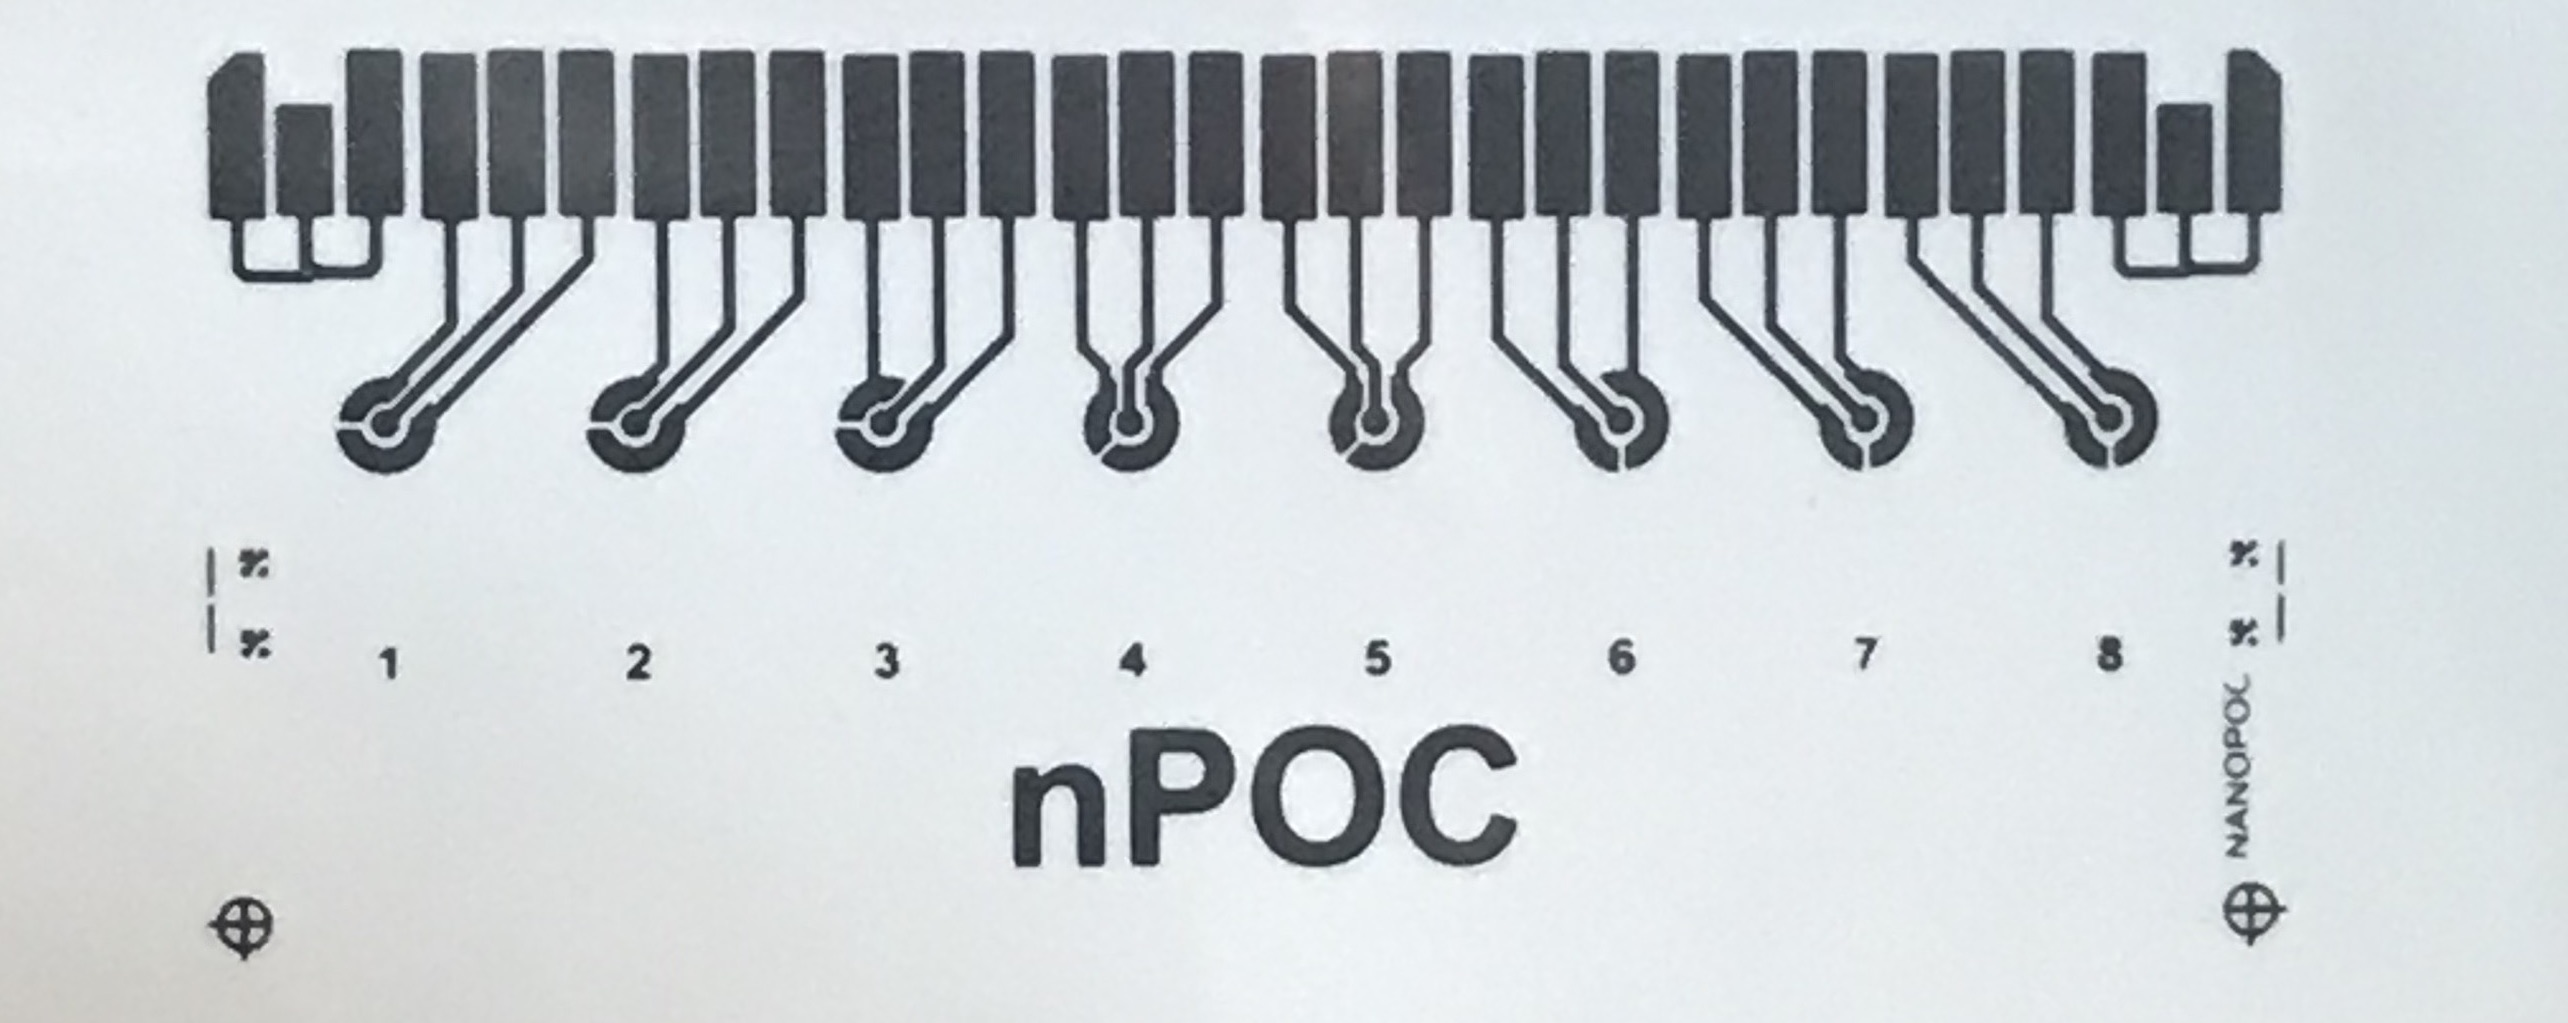
\includegraphics[width=0.5\textwidth]{Figures/Figura_Electrodos_nPOC}
  \caption{Electrochemical Cells}
  \label{fig:Figura_Electrodos_nPOC}
\end{figure}

\section{Preparation of image patterns}

\subsection{Preliminary measurements}
As a first instance, the different components of carbon printed electrochemical cells were measured. It was concluded that the working electrodes (from now on \emph{WE}) have a diameter of 1 mm, where the gold ink will be deposited. The separation between \emph{WE} and reference electrode (from now \emph{RE}) and counter electrode (from now \emph{CE}) is 400 $\mu$m. The distance between two \emph{WE} is 9 mm and each cartridge has eight sensors. This measured distance between two \emph{WE} corresponds to the separation of an eight-channel micro pipette, used in laboratories. (Figure ~\ref{fig:Figura_medicion_celdas})

\begin{figure}[H]
  \centering
    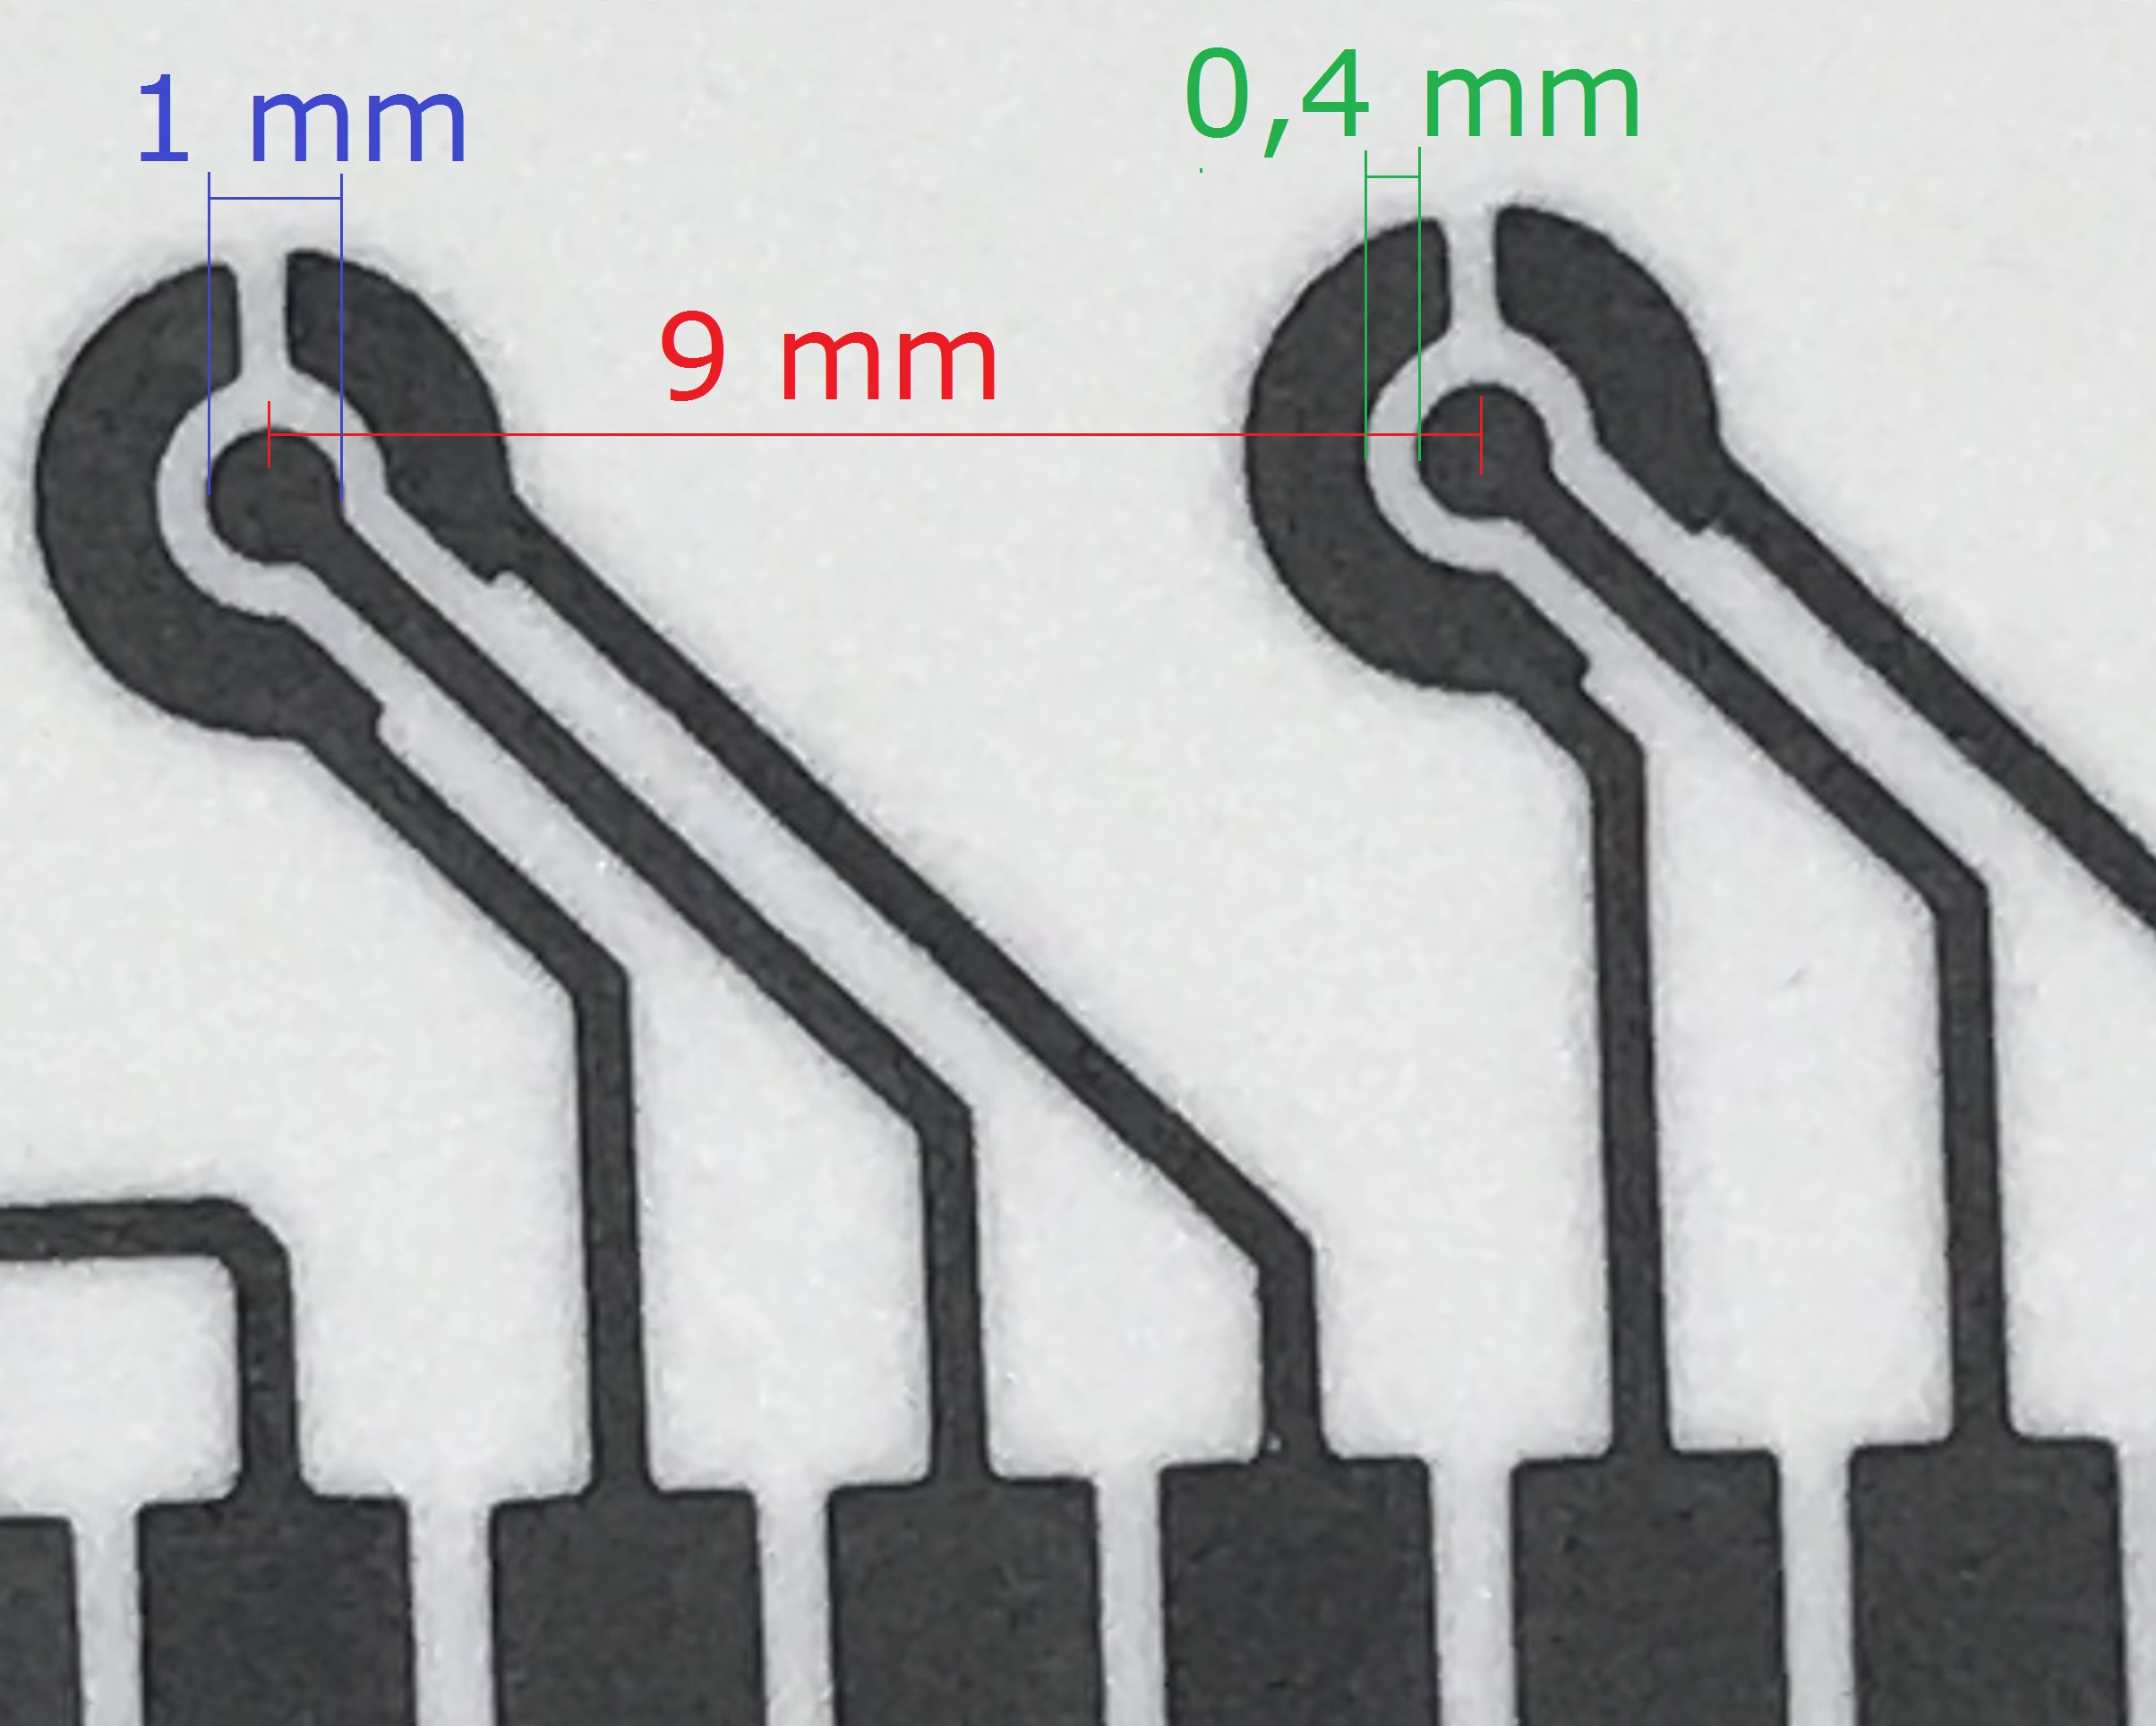
\includegraphics[width=0.5\textwidth]{Figures/Figura_medicion_celdas}
  \caption{Dimensional measurements on substrate.}
  \label{fig:Figura_medicion_celdas}
\end{figure}

Since the carbon prints were made by a company dedicated to industrial screen printing, the biosensors are manufactured in two columns and six rows giving a total of twelve sensors per substrate of A4 size (Figure ~\ref{fig:Figura_sensores_hoja_A4}). To have an accurate follow-up of the work to be carried out on each sample, they are listed taking advantage of their already printed carbon name as \textit{nPoc} from 1 to 5. (Figure ~\ref{fig:Figura_ejemplo_numeracion_nPoc})

\begin{figure}[H]
  \centering
    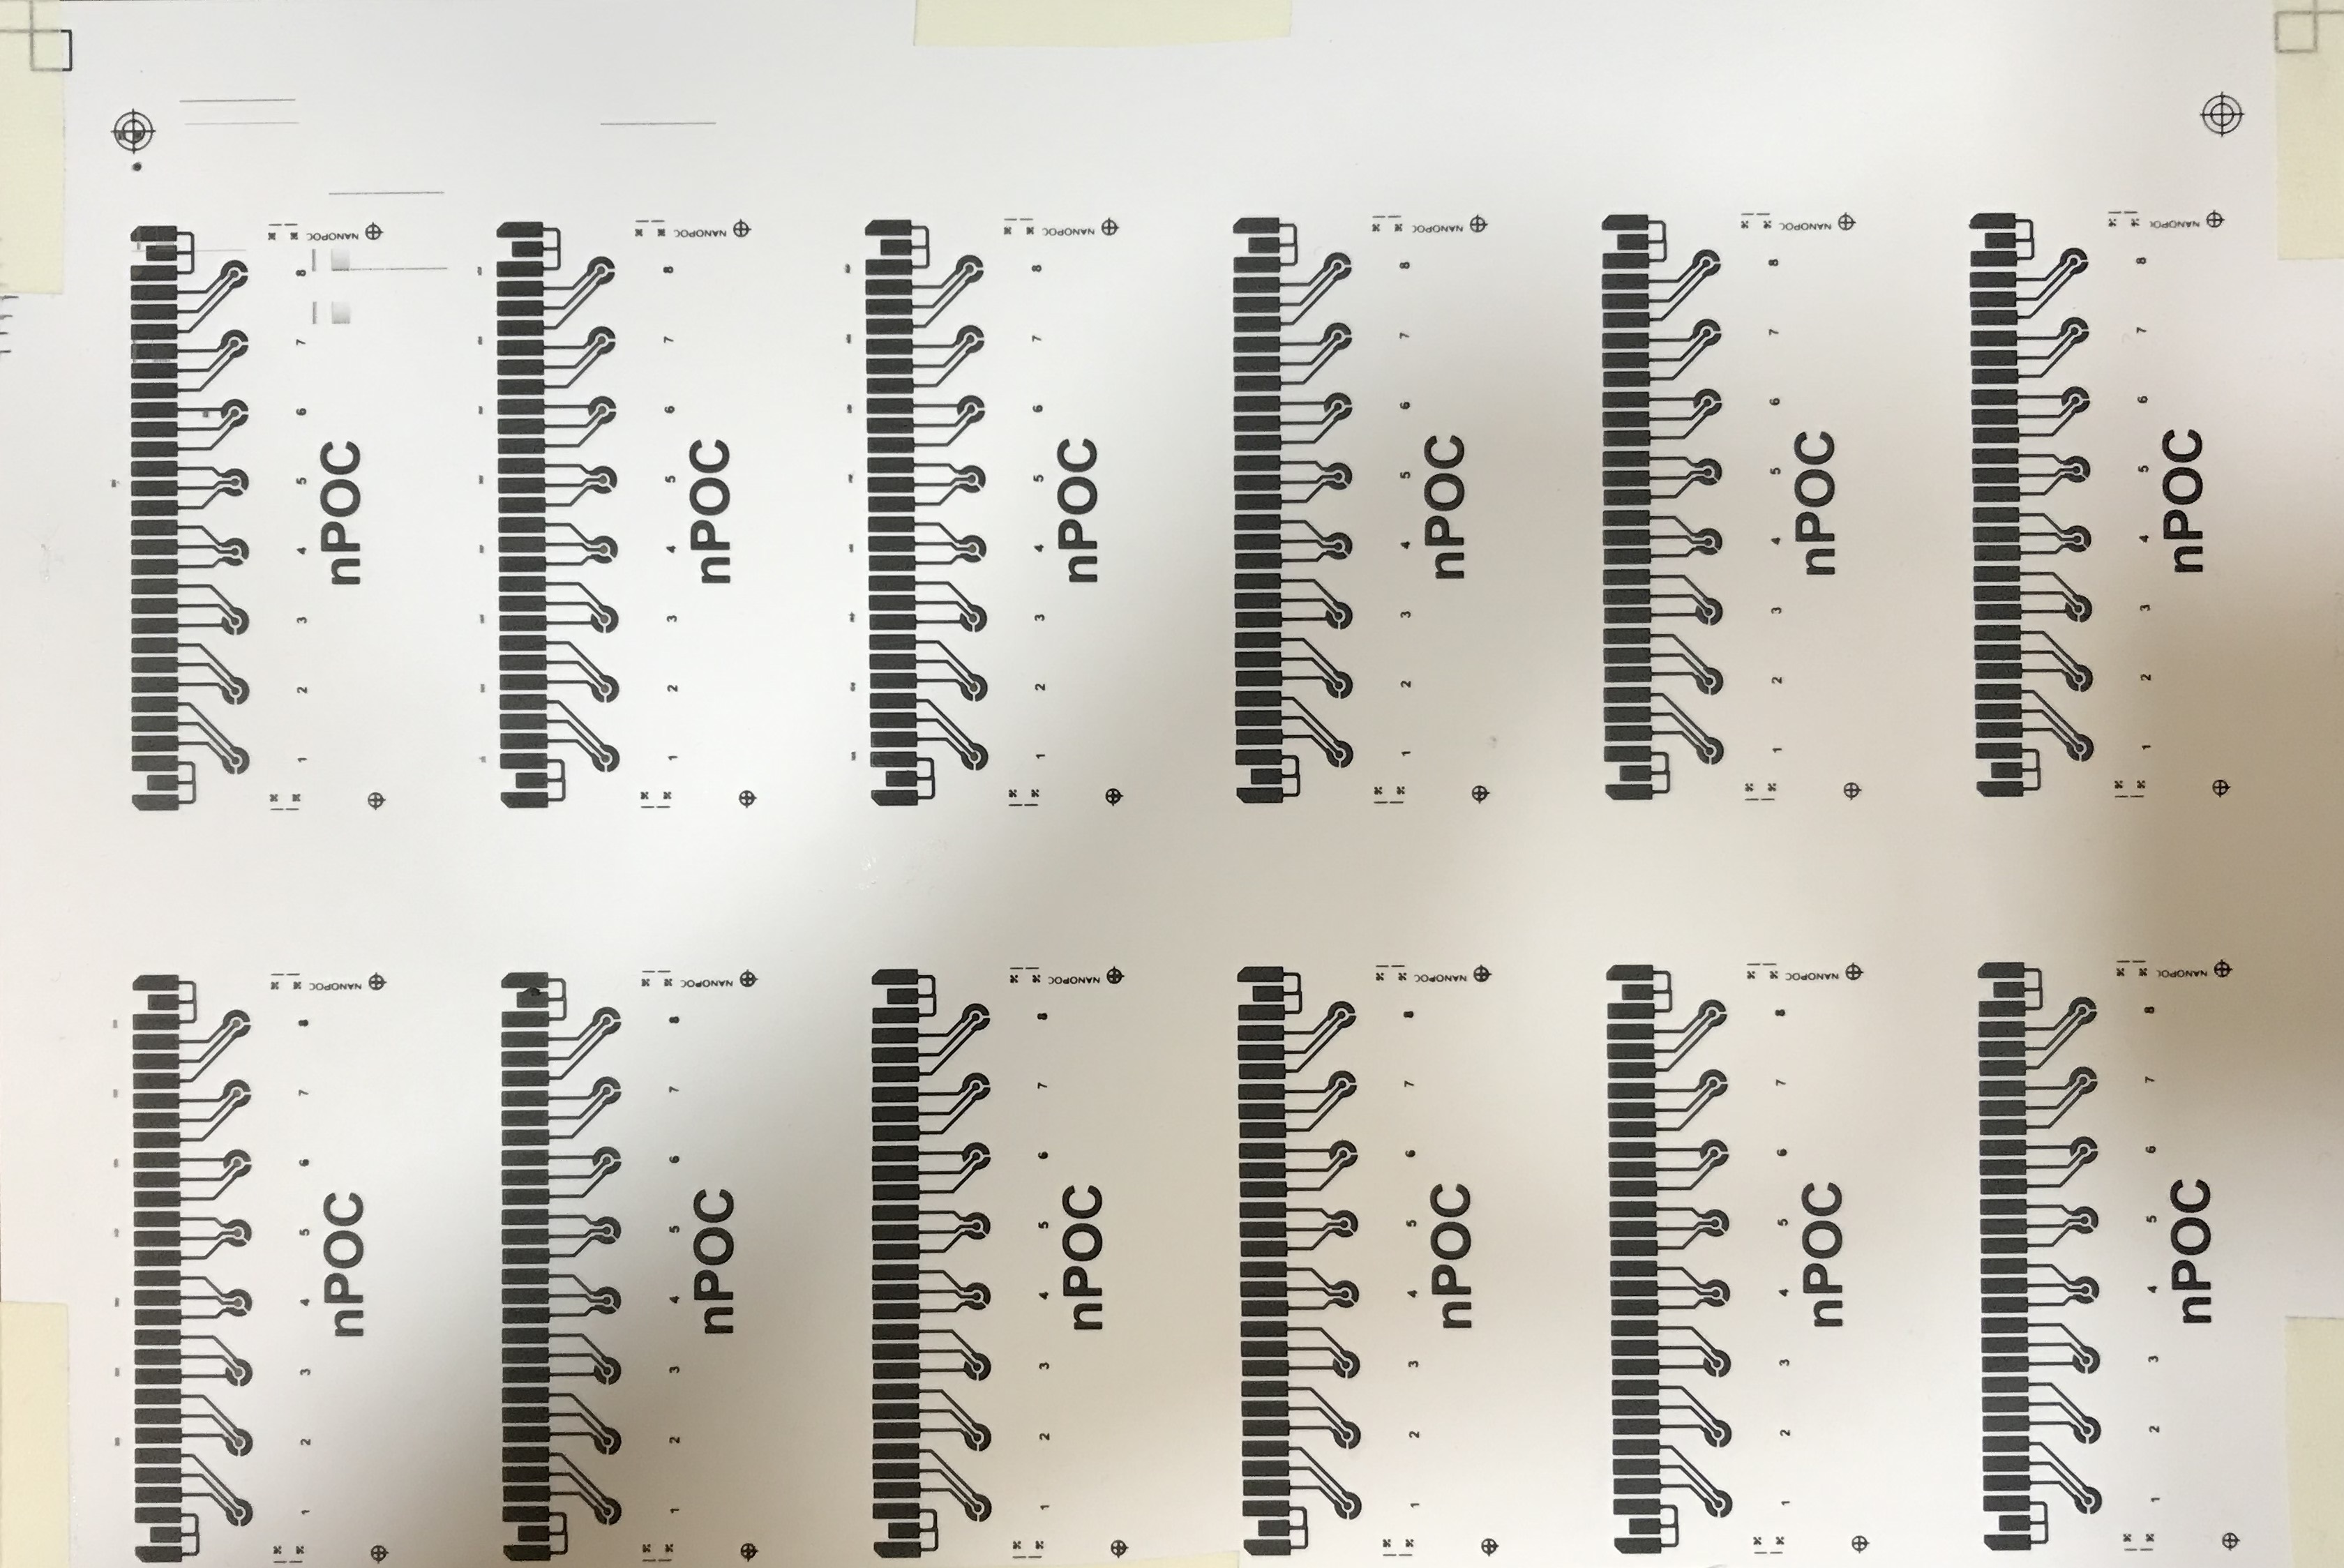
\includegraphics[width=0.5\textwidth]{Figures/Figura_sensores_hoja_A4}
  \caption{Screen printing of biosensors on A4 sheet.}
  \label{fig:Figura_sensores_hoja_A4}
\end{figure}

\begin{figure}[H]
  \centering
    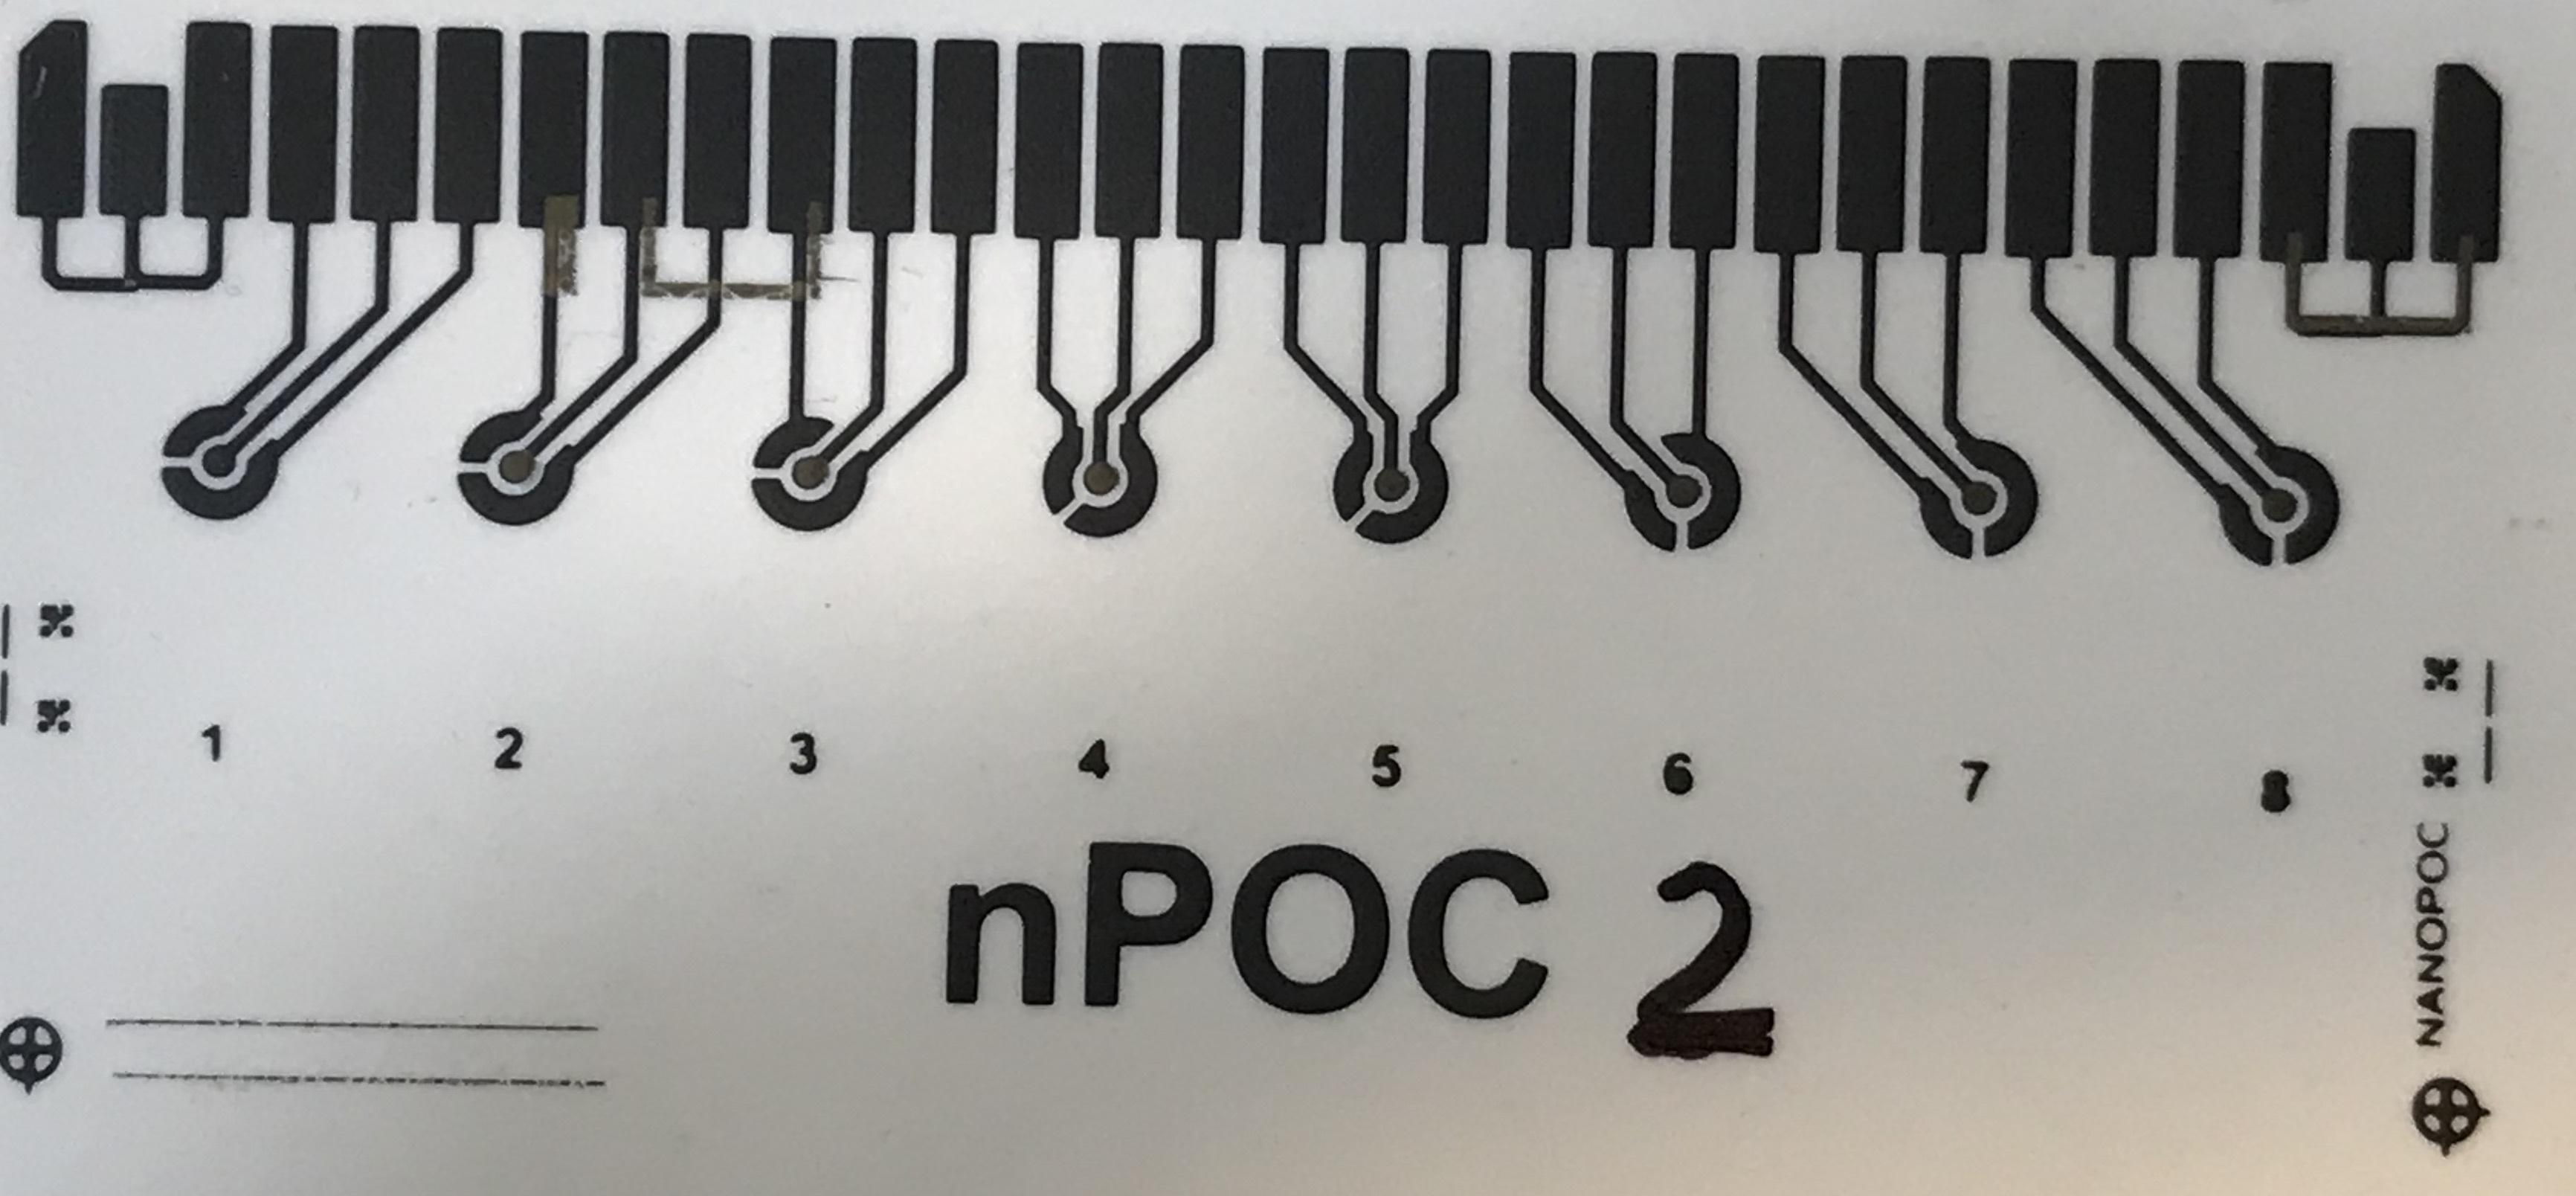
\includegraphics[width=0.5\textwidth]{Figures/Figura_ejemplo_numeracion_nPoc}
  \caption{nPoc2 sensor numbering example.}
  \label{fig:Figura_ejemplo_numeracion_nPoc}
\end{figure}

\subsection{Print pattern designs}
\label{subsec:diseno_impresion}
Once the necessary measurements have been obtained from the sensors, the printing patterns are designed. The professional free and open source InkScape graphic vector editor was used for this \cite{Inkscape} (Figure ~\ref{fig:Figura_Inkscape}).

\begin{figure}[H]
  \centering
    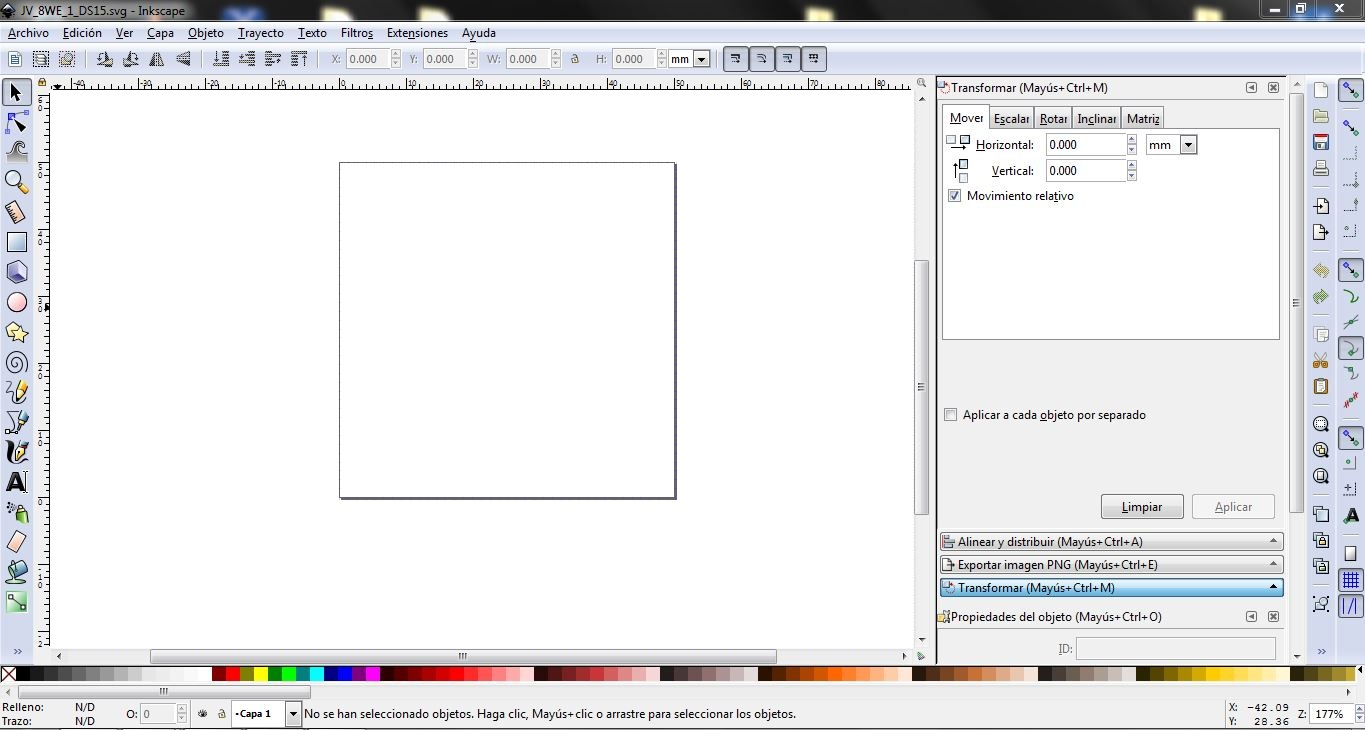
\includegraphics[width=0.65\textwidth]{Figures/Figura_Inkscape}
  \caption{Free and open source professional graphic vector editor.}
  \label{fig:Figura_Inkscape}
\end{figure}

Four drawings were made with two possible resolutions. The first drawings correspond to a circle of 1 mm and 1.1 mm in diameter, the size of one \emph{WE} and 100 $\mu$m more in the second. This is to establish whether using the same diameter achieves optimum coverage with the gold nanoparticle ink or if an offset needs to be added. The other two drawings consist of an array of eight 1 mm diameter circles spaced 9 mm apart and an array of eight 1.1 mm diameter circles with the same spacing (Figure ~\ref{fig:Figura_Diseno_Circulos}). The resolutions used were 1693.33 and 1270 dpi, later the reason for said resolutions will be explained.

\begin{figure}[H]
  \centering
    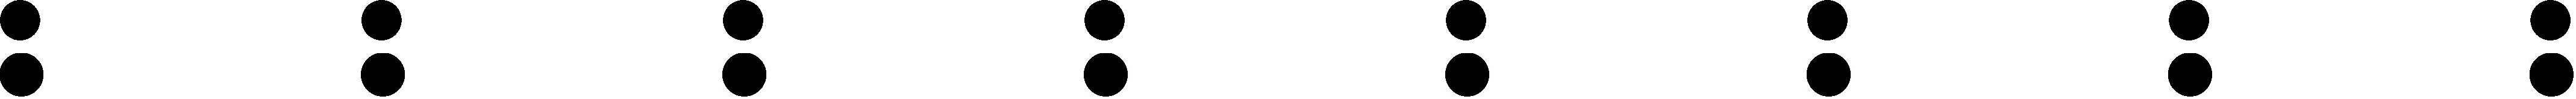
\includegraphics[width=0.5\textwidth]{Figures/Figura_Diseno_Circulos}
  \caption{1 and 1.1 mm print designs.}
  \label{fig:Figura_Diseno_Circulos}
\end{figure}

Since the printer software (\textit{Dimatix Drop Manager}) does not detect color or grayscale images, they must be converted to monochrome 1-bit files. This way, the only thing present in the image are black or white pixels, corresponding to where a drop of ink should be ejected or not. The format that can save 1-bit images is the Windows bitmap (or BMP for its acronym in English), and therefore it is the only external format supported by the \textit{Dimatix Drop Manager}. Conversion to BMP format is done using \textit{Microsoft Paint} Software. By zooming in on the same image in PNG and BMP format, the differences can be seen with the naked eye (Figure ~\ref{fig:Figura_comparacion_png_bmp}).

\begin{figure}[H]
  \centering
    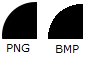
\includegraphics[width=0.5\textwidth]{Figures/Figura_comparacion_png_bmp}
  \caption{Comparison of PNG and BMP files.}
  \label{fig:Figura_comparacion_png_bmp}
\end{figure}

Once the files are obtained in the correct format, the printer parameters can be prepared and set up.

\section{Printer setup and calibration}
\label{sec:calib_impresora}
After preparing, placing and configuring the ink cartridge and the substrate (see \hyperref[chap:apendiceA]{Annex A}), the design or pattern to be printed must be added.

For this the DMP software offers two options. The first allows drawing with the same program, adding positions (X and Y coordinates) and the desired thickness; the second allows you to import images in monochrome BMP format. The creation of designs using the DMP software only allows basic shapes and, above all, shaped by straight lines. For more complex drawings, the external design procedure explained in the section on print pattern design is recommended (Chapter 3, \hyperref[subsec:diseno_impresion]{section 3.1.2}).

For any of the two options, reference coordinates can be added, used to locate the print on the substrate and a $``$\textit{Leader Bar}$``$ with the possibility of setting its width and its distance (\textit{Gap}) with the design to be printed. This last function is a commonly used procedure to keep the nozzles active and a uniform flight speed of the drops at the start of printing, improving the quality of the pattern. It must be taken into account that the $``$\textit{Leader Bars}$``$ must be located inside the substrate, otherwise ink will be being ejected onto the printer plate (Figure ~\ref{fig:Figura_Leader_Bar}).

\begin{figure}[H]
  \centering
    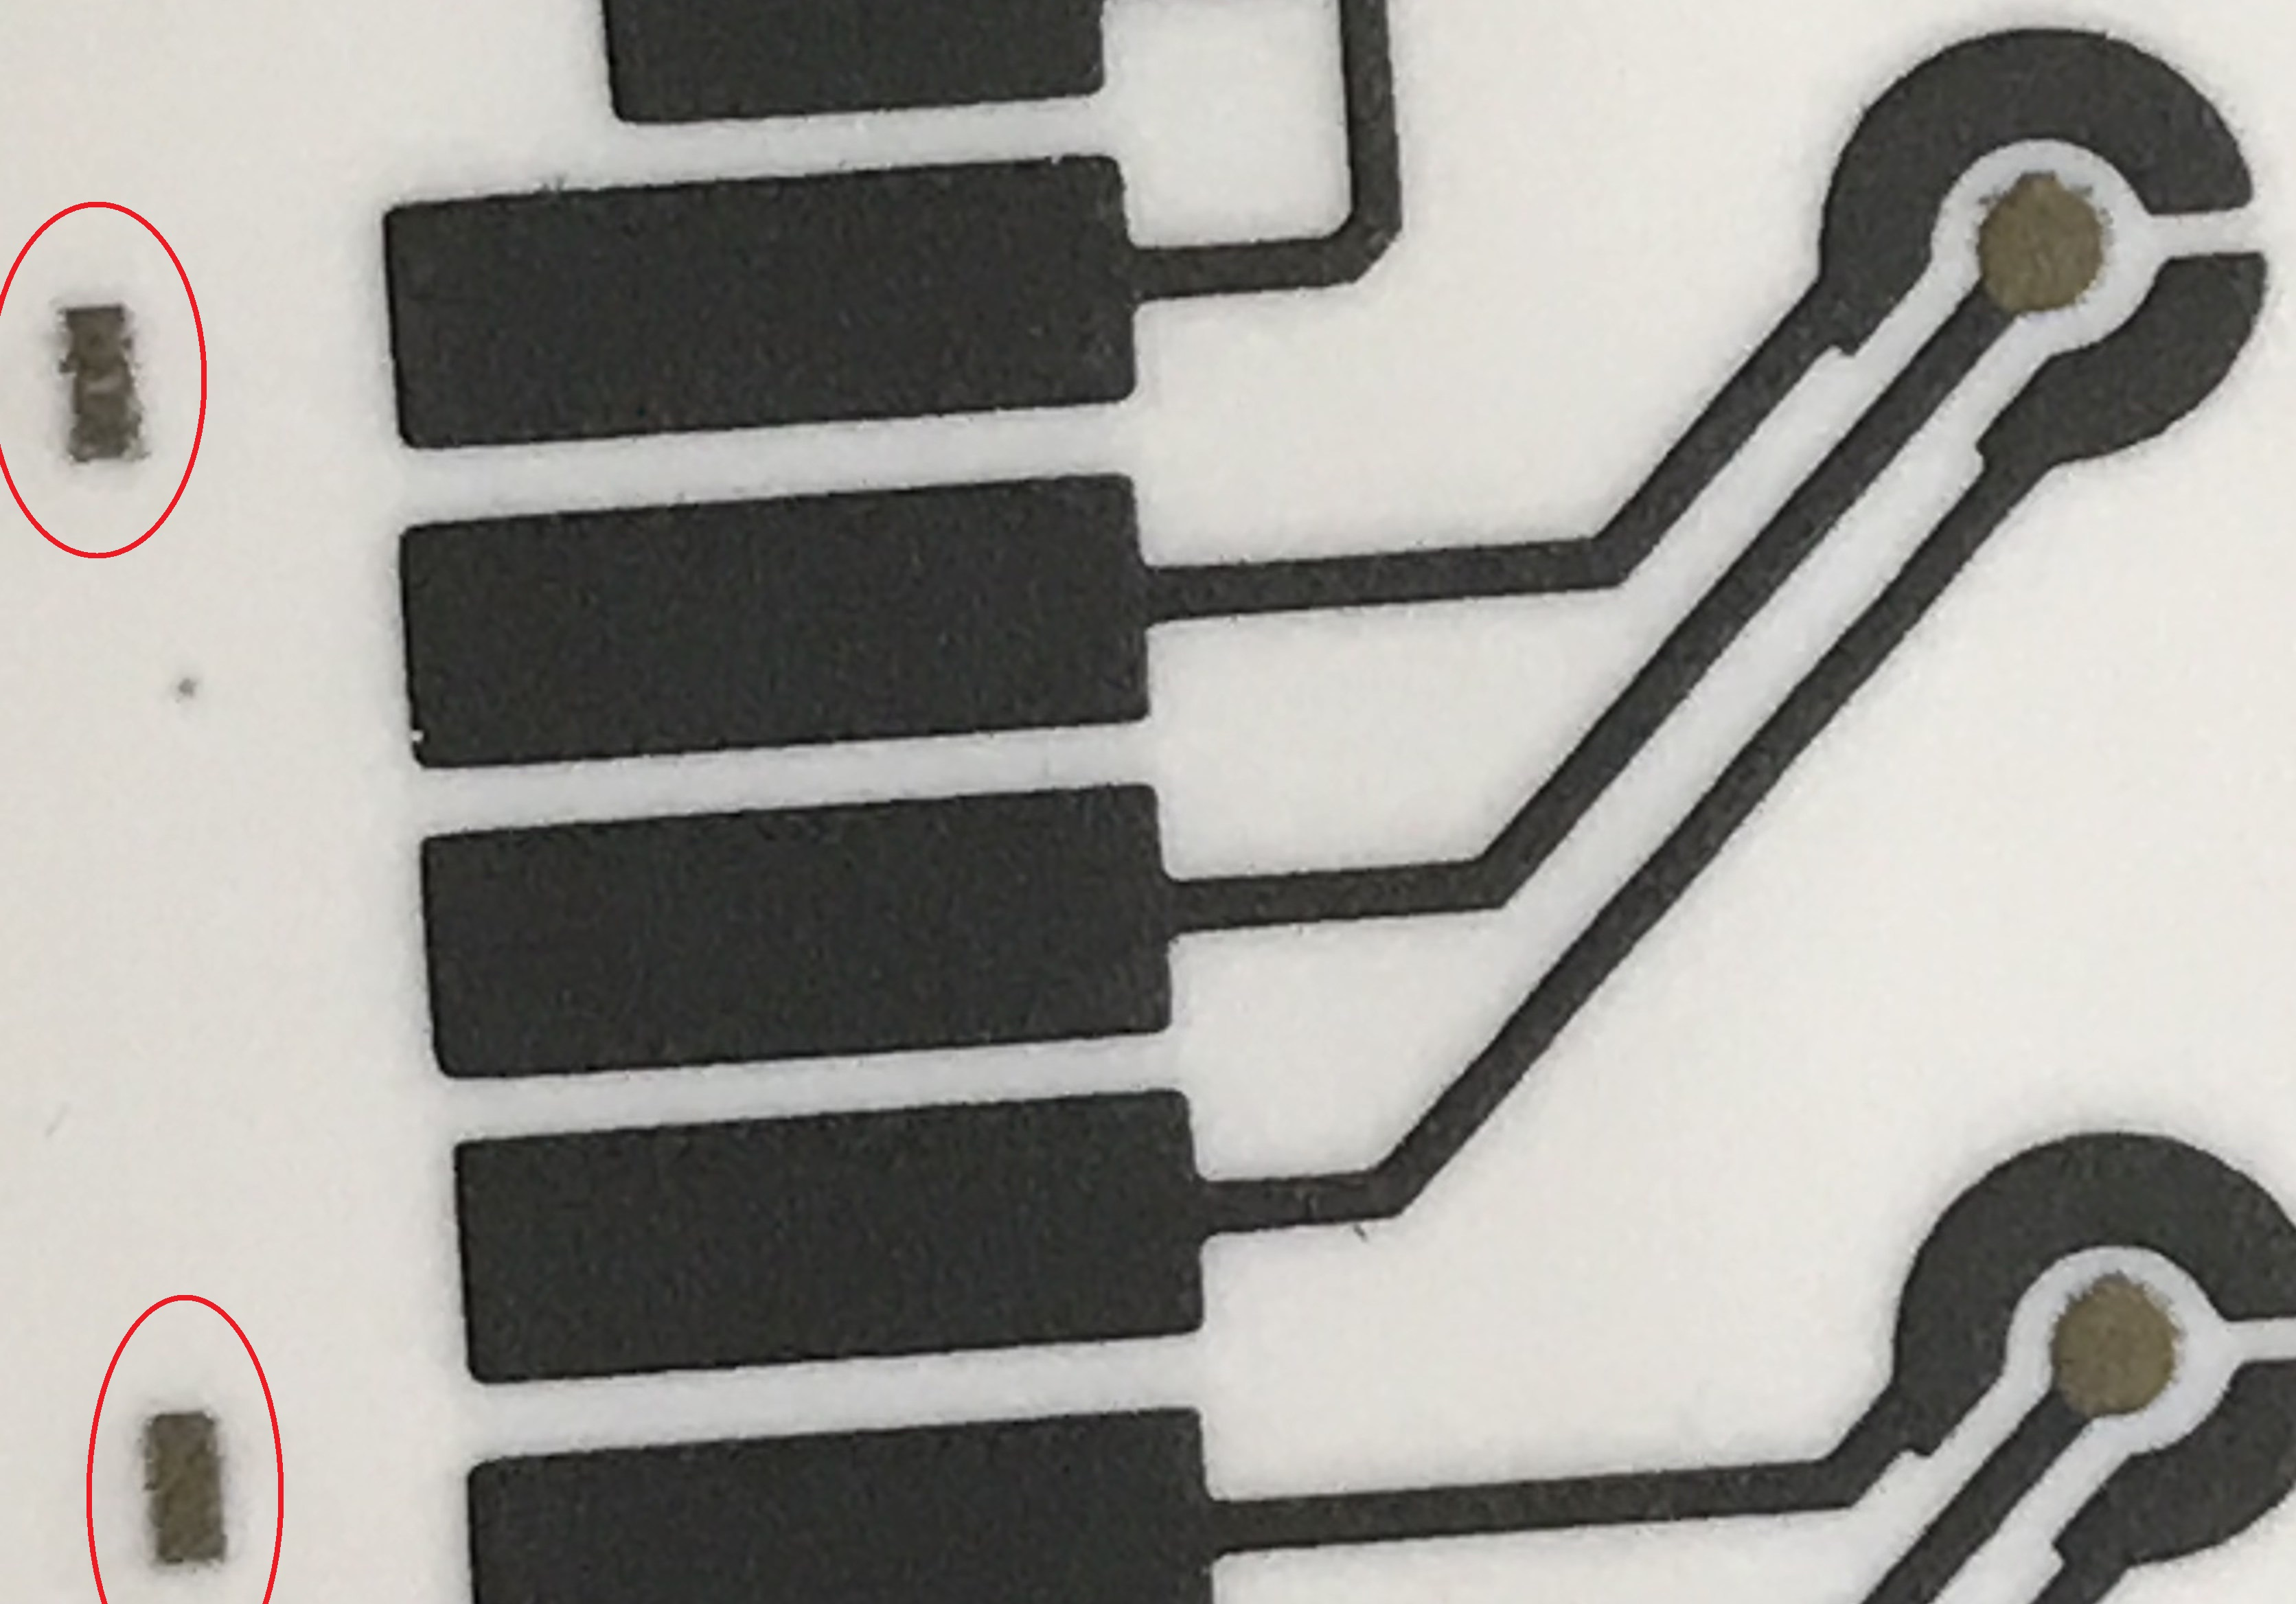
\includegraphics[width=0.5\textwidth]{Figures/Figura_Leader_Bar}
  \caption{$``$\textit{Leader Bars}$"$ printed on substrate.}
  \label{fig:Figura_Leader_Bar}
\end{figure}

At this point, if it was not done previously, it is advisable to calibrate the ejection voltages of the Nozzles that will be used by means of the $``$\textit{Drop Watcher}$"$ (Figure ~\ref{fig:Figura_nozzles}). This system consists of a camera oriented at 45º from the horizontal plane with focus on the Nozzles of the head that, by means of a strobe light, allows to photograph or film the operation of the holes in the head (Drop ejection).

\begin{figure}[H]
  \centering
    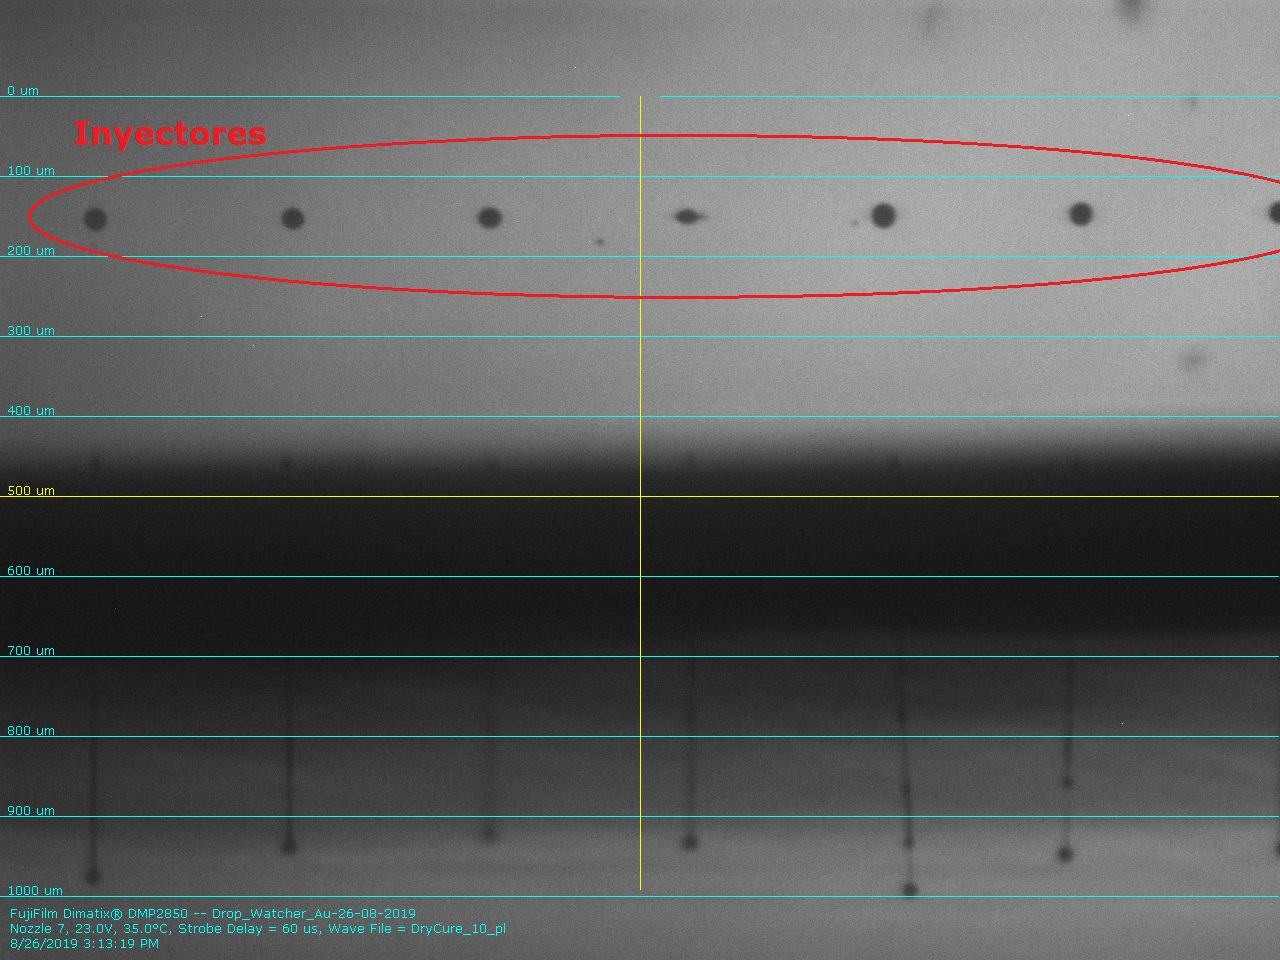
\includegraphics[width=0.5\textwidth]{Figures/Figura_nozzles}
  \caption{Nozzles seen from the $``$\textit{Drop Watcher}$"$ camera.}
  \label{fig:Figura_nozzles}
\end{figure}

Then, using the fiducial camera, the drops and substrate alignment processes are carried out and the coordinates where the printing begins are set.

Alignment of the substrate is accomplished by \textit{Theta} calibration. For this procedure, two points must be selected that are aligned on the substrate. In this case, the carbon print includes different alignment points. The smallest ones will be used to obtain greater precision, and thus minimizing the error due to the minimum width of the screen printing manufacturing (Figure ~\ref{fig:Figura_alineacion_theta}).

\begin{figure}[H]
  \centering
    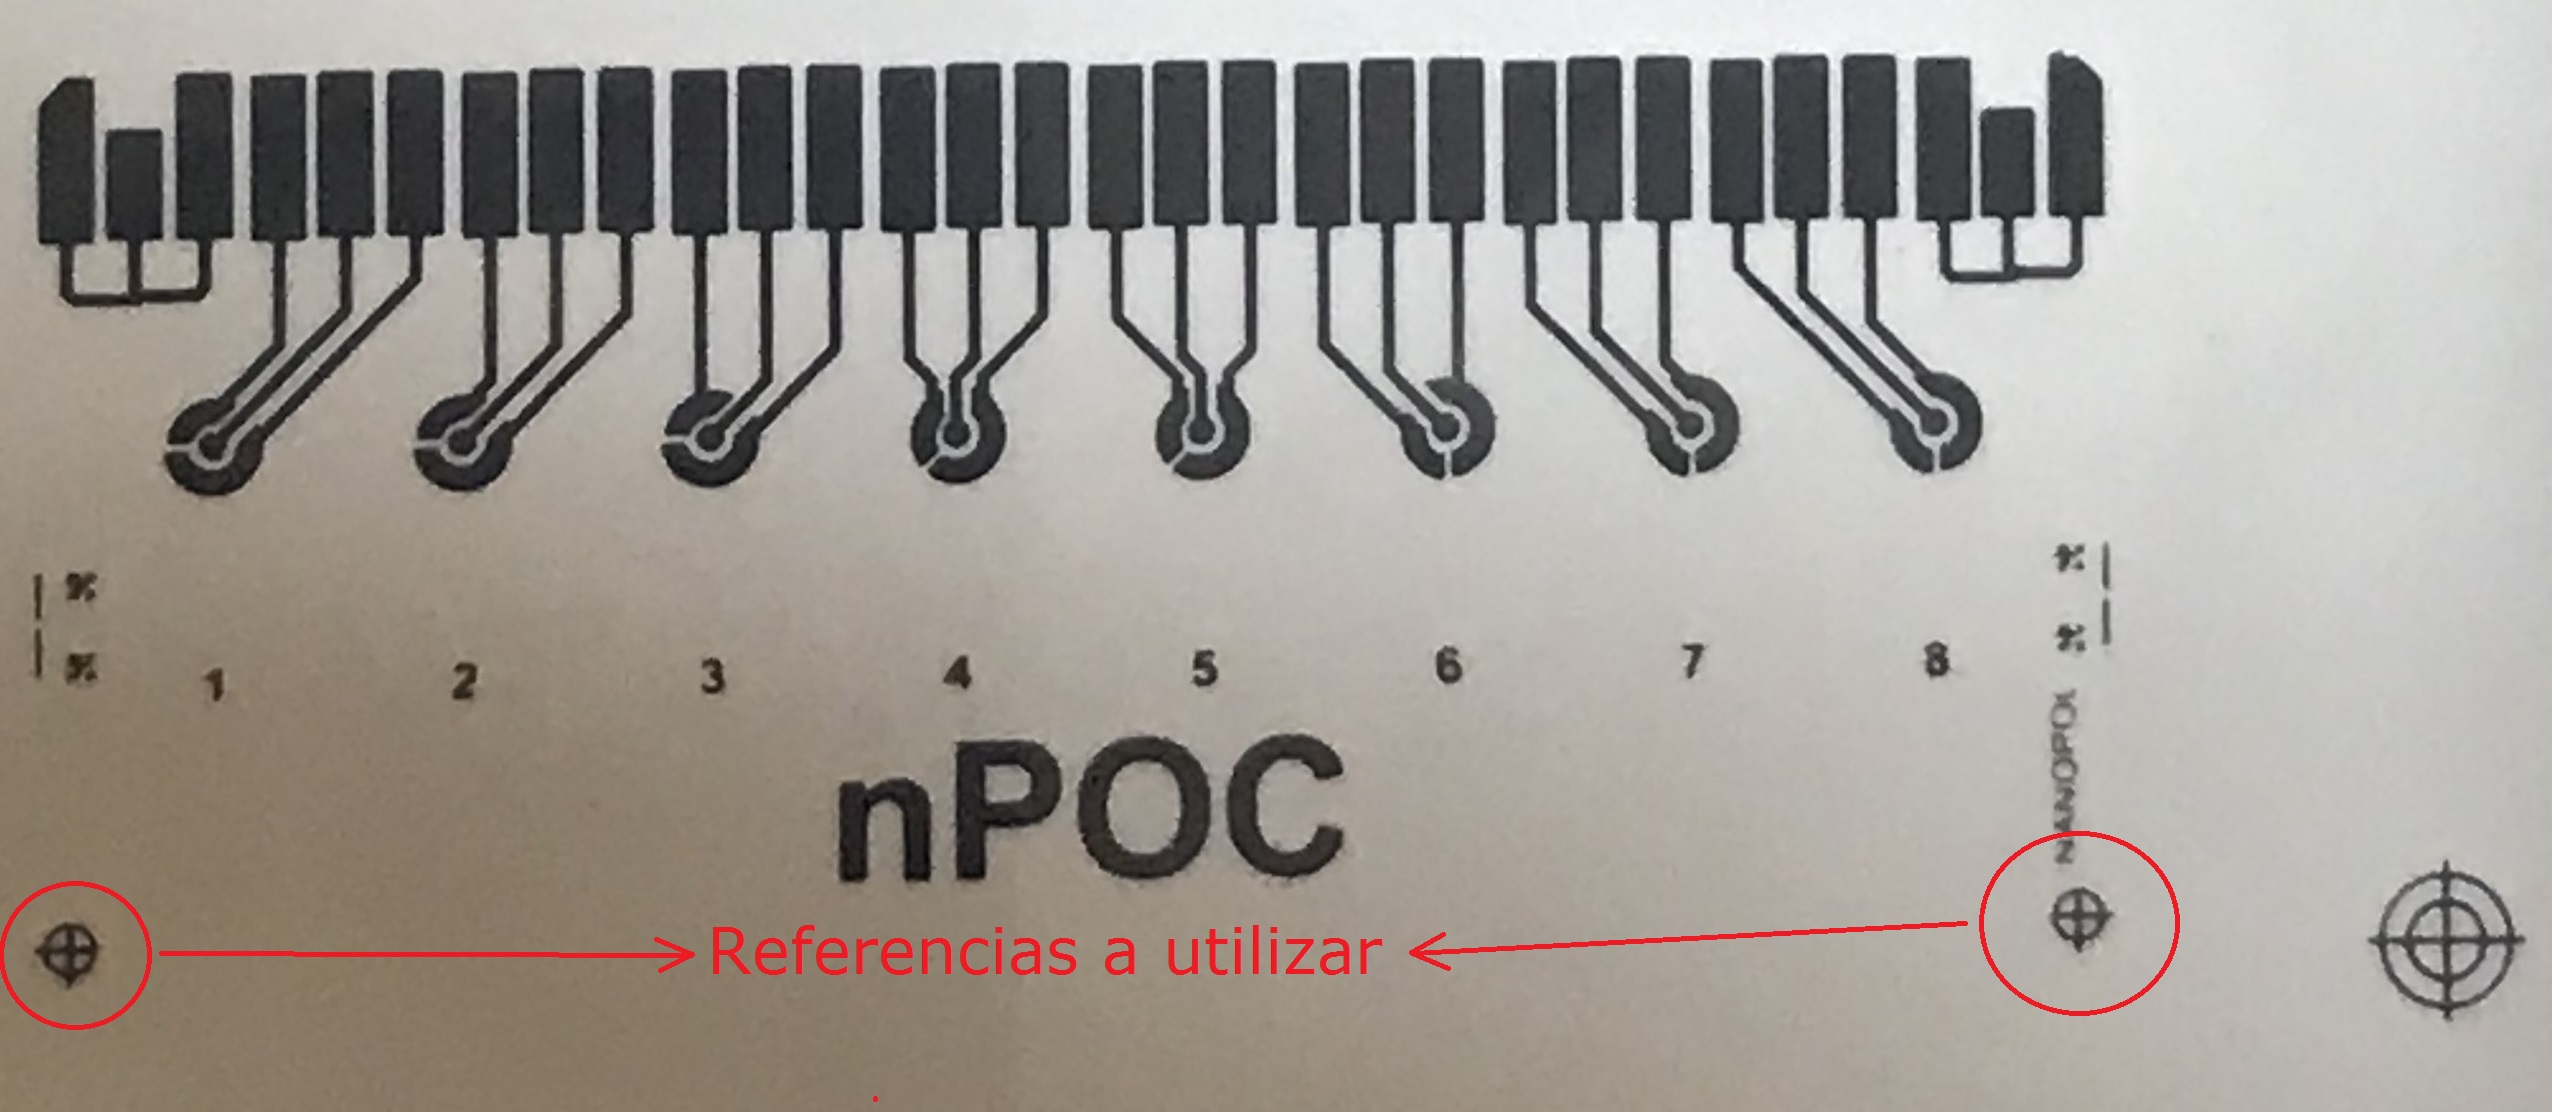
\includegraphics[width=0.5\textwidth]{Figures/Figura_alineacion_theta}
  \caption{References used for the \textit{Theta} calibration.}
  \label{fig:Figura_alineacion_theta}
\end{figure}

Although the alignment objects appear to be fine and regular to the naked eye, when using the fiducial camera it is observed that it is not easy to determine the midpoint (Figure ~\ref{fig:Figura_alineacion_theta2}).

\begin{figure}[H]
  \centering
    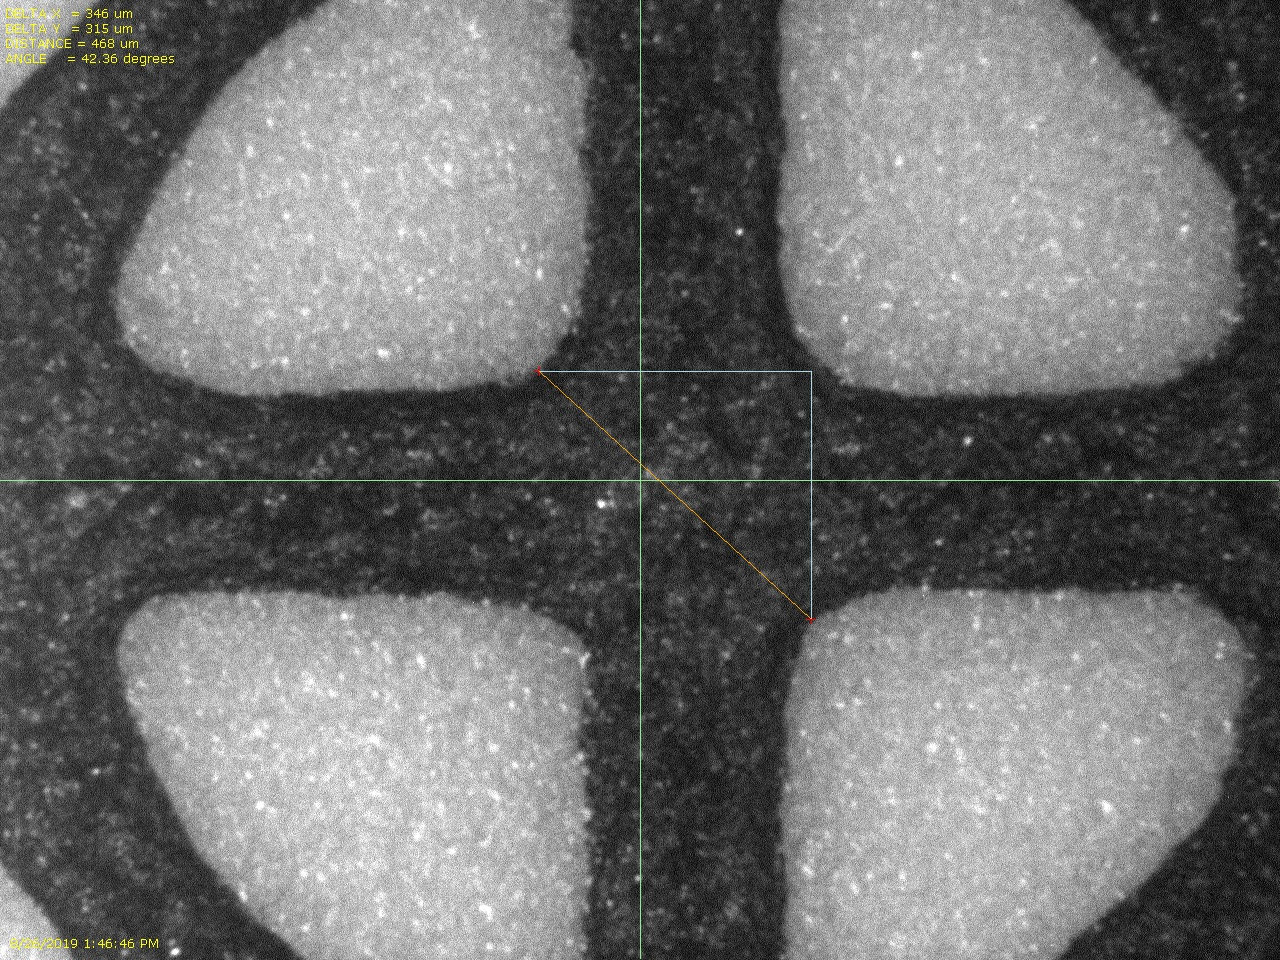
\includegraphics[width=0.4\textwidth]{Figures/Figura_alineacion_theta2}
  \caption{Alignment object seen with fiducial camera.}
  \label{fig:Figura_alineacion_theta2}
\end{figure}

Following the alignment of the substrate, it must be defined the spacing between drops that will be used when printing. This parameter is identified as $``$\textit{Drop Spacing}$"$ (from now on \emph{DS}) and, to determine it, a drop pattern with the different spacings allowed by the printer, called $``$\textit{Line Pattern}$"$, was used (Figure ~\ref{fig:Figura_Line_Pattern_Micro50X}). After printing, it is decided wich \emph{DS} generates the best defined line, both in continuity and in homogeneity of width and thickness, on the substrate to be used. For the gold ink on \textit{Valox} it was decided to use a spacing of 15 $\mu$m between drops, since it shows a continuous line without generating ink $``$\textit{Clusters}$"$.

\begin{figure}[H]
  \centering
    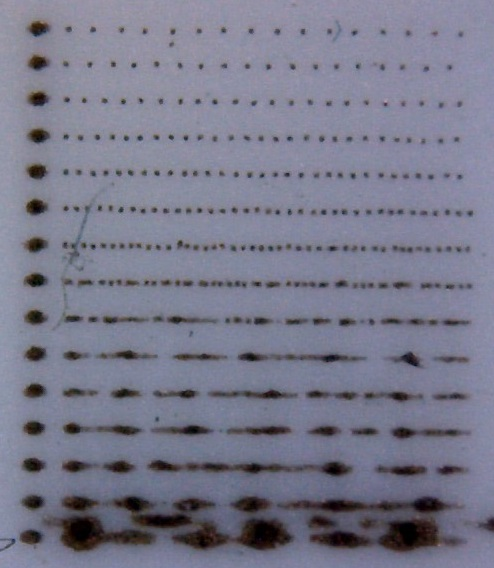
\includegraphics[width=0.35\textwidth]{Figures/Figura_Line_Pattern_Micro50X}
  \caption{$``$\textit{Line Pattern}$"$ viewed under a 50X microscope.}
  \label{fig:Figura_Line_Pattern_Micro50X}
\end{figure}

Once the \emph{DS} is defined, the resolution of the design to be printed is adjusted. In the case of 15 $\mu$m $``$\textit{Drop Spacing}$"$ between drops, a resolution of 1693.33 dots per inch (from now on \emph{dpi}) is used. The printer's instruction manual \cite{DimatixUM} provides a table with the resolution that the design should have and the angle at which the cartridge should be configured for each \emph{DS} (Figure ~\ref{fig:Figura_Tabla_angulos}).

\begin{figure}[H]
  \centering
    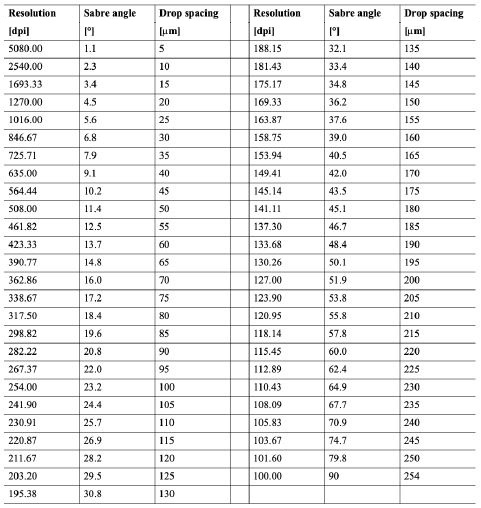
\includegraphics[width=0.5\textwidth]{Figures/Figura_Tabla_angulos}
  \caption{Table of resolutions and angles for each \emph{DS}.}
  \label{fig:Figura_Tabla_angulos}
\end{figure}

Next the $``$\textit{Drop Offset}$"$ calibration must be performed. This procedure compensates the error between the point where the fiducial camera is $``$looking$"$ and the position where the cartridge is printing. That is, it compensates the flight of the ink drops between its ejection from the head until it hits the substrate. For this, the printer makes a continuous line of 10 mm on the X axis followed by a point at 1 mm from the line. Calibration is performed once this point is located with the fiducial camera and $``$\textit{clicked}$"$ on it, as centered as possible (Figure ~\ref{fig:Figura_prueba_Drop_Spacing}).

\begin{figure}[H]
  \centering
    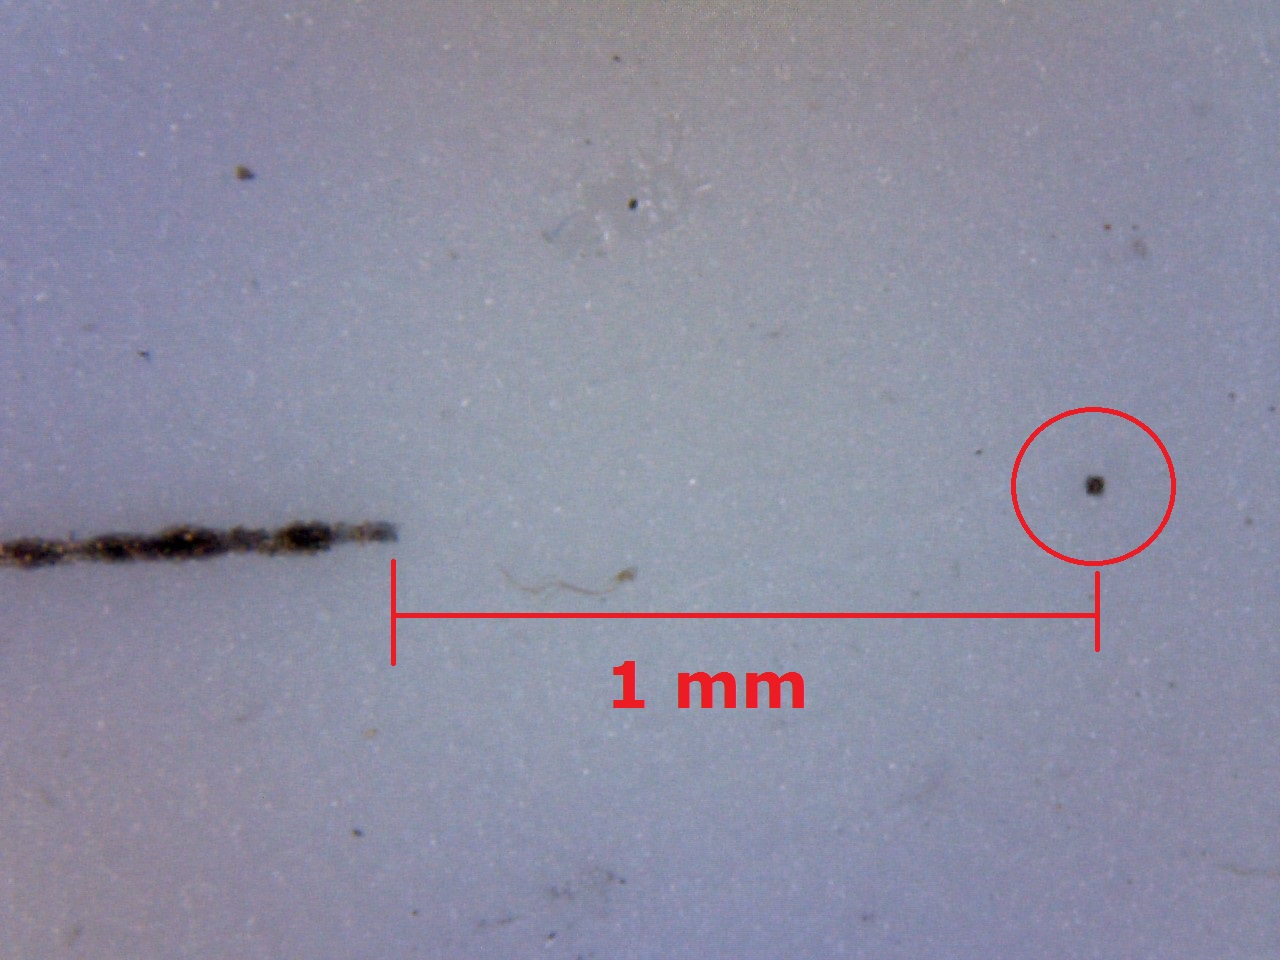
\includegraphics[width=0.5\textwidth]{Figures/Figura_prueba_Drop_Spacing}
  \caption{End of line and point of $``$\textit{Drop Offset}$"$ procedure, seen with a 1000X microscope.}
  \label{fig:Figura_prueba_Drop_Spacing}
\end{figure}

The fiducial camera is an element of the reel where the cartridge is placed (Figure ~\ref{fig:Figura_Camara_Fiducial}). This is used for the alignment procedures of the substrate, the calibration of the flight time of the ejected drops, the checkup of the substrate and the impressions on it or measurements on the surface placed on the stage. It has a field of view of 1.62 mm wide and 1.22 mm high, with a resolution of 2.54 $\mu$m per pixel.

\begin{figure}[H]
  \centering
    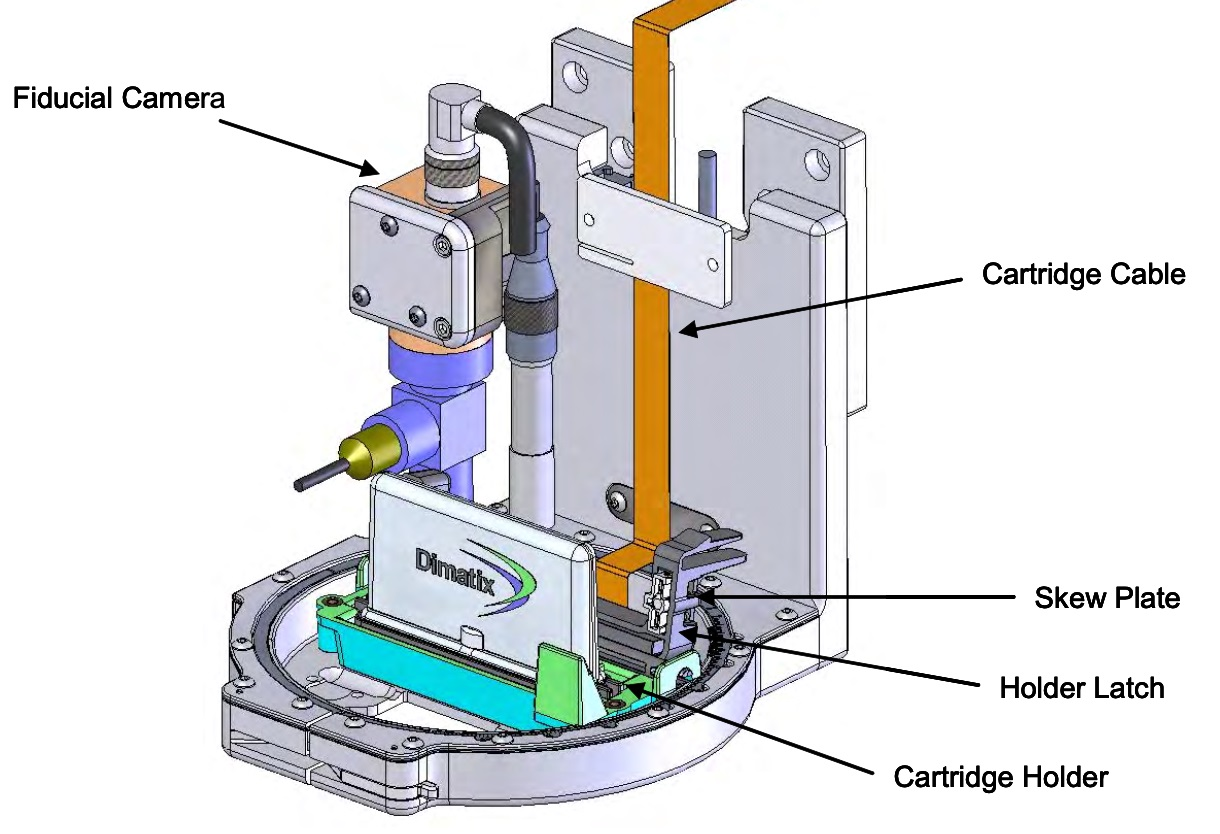
\includegraphics[width=0.5\textwidth]{Figures/Figura_Camara_Fiducial}
  \caption{Illustration of the different components of the printer reel.}
  \label{fig:Figura_Camara_Fiducial}
\end{figure}

As the last configuration before start printing, the coordinates of the substrate where it will start ($``$\textit{Print Origin}$"$) or a reference must be defined, which will agree with those defined in the design ($``$\textit{Reference Point}$"$).

If it is decided to use the point where it will start printing, \textit{Set Print Origin} function of the fiducial chamber must be chosen. On the other hand, if it will use a reference point of the design with the substrate, \textit{Set Reference Point} function must be configured (Figure ~\ref{fig:Figura_Ventana_Camara_Fiducial}). When using this last function, it must be taken into account that the reference point must be defined in the design before loading it in the image to print tab of the \textit{DMP} software.

\begin{figure}[H]
  \centering
    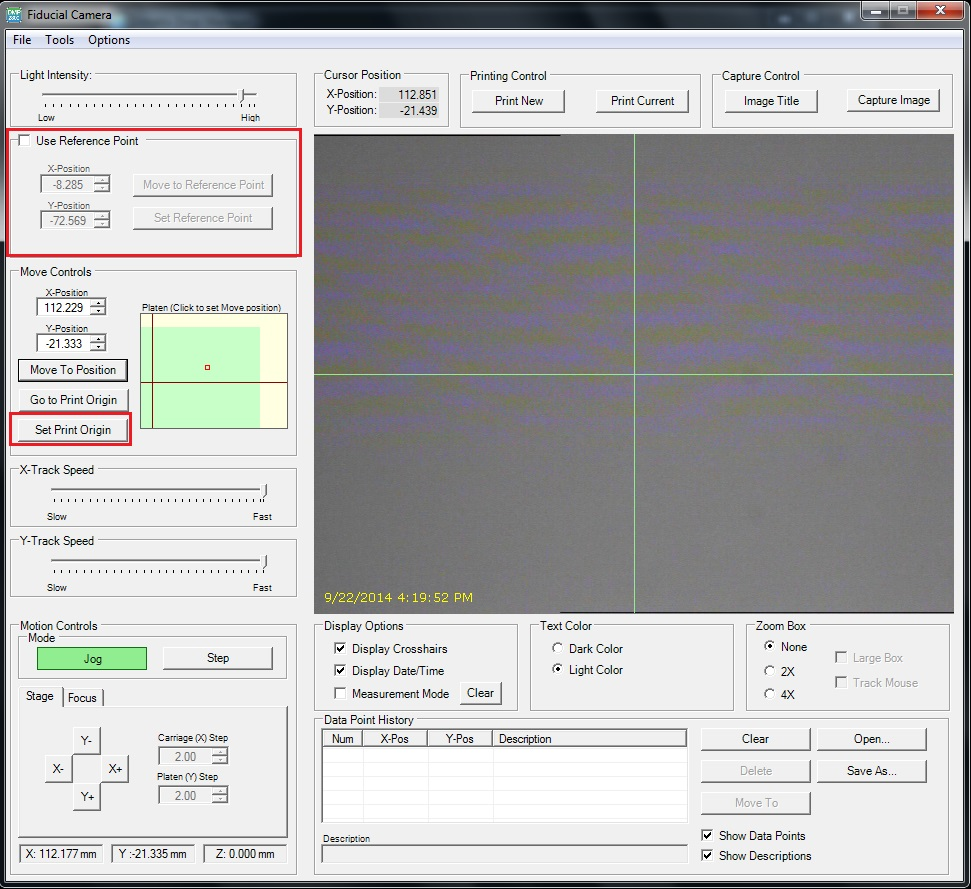
\includegraphics[width=0.5\textwidth]{Figures/Figura_Ventana_Camara_Fiducial}
  \caption{Fiducial camera window with options for \textit{Print Origin} and \textit{Reference Point}.}
  \label{fig:Figura_Ventana_Camara_Fiducial}
\end{figure}

For this work it was decided to use the center of the first circle as a reference point, aligning it with the working electrode 1 of the sensor. In this way, the other 7 circles were aligned with their respective electrode.

\section{Prints}
As a first test, a 1 mm diameter circle was printed on the carbon ink and on the \textit{Valox} substrate, to verify the behavior of the gold ink on both surfaces (Figure ~\ref{fig:Figura_Prueba_Sobre_Sustratos}).

\begin{figure}[H]
  \centering
    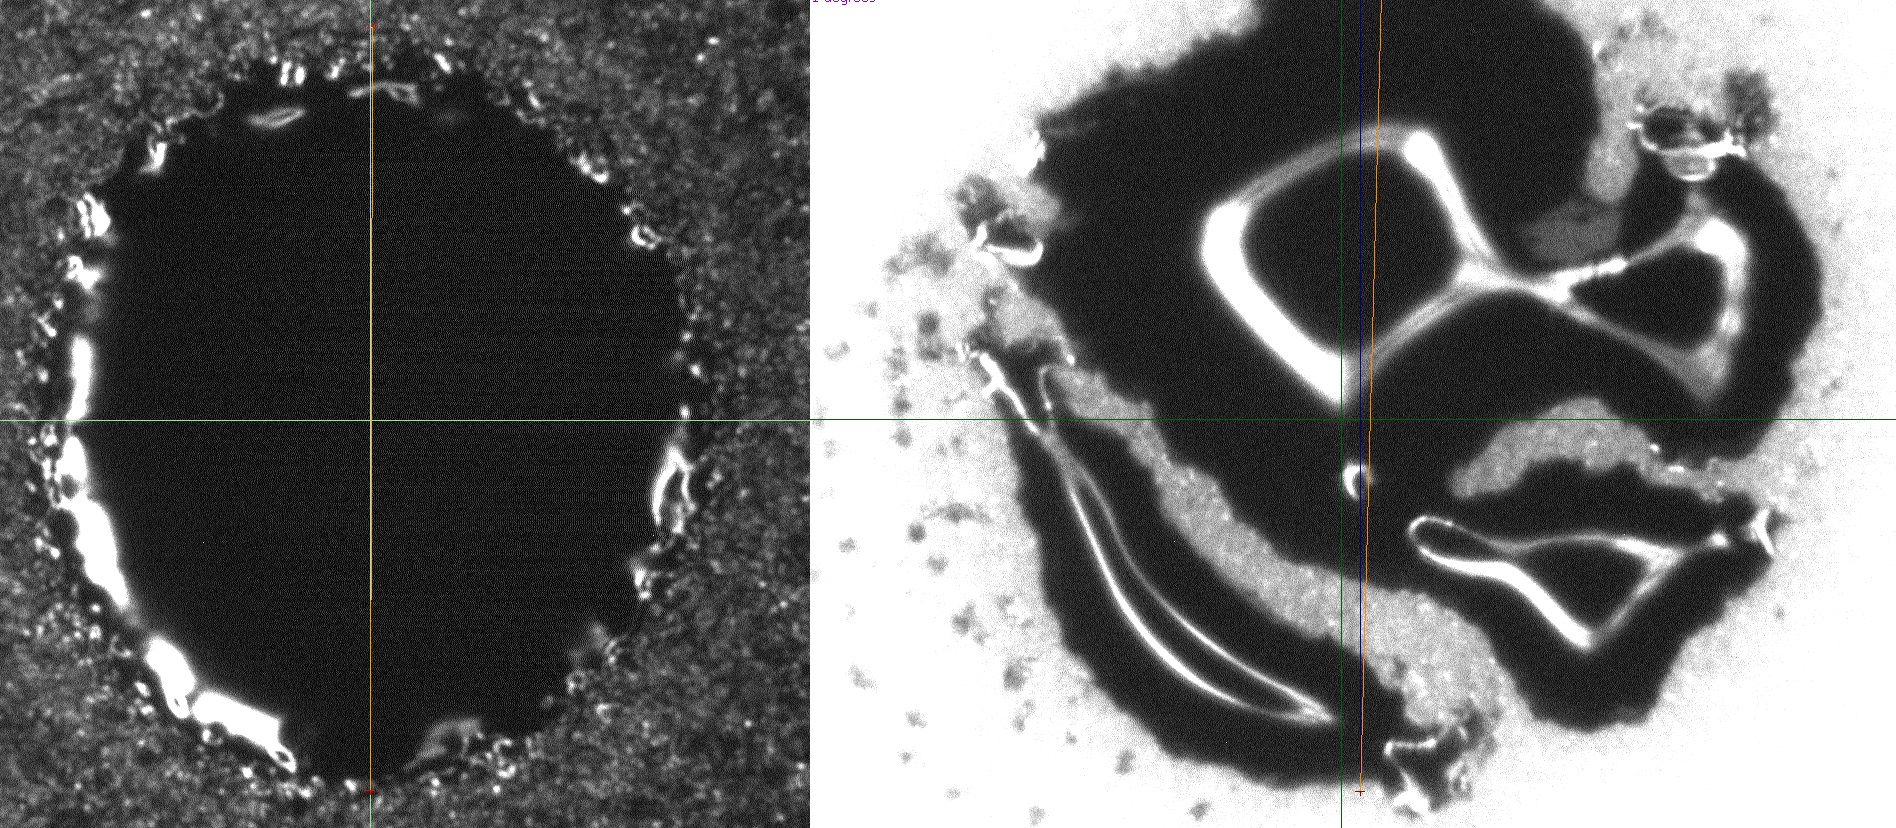
\includegraphics[width=0.5\textwidth]{Figures/Figura_Prueba_Sobre_Sustratos}
  \caption{Test of gold ink on carbon ink and \textit{Valox} substrate.}
  \label{fig:Figura_Prueba_Sobre_Sustratos}
\end{figure}

As expected, the gold ink shows better anchor on carbon than on the substrate.

The next test was to align the reference point with the drawing to be printed in the center of the first working electrode (WE1) of the biosensor called \textit{nPoc1}, make the printing of an ink layer and take the time it takes for the ink to be absorbed (Figure ~\ref{fig:Figura_Primera_impresion_circulo}). To obtain an average of the necessary time, the same printing procedure is repeated on the eight electrodes of the \textit{nPoc1}.

\begin{figure}[H]
  \centering
    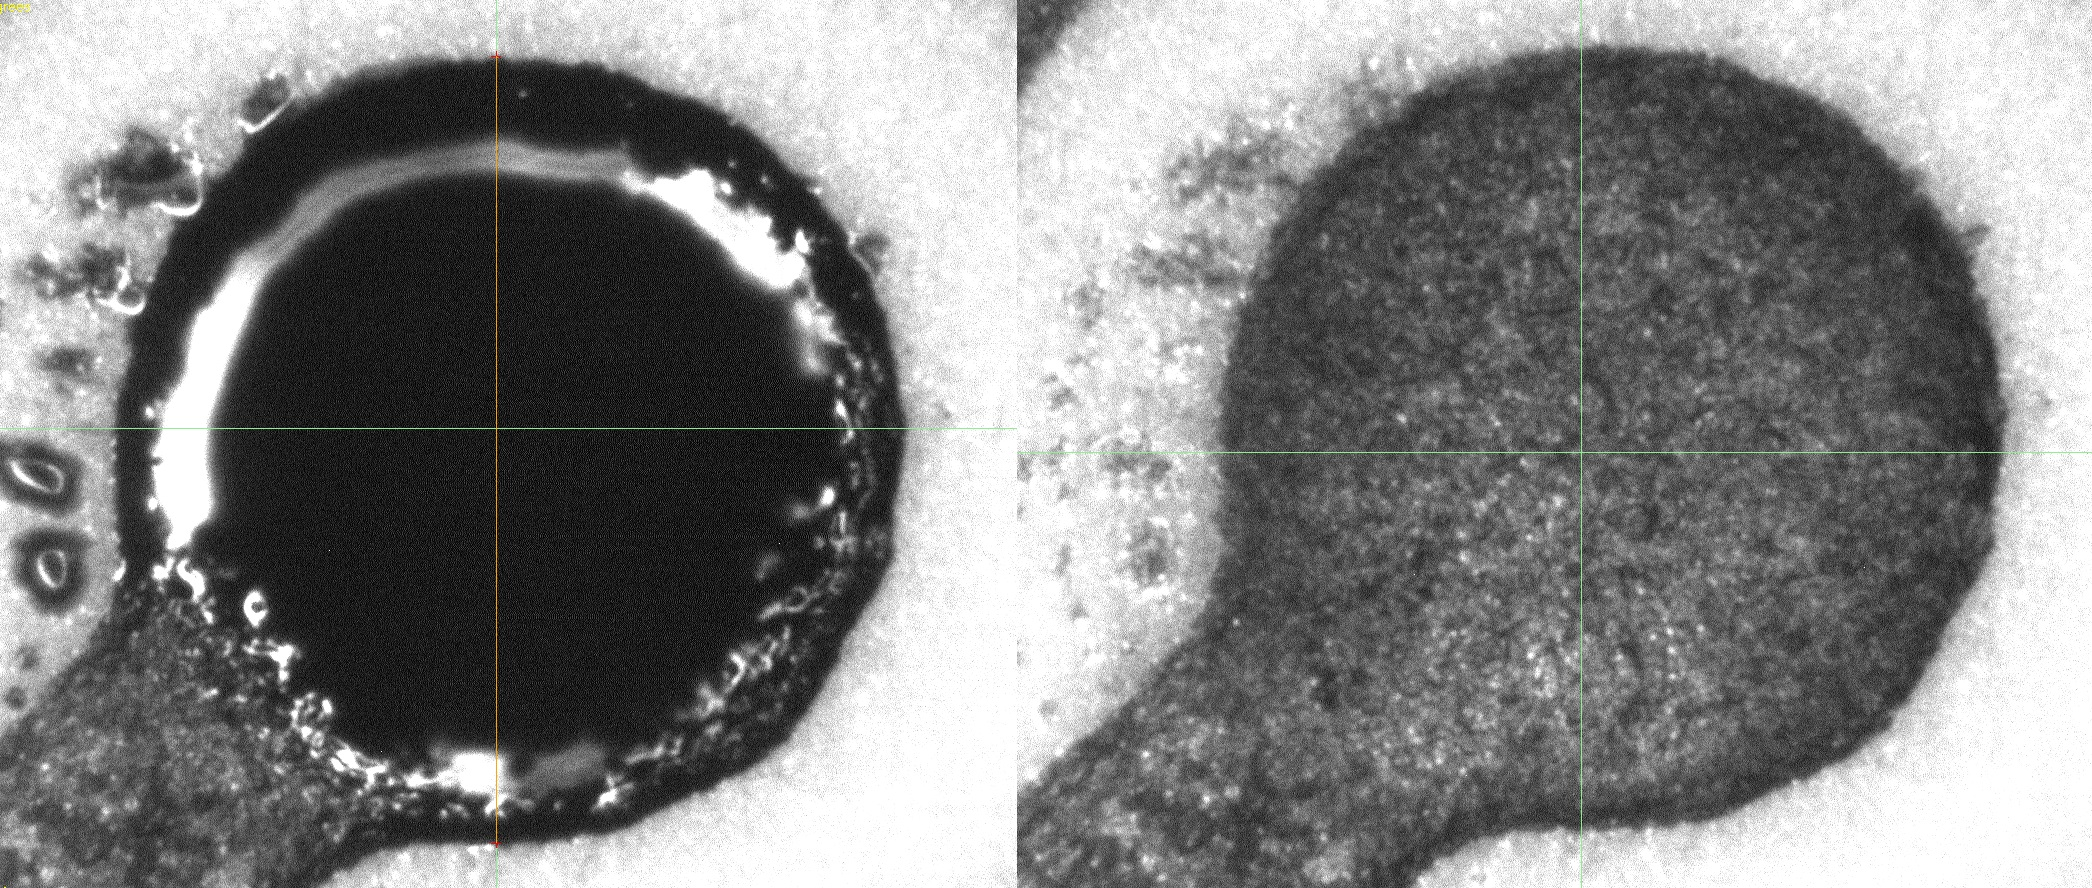
\includegraphics[width=0.5\textwidth]{Figures/Figura_Primera_impresion_circulo}
  \caption{First impression on working electrode (WE1).}
  \label{fig:Figura_Primera_impresion_circulo}
\end{figure}

It is concluded that the average time necessary for drying the ink is 10 minutes. The ink will not be completely dry and anchored until it is cured. For the gold ink curing procedure on \textit{Valox} substrate, a \textit{Hot Plate} is used at 80ºC for 80 minutes (Figure ~\ref{fig:Figura_Hot_Plate}).

\begin{figure}[H]
  \centering
    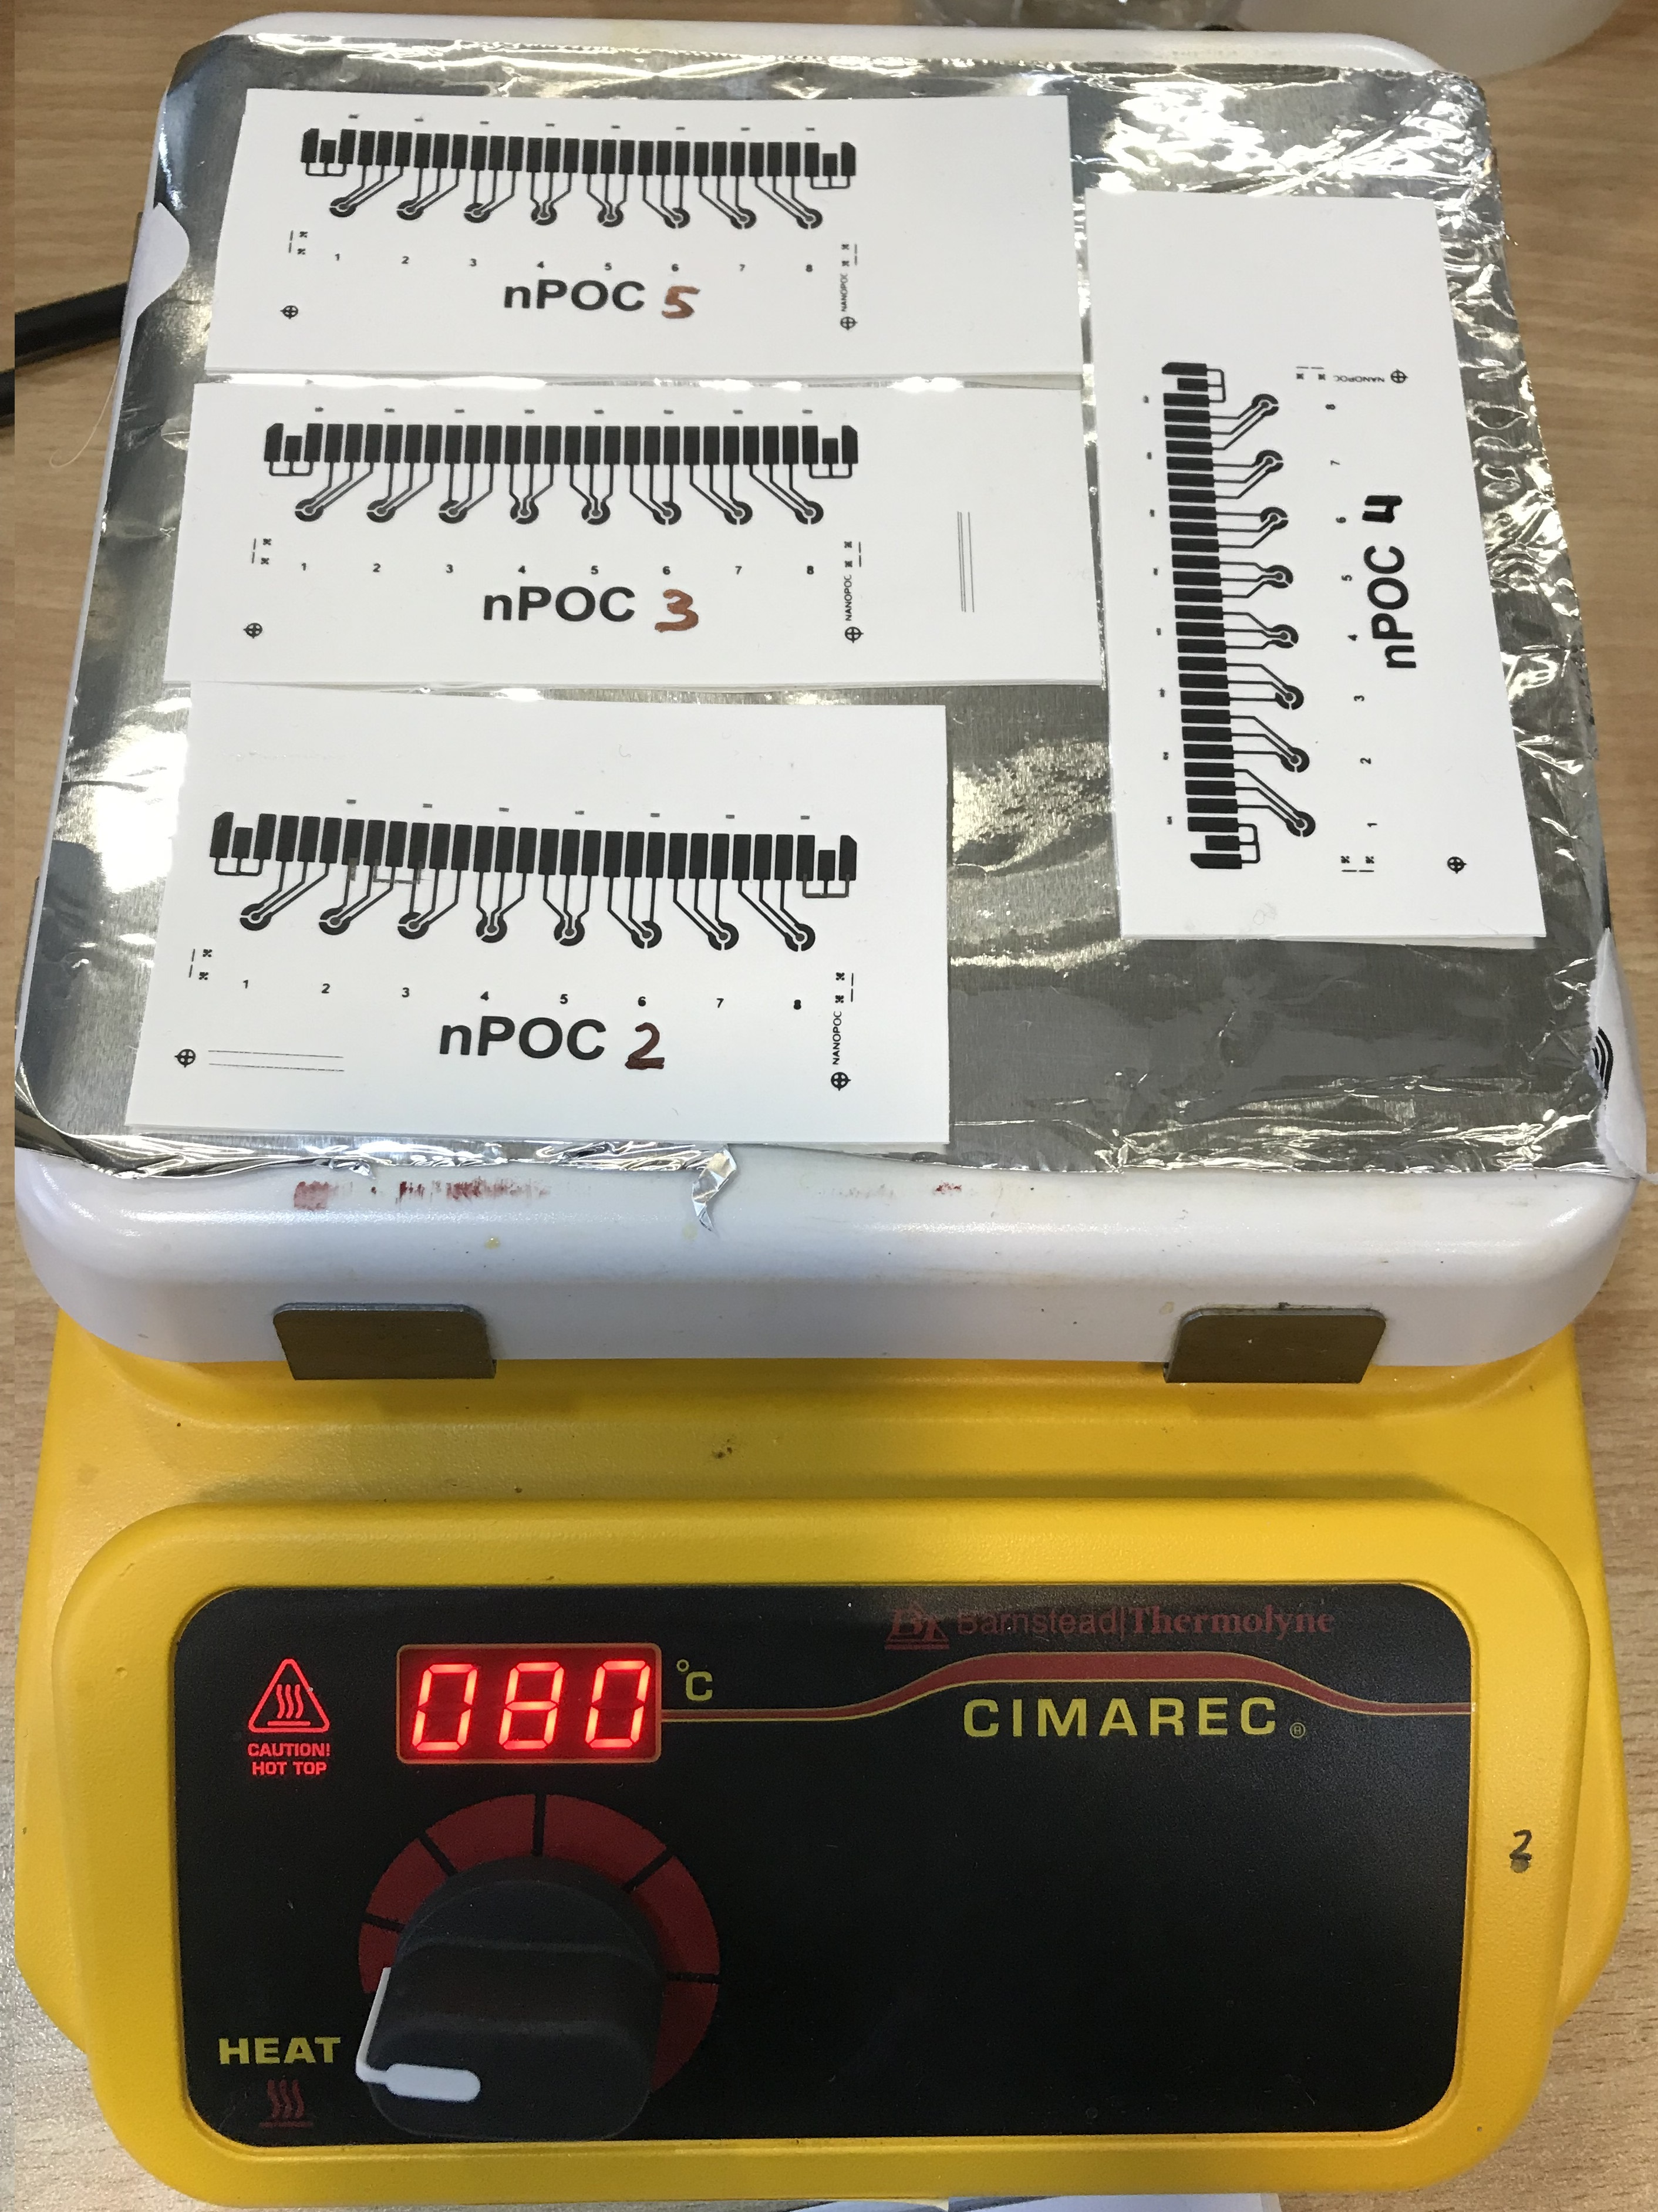
\includegraphics[width=0.4\textwidth]{Figures/Figura_Hot_Plate}
  \caption{\textit{Hot Plate} electrode curing.}
  \label{fig:Figura_Hot_Plate}
\end{figure}

The second printing is made with 1.1 mm diameter circles, to compare the results with the previous work. The 8 working electrodes of the \textit{nPoc5} are printed, one at a time. As can be seen (Figure ~\ref{fig:Figura_Segunda_Impresion_circulo}), the ink that falls on the substrate does not anchor correctly, generating \textit{clusters} of it outside the \emph{WE}.

\begin{figure}[H]
  \centering
    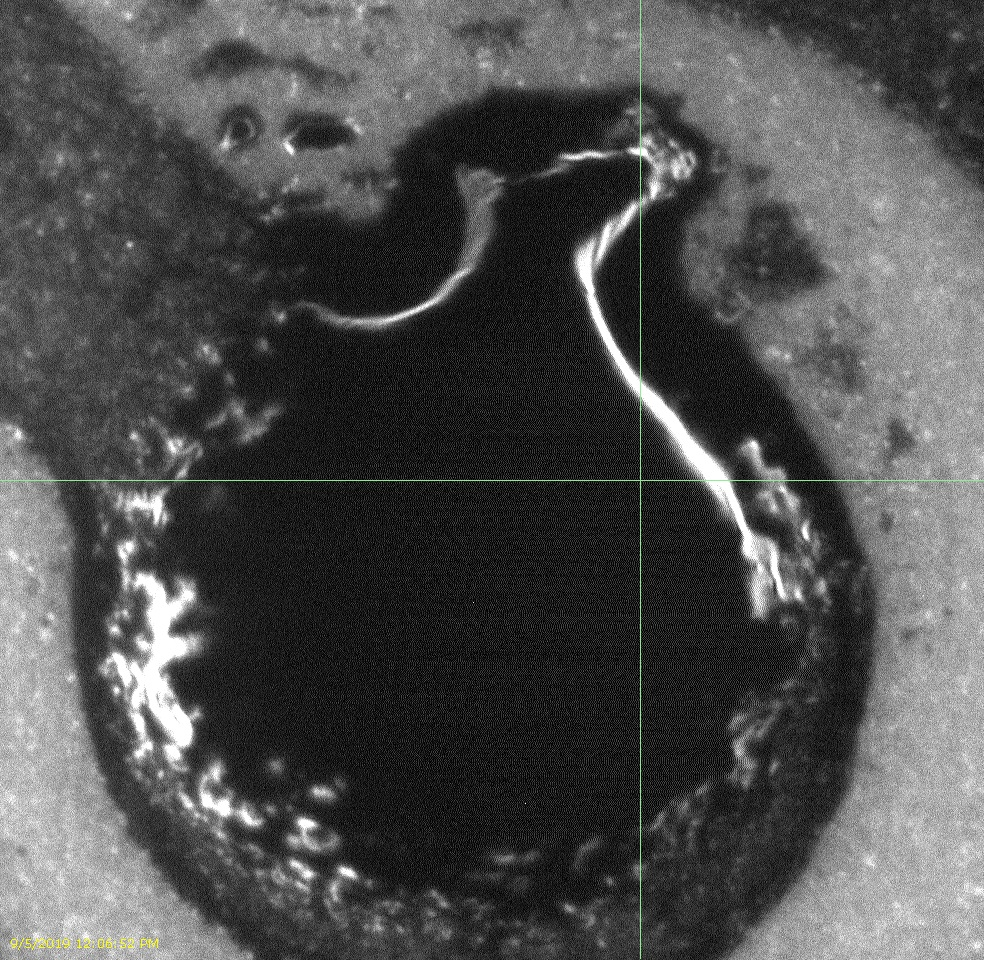
\includegraphics[width=0.45\textwidth]{Figures/Figura_Segunda_Impresion_circulo}
  \caption{1.1 mm circle print on \emph{WE}.}
  \label{fig:Figura_Segunda_Impresion_circulo}
\end{figure}

To increase the level of reproducibility on a larger scale, a pattern of eight circles of 1 mm diameter each is designed. The reference point is centered on the first circle and aligned with the center of the first \emph{WE} of the \textit{nPoc3} substrate.

Slight deviations are noted in the deposition of the gold ink, this may be due to the variations obtained by the screen printing of the carbon ink pattern. However, no significant ink spills are detected on the \textit{Valox} substrate (Figure ~\ref{fig:Figura_impresion_8juntos}).

\begin{figure}[H]
  \centering
    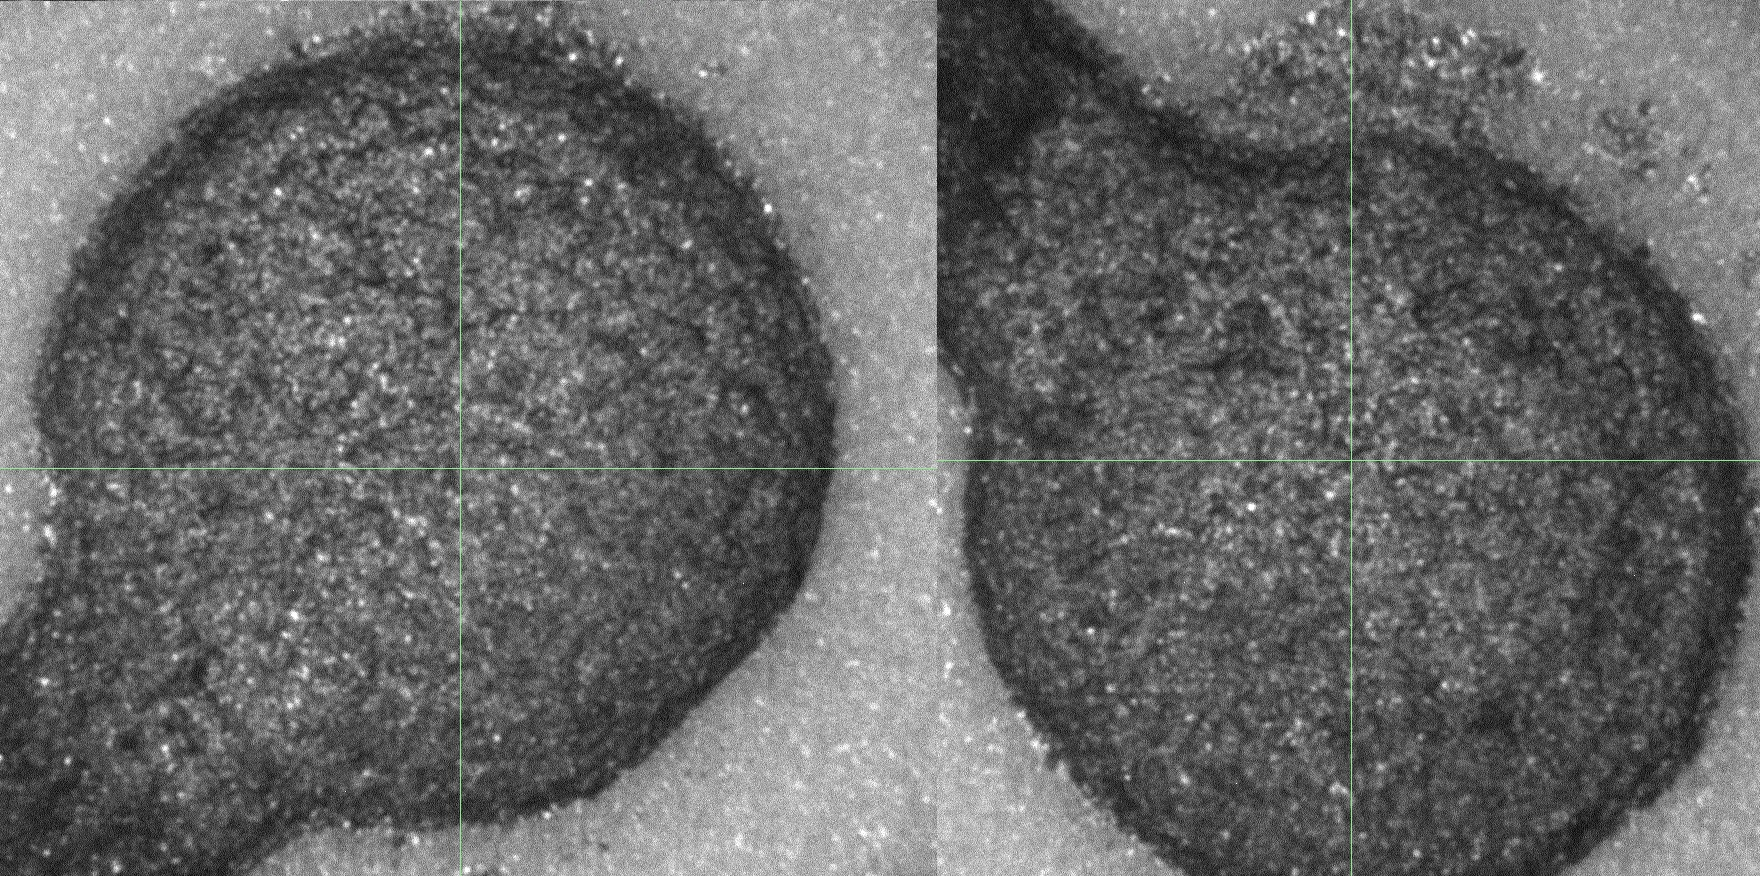
\includegraphics[width=0.6\textwidth]{Figures/Figura_impresion_8juntos}
  \caption{Print comparison between \emph{WE} 3 and 5.}
  \label{fig:Figura_impresion_8juntos}
\end{figure}

The biosensor is then cured on a \textit{Hot Plate} at 80ºC for 80 minutes. The ink is observed to take on a lighter color, similar to the color of pure gold (Figura ~\ref{fig:Figura_impresion_curado}).

\begin{figure}[H]
  \centering
    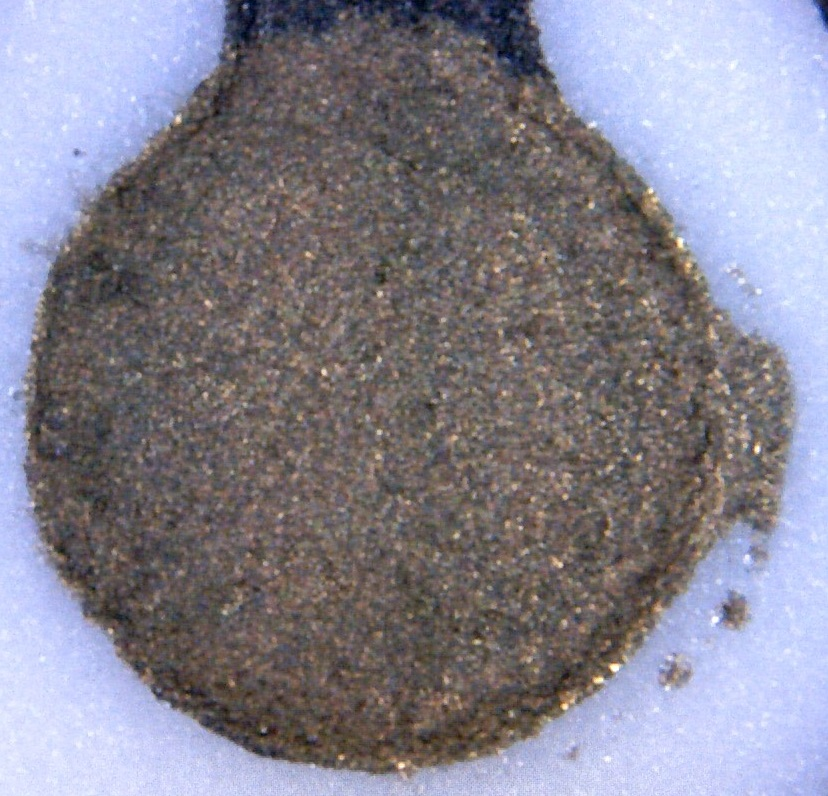
\includegraphics[width=0.45\textwidth]{Figures/Figura_impresion_curado}
  \caption{USB 1000X microscope image of \emph{WE} cured in \textit{Hot Plate}.}
  \label{fig:Figura_impresion_curado}
\end{figure}

For electrical characterization, a pattern was designed in the form of the connection between two test contacts of the biosensor (Figure ~\ref{fig:Figura_contactos_prueba}).

\begin{figure}[H]
  \centering
    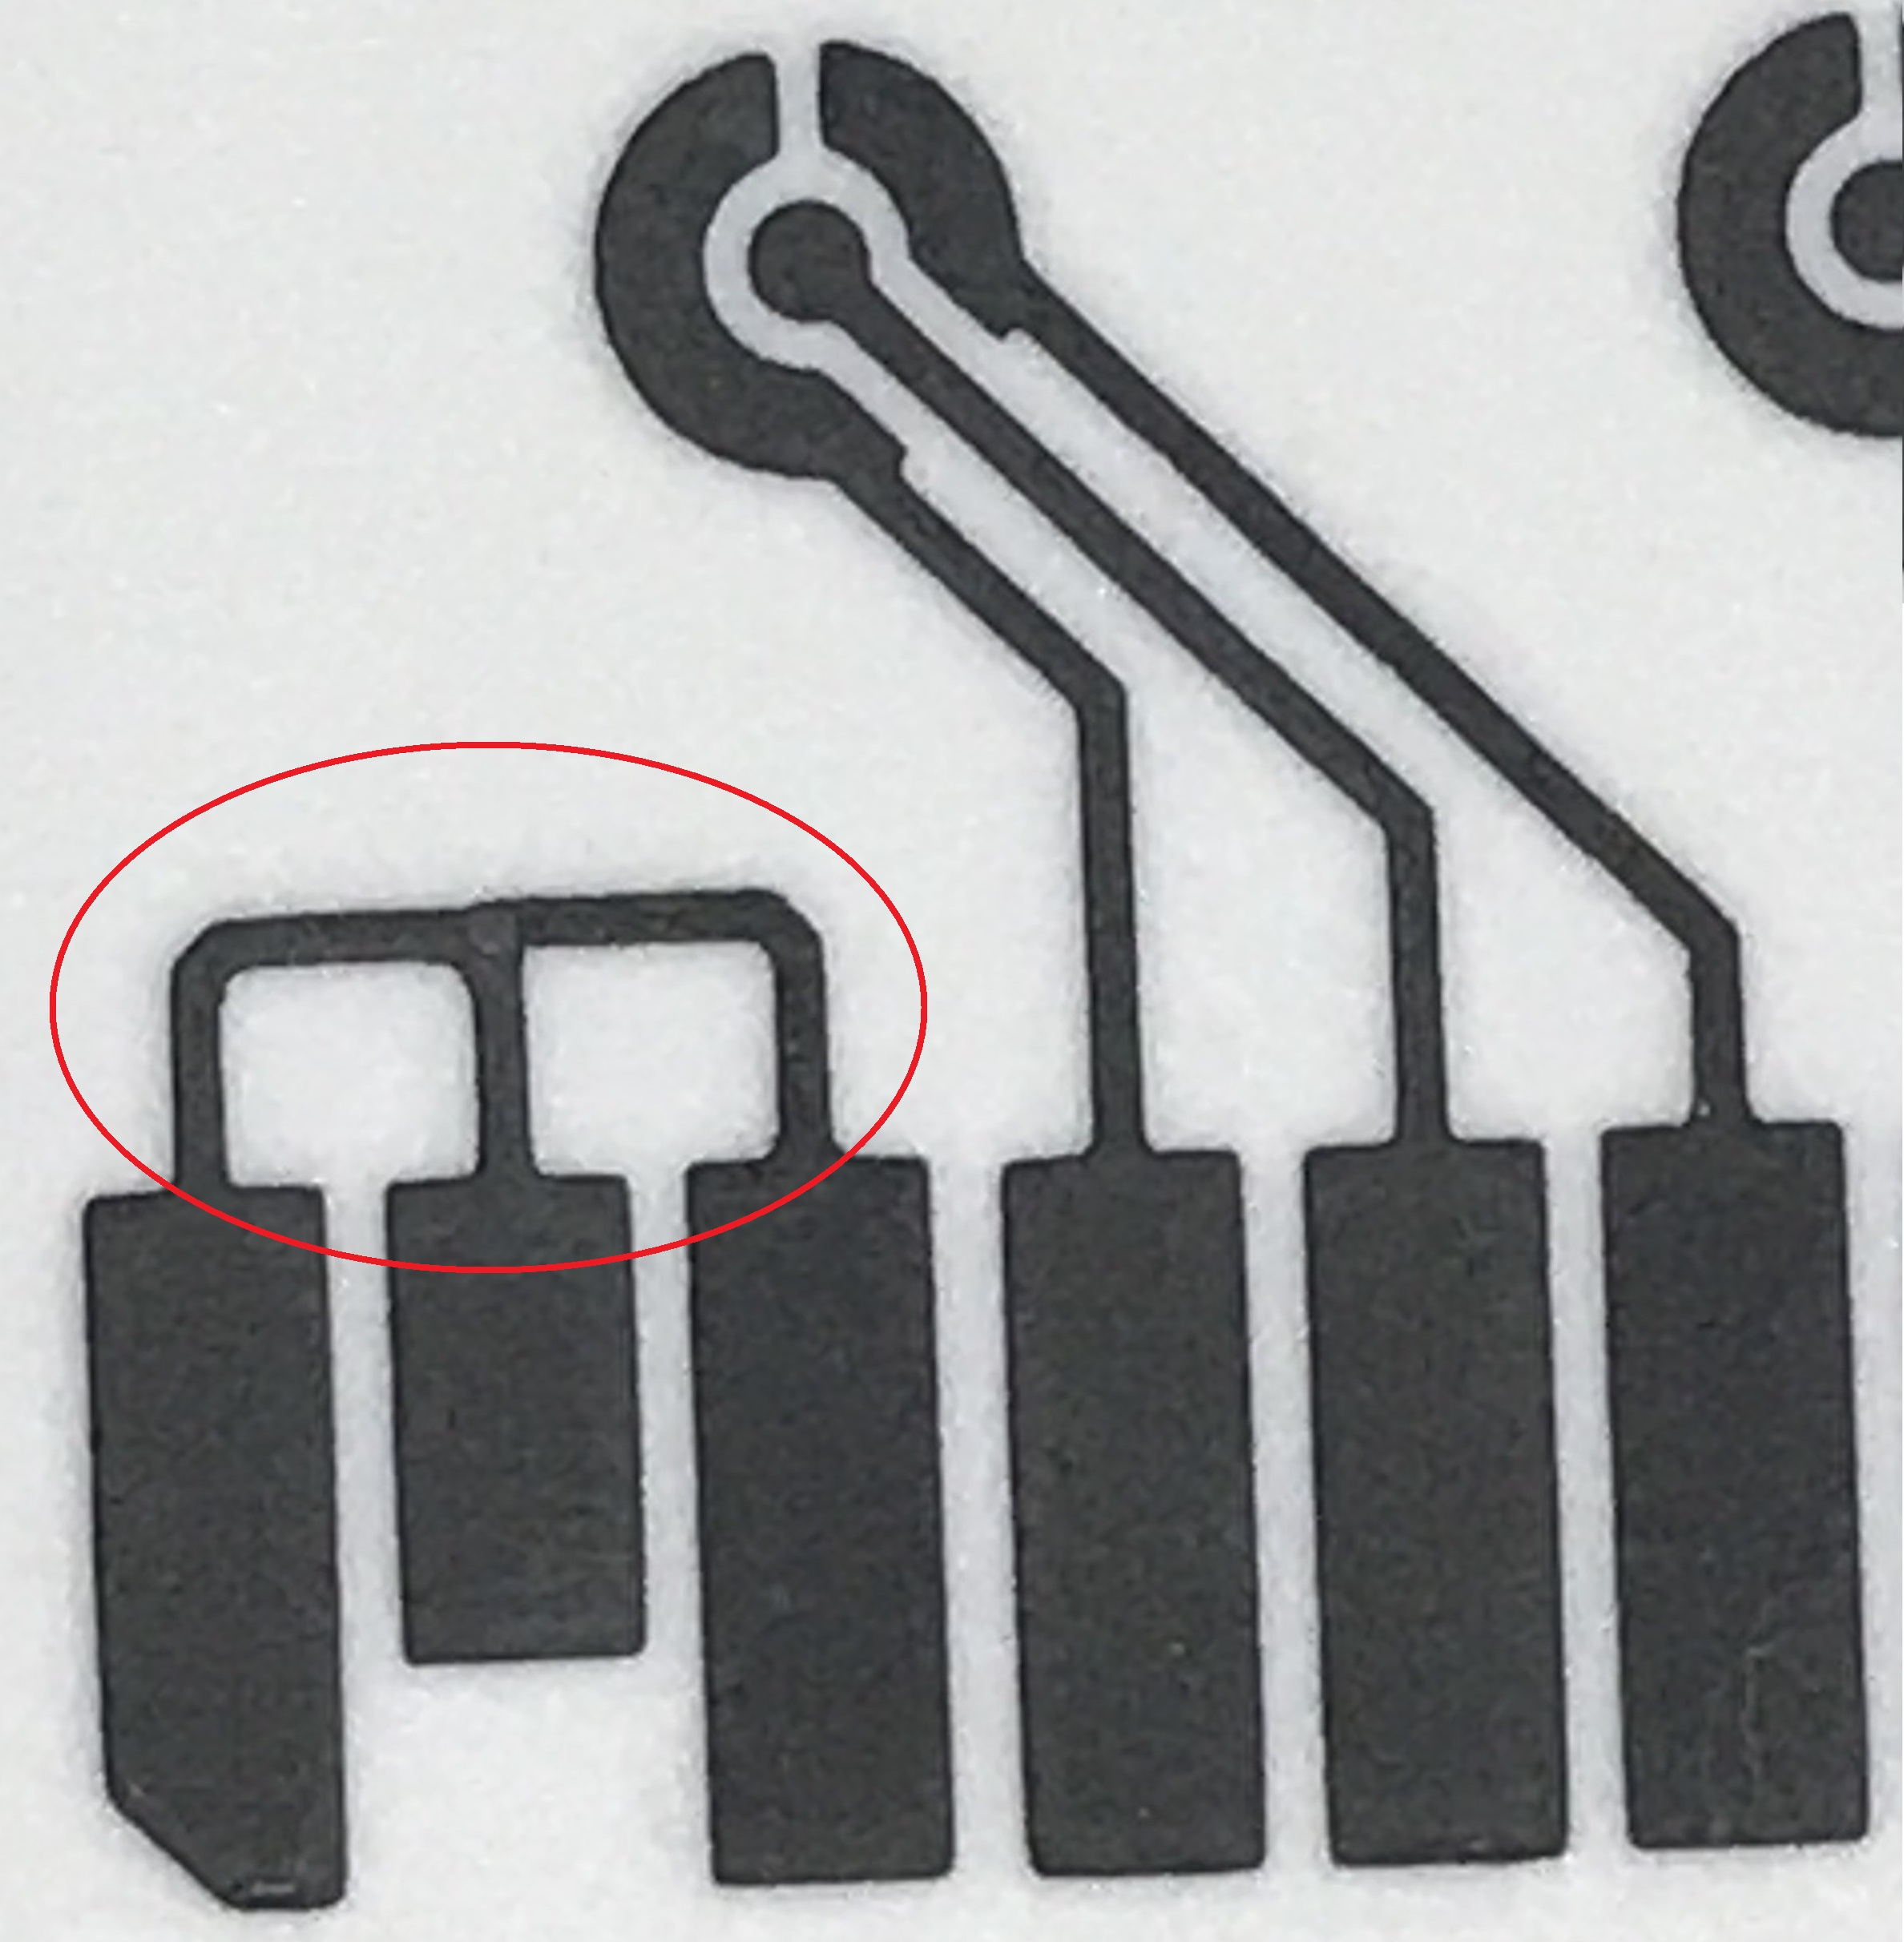
\includegraphics[width=0.45\textwidth]{Figures/Figura_contactos_prueba}
  \caption{Test contacts in biosensor.}
  \label{fig:Figura_contactos_prueba}
\end{figure}

The design is 2.5 mm high and 5.5 mm long, the path width is 0.4 mm. For this impression, no reference point was used, but the impression origin point was aligned with the beginning of the carbon pathways. An extra of 1 mm was added over the contacts for a better carbon-gold nanoparticle ratio. Given the good anchorage of the gold nanoparticle ink on the carbon, the desired design was obtained correctly, almost without spills (Figure ~\ref{fig:Figura_contactos_prueba_con_Oro}). Two layers of the design were printed, both cured on \textit{Hot Plate} at 80°C for 80 minutes.

\begin{figure}[H]
  \centering
    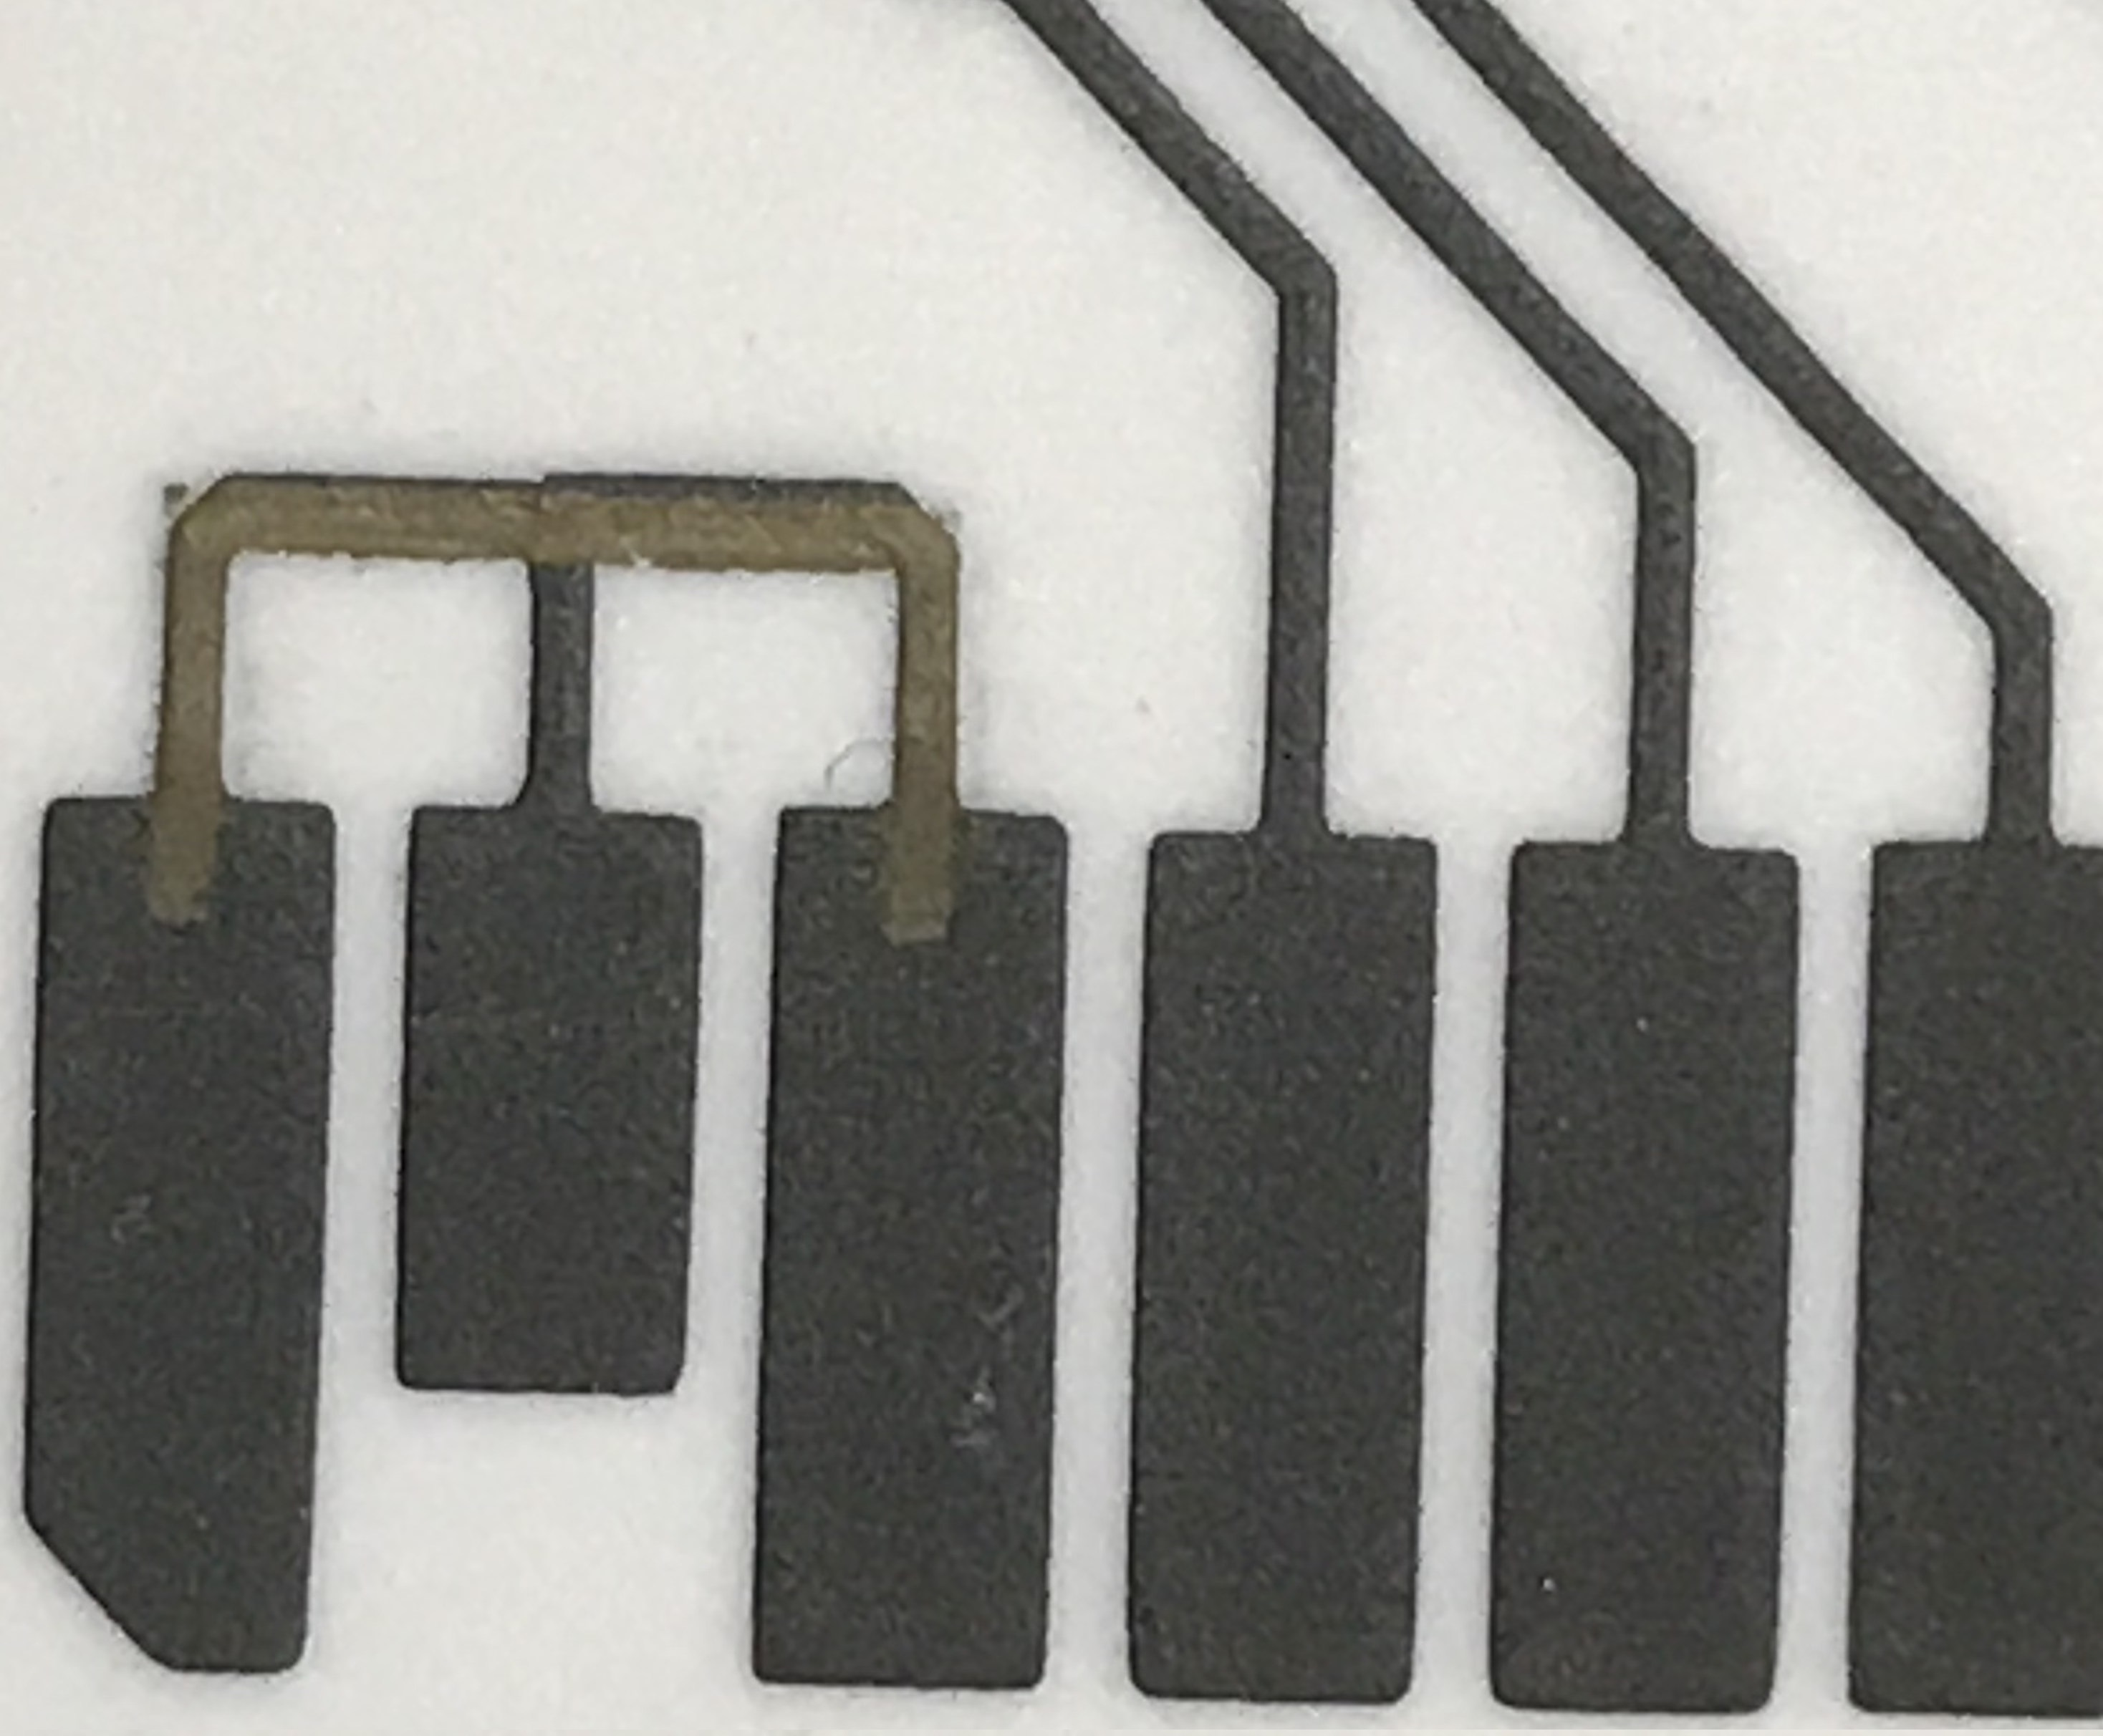
\includegraphics[width=0.45\textwidth]{Figures/Figura_contactos_prueba_con_Oro}
  \caption{Test contacts with printed gold nanoparticles ink.}
  \label{fig:Figura_contactos_prueba_con_Oro}
\end{figure}

In order to have a greater amount of tests in the electrochemical characterization, prints were made with gold nanoparticle ink on \textit{Valox} substrate, without carbon ink (Figure ~\ref{fig:Figura_impresion_sustrato_valox_tinta_Oro}), on a PET (Polyethylene Terephthalate) substrate and a cellulose pulp sheet (conventional notebook sheet).

\begin{figure}[H]
  \centering
    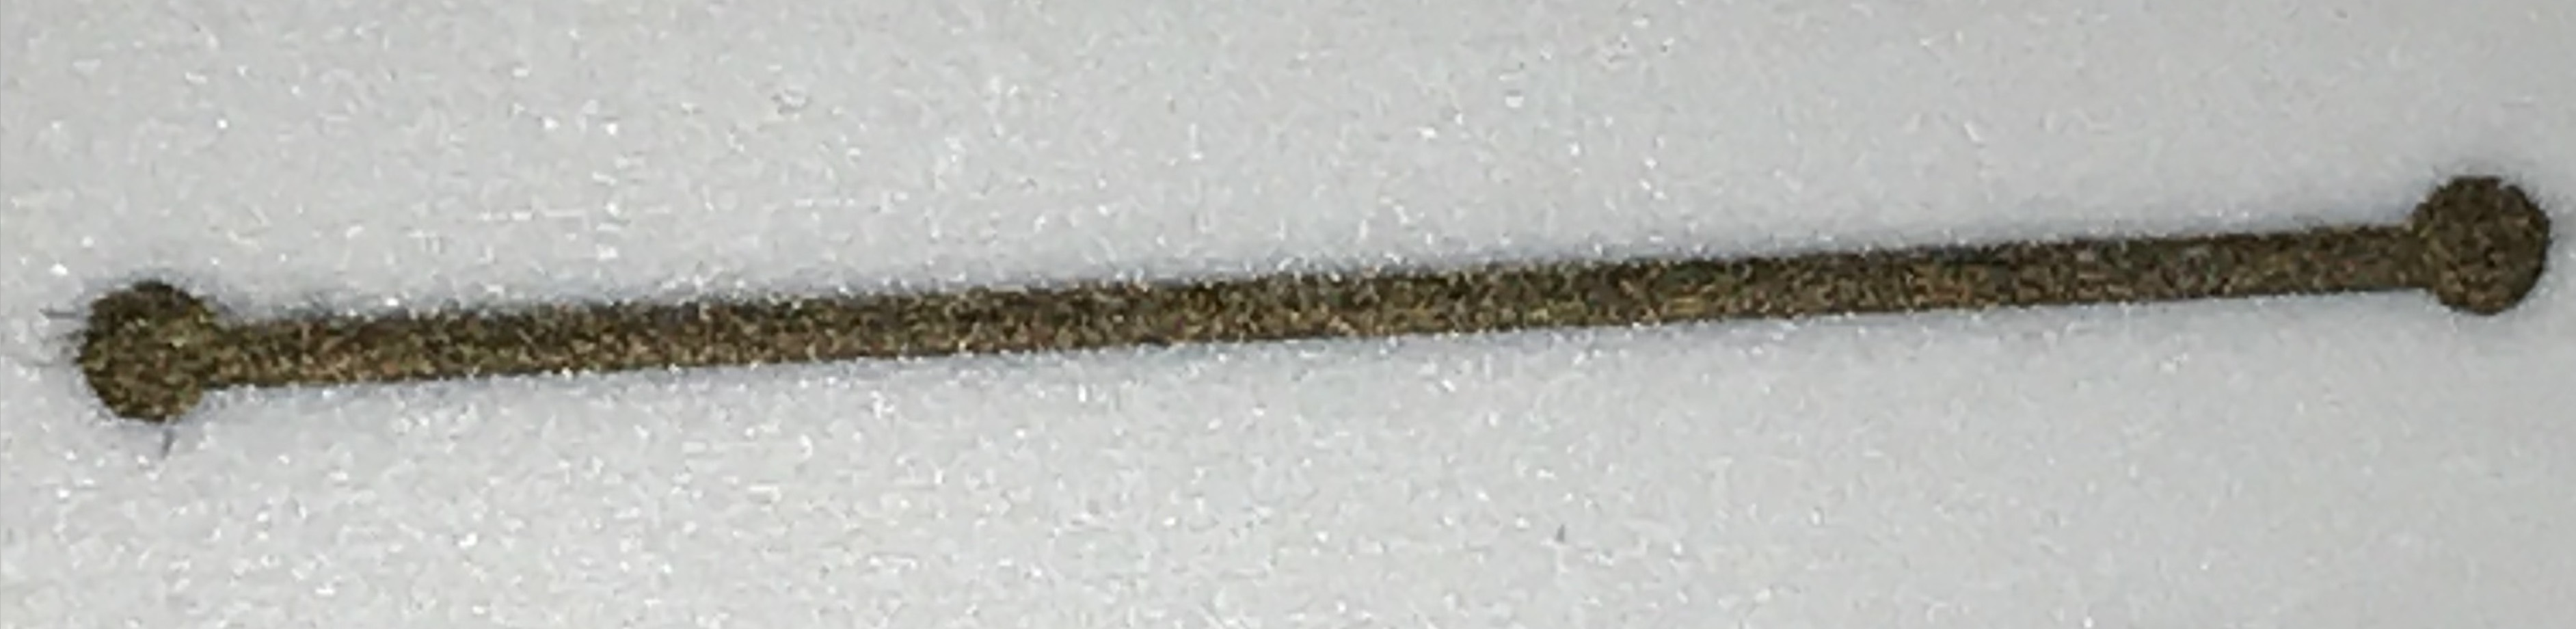
\includegraphics[width=0.5\textwidth]{Figures/Figura_impresion_sustrato_valox_tinta_Oro}
  \caption{Printing on \textit{Valox} substrate.}
  \label{fig:Figura_impresion_sustrato_valox_tinta_Oro}
\end{figure}

Two circles of 1 mm diameter separated 16 mm were printed on the \textit{Valox} substrate and the cellulose pulp sheet, which were then joined by a line 17 mm long and 0.4 mm wide, thus the ink was printed from half a circle to half the other, ensuring the continuity of the material. Two identical layers were printed, for the \textit{Valox} substrate a cure was made between each impression in \textit{Hot Plate} at 80ºC for 80 minutes.

A different design was made for the PET substrate (Figure ~\ref{fig:Figura_impresion_sobre_PET}) because there was no reference to how the ink would anchor on the base. An arrangement of six drawings was made in two columns, composed of two squares of 1 mm side separated 16 mm and a bar 17 mm long and 0.4 mm wide. The separation between columns is 65 mm and 20 mm between rows. The separation into columns is due to the fact that half of the substrate was cleaned with ethyl alcohol, in this way, will be observed the differences between the treated and untreated substrate. Two identical layers were printed with their respective cures on \textit{Hot Plate} at 80°C for 80 minutes.

\begin{figure}[H]
  \centering
    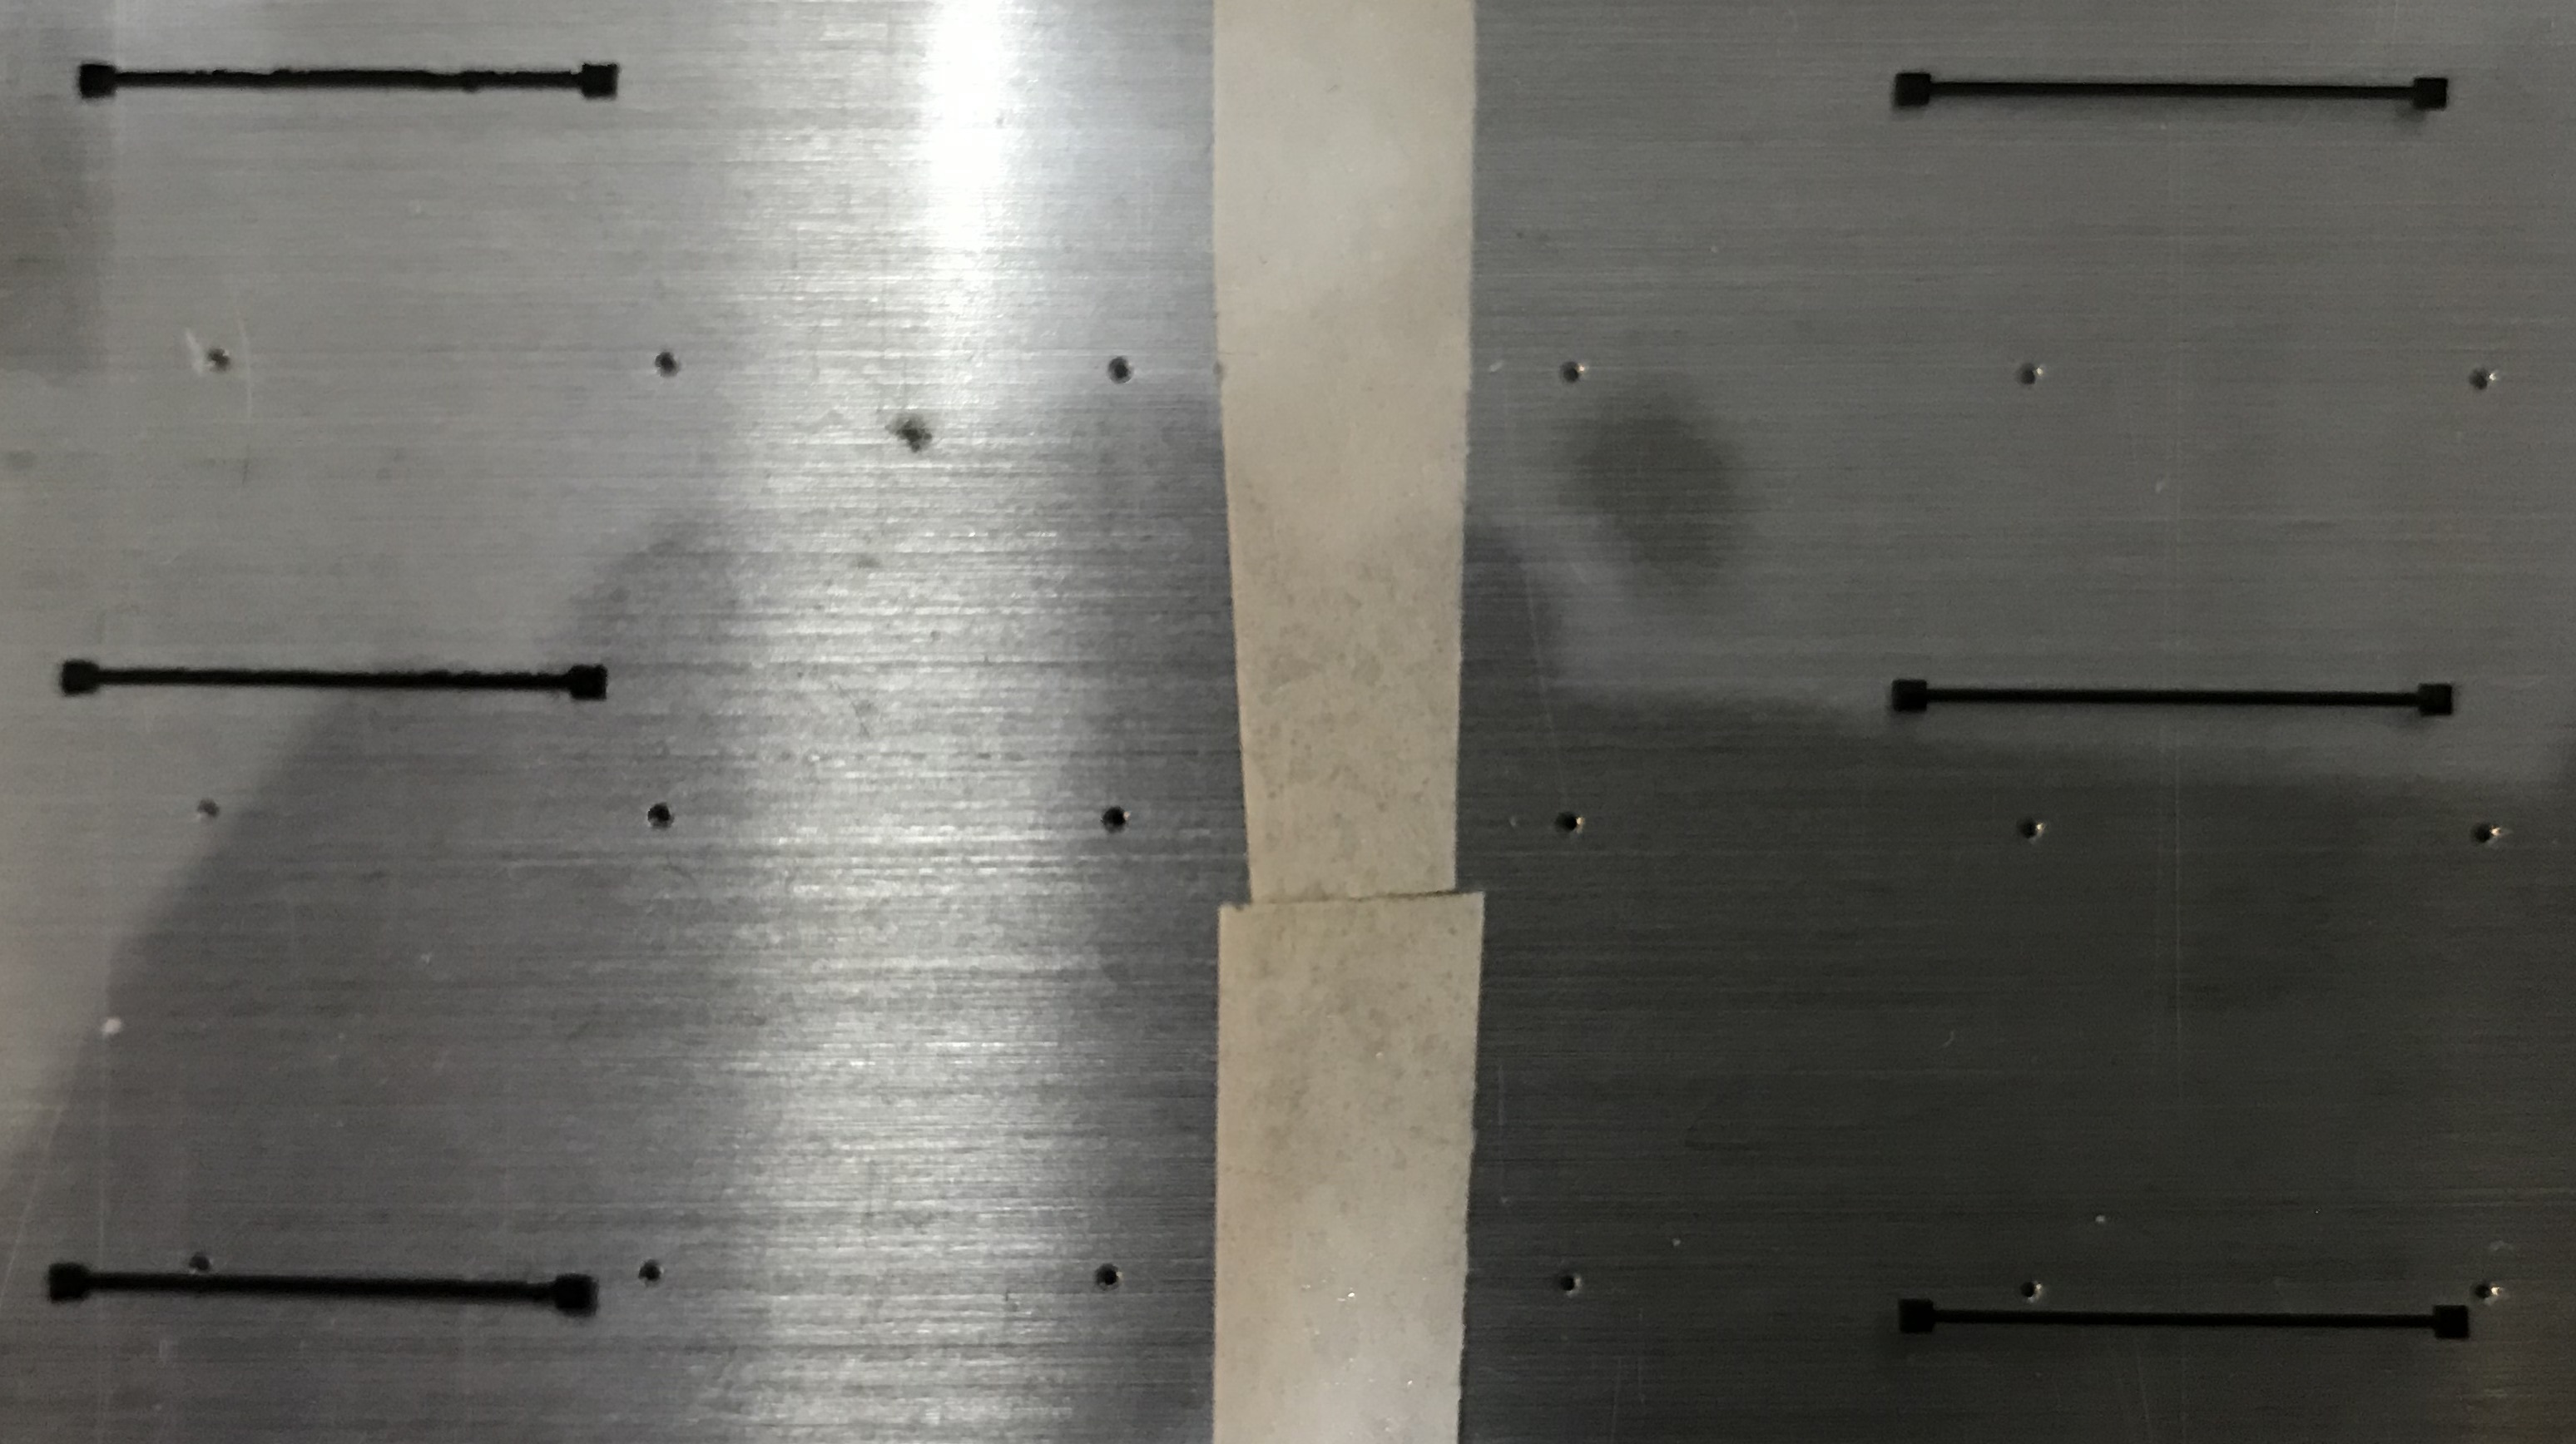
\includegraphics[width=0.5\textwidth]{Figures/Figura_impresion_sobre_PET}
  \caption{Printed design on PET substrate.}
  \label{fig:Figura_impresion_sobre_PET}
\end{figure}

\section{Characterizations}
\subsection{Electrical characterization}
The electrical characterization consists of the 4-tip resistance measurement, explained earlier in Chapter 2, \hyperref[subsec:carac_elec]{section 2.3.1}. The resistance measurements were made on carbon ink, carbon ink plus one layer, and two layers of cured gold nanoparticles ink.

It should be noted that the results obtained from this measurement is made up of an electrical parallel between the resistance of the carbon ink and the resistance of the gold nanoparticles ink. A considerable decrease in resistance was obtained (compared to a parallel of two carbon resistors) in accordance with the proposed theory, since the resistivity of gold (2.44·10\textsuperscript{-8} Ohm·m) is much lower than that of carbon (3.5·10\textsuperscript{-5} Ohm·m) \cite{Resistividad}.

\subsection{Dimensional characterization}
For the dimensional characterization the fiducial camera of the \textit{Dimatix} printer was used, obtaining the dimensions of the \emph{WE} and the separations between it, the \emph{CE} and the \emph{RE} (Figure ~\ref{fig:Figura_medicion_WE}).

\begin{figure}[H]
  \centering
    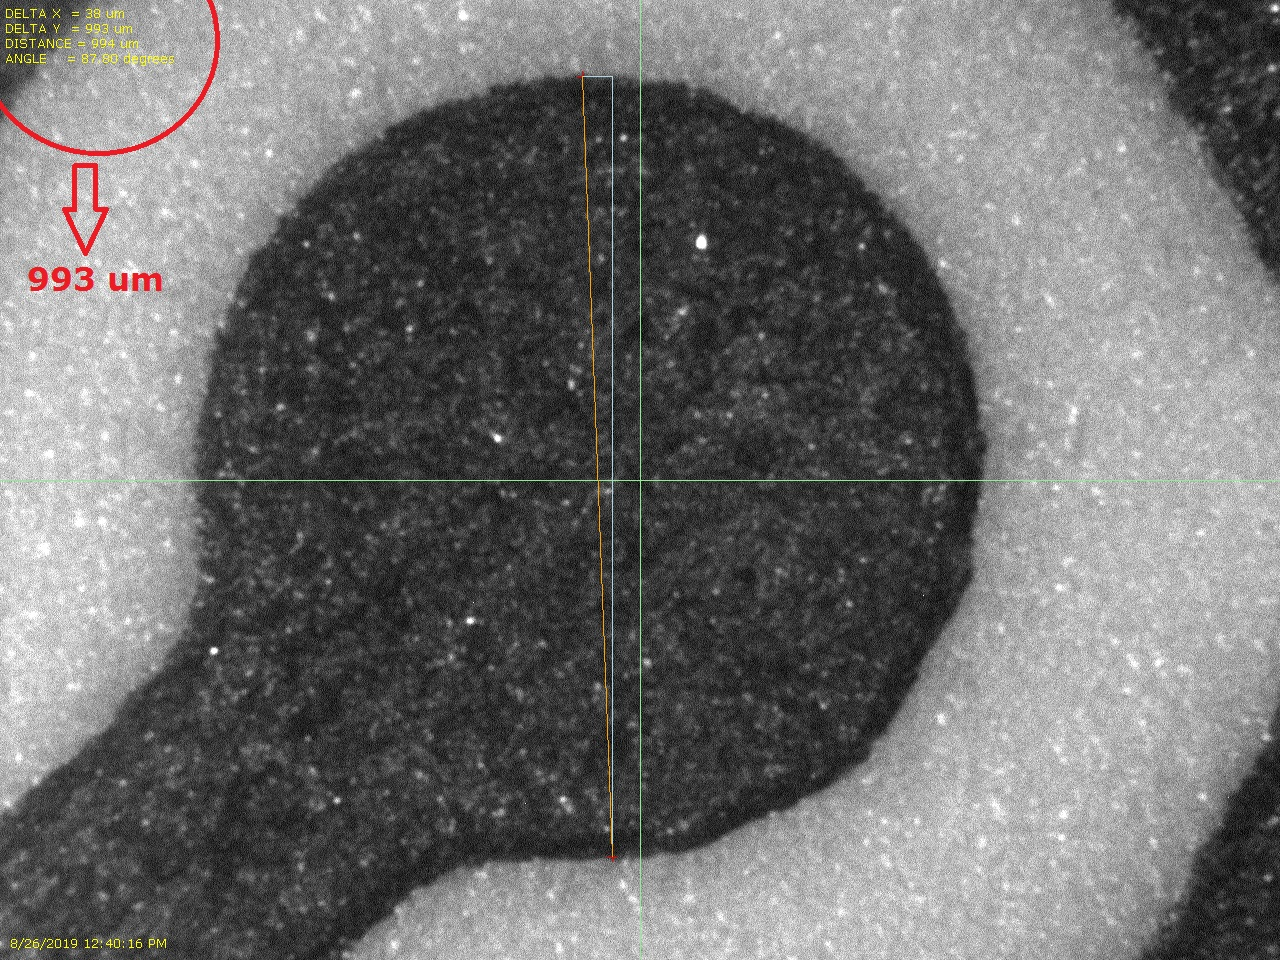
\includegraphics[width=0.5\textwidth]{Figures/Figura_medicion_WE}
  \caption{\emph{WE} diameter measurement.}
  \label{fig:Figura_medicion_WE}
\end{figure}

The roughness and thickness of the carbon film and the film obtained with the gold nanoparticles ink were obtained using a \textit{Bruker} model \textit{Dektak XT} contact profilometer with a 12.5 $\mu$m \textit{Stylus} tip (Figure ~\ref{fig:Figura_Perfilometro}). The force applied by the tip was in both cases 3 mgf.

\begin{figure}[H]
  \centering
    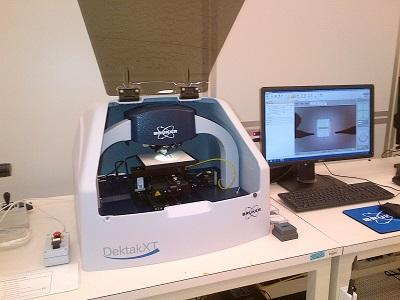
\includegraphics[width=0.5\textwidth]{Figures/Figura_Perfilometro}
  \caption{Dektak XT Advanced Profilometer.}
  \label{fig:Figura_Perfilometro}
\end{figure}

For this characterization, a 2000 $\mu$m path was determined on the working electrode for 15 seconds and then the area of interest was selected to measure the roughness. Three values were taken on the entire sample:

$\bullet$ The average value of maximum roughness (Rz).

$\bullet$ The highest peak roughness (Rt).

$\bullet$ The average roughness value (Ra).
\\

To characterize the thickness of the \emph{WE}, a path of 1000 $\mu$m was set for 15 seconds. The length of the route was determined at that value in order to obtain the rise/fall steps and with this obtain a reference (Figure ~\ref{fig:Figura_grafico_perfilometro}). To determine the thickness of the gold ink, the thickness of a carbon pad and that of a \emph{WE} with gold nanoparticles ink were measured. Making the difference between the two, the thickness of two layers of gold ink printed by \textit{Inkjet} was obtained.

\begin{figure}[H]
  \centering
    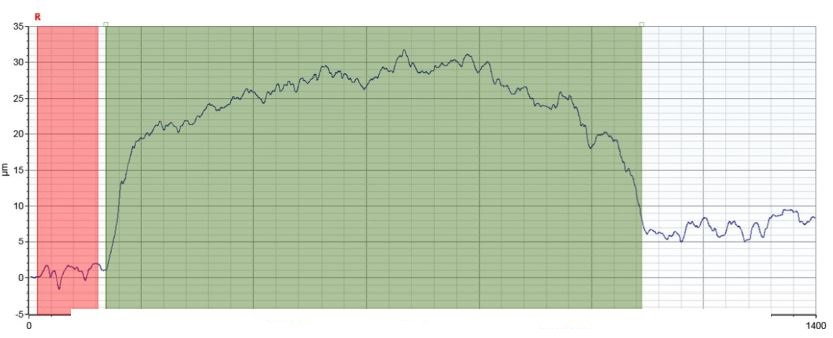
\includegraphics[width=0.8\textwidth]{Figures/Figura_grafico_perfilometro}
  \caption{Thickness characterization graph.}
  \label{fig:Figura_grafico_perfilometro}
\end{figure}

For these studies, two samples were used, identified as nPoc3 and nPoc5 cartridges, having two cured layers of 1 mm and 1.1 mm in diameter (Gold nanoparticles ink) respectively. From each one, the working electrodes identified as 3 and 4 were used to obtain a varied sampling. Two measurements were made on each and then averaged.

\subsection{Electrochemical characterization}
The electrochemical characterization was carried out on different configurations of substrates and inks to obtain multiple comparisons of interest for the project. Samples are listed in test order (Figure ~\ref{fig:Figura_pruebas_muestras}):

$\bullet$ Gold thin film electrode deposited by sputtering on silicon. (Figure ~\ref{fig:Figura_pruebas_muestras} (a))

$\bullet$ Screen printed carbon film electrode on \textit{Valox} substrate. (Figure ~\ref{fig:Figura_pruebas_muestras} (b))

$\bullet$ Screen printed carbon film electrode and inkjet printed gold nanoparticles ink of 1 mm diameter on \textit{Valox} substrate. (Figure ~\ref{fig:Figura_pruebas_muestras} (c))

$\bullet$ Screen printed carbon film electrode and inkjet printed gold nanoparticles ink of 1.1 mm diameter on \textit{Valox} substrate.

$\bullet$ Inkjet printed gold nanoparticles ink on \textit{Valox} substrate.

$\bullet$ Inkjet printed gold nanoparticles ink on PET substrate. (Figure ~\ref{fig:Figura_pruebas_muestras} (d))

$\bullet$ Inkjet printed gold nanoparticles ink on cellulose pulp substrate. (Figure ~\ref{fig:Figura_pruebas_muestras} (e))

\begin{figure}[H]
  \centering
    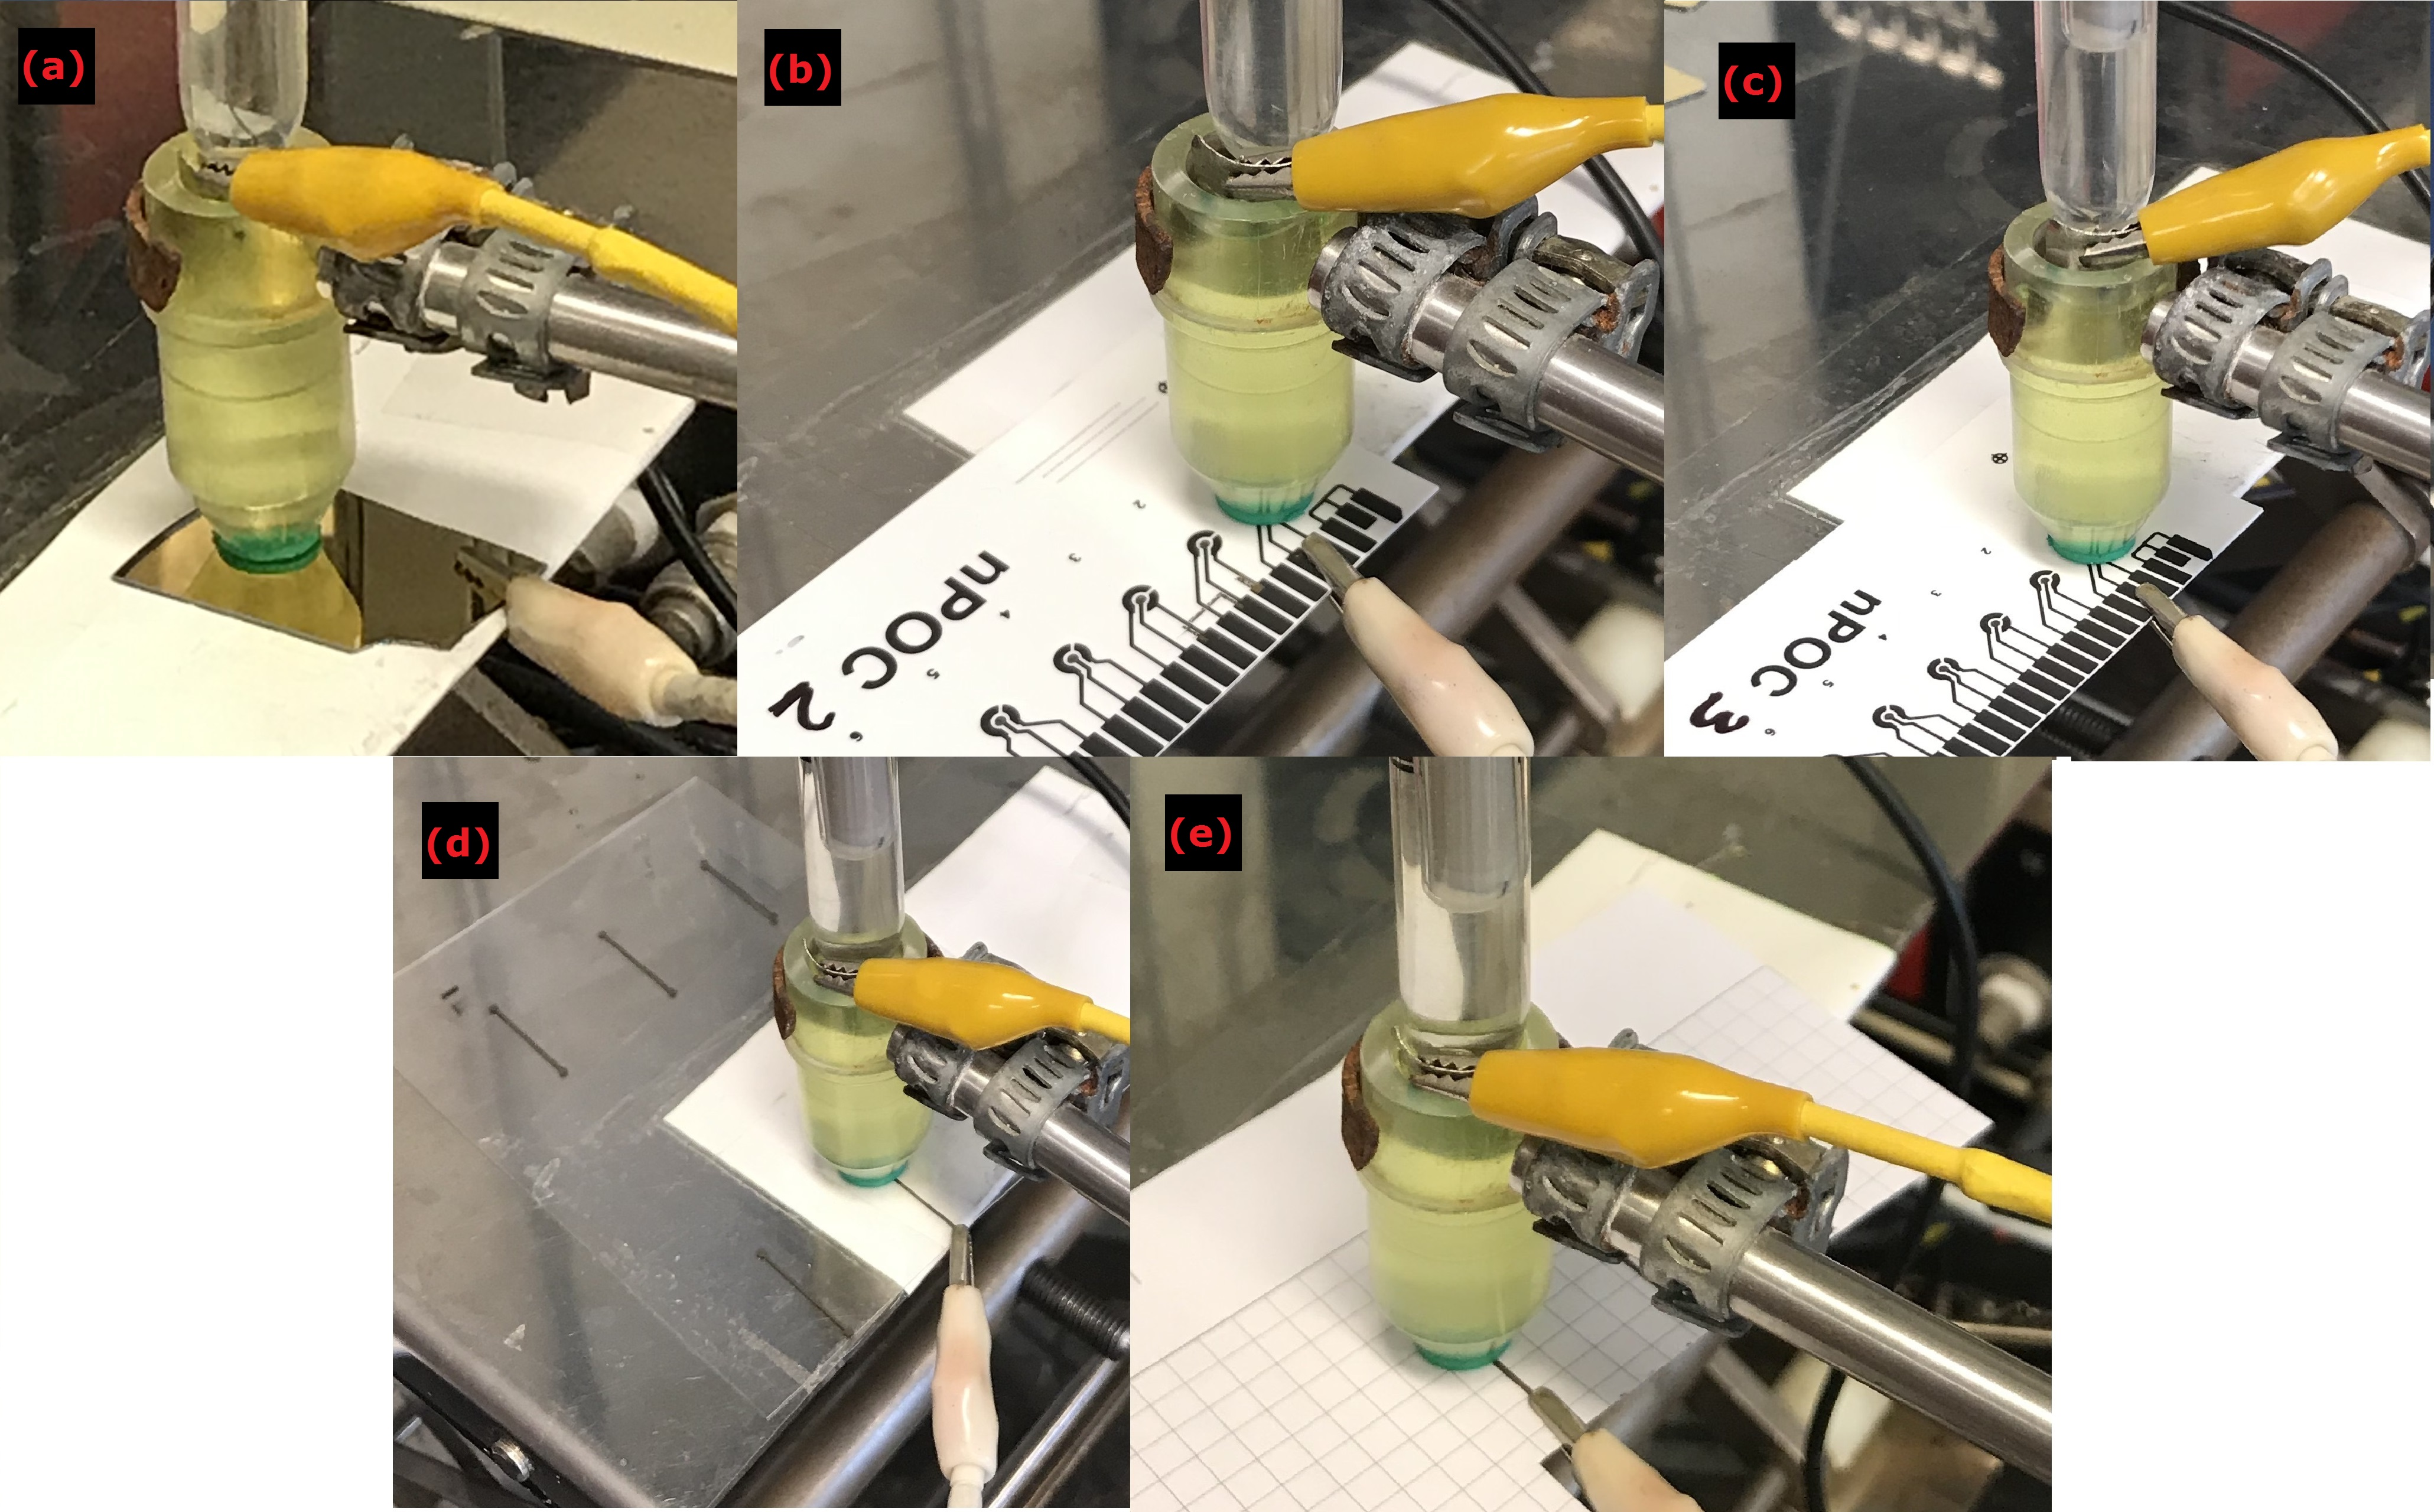
\includegraphics[width=1\textwidth]{Figures/Figura_pruebas_muestras}
  \caption{Samples where the electrochemical characterization was carried out.}
  \label{fig:Figura_pruebas_muestras}
\end{figure}
To make the tests comparable to each other, a 2 cm\textsuperscript{2} area platinum counter electrode and a \textit{Cole-Parmer} reference mercury(I) chloride or saturated \textit{Calomel} (Hg\textsubscript{2}Cl\textsubscript{2}) electrode were used, both external to the samples. The electrochemical cell reservoir was made of acrylic with an approximate volume of 3 ml. It has a hole at the bottom where polypropylene seals can be placed. In the experiments a 1 mm diameter seal was used, to have the same geometric area of 0.785 mm\textsuperscript{2} in all the tests.

After contacting the seal with the electrode, the cell is filled from the top with the ferrocyanide (K\textsubscript{4}Fe(CN)\textsubscript{6}) and ferricyanide (K\textsubscript{3}Fe(CN)\textsubscript{6}) probe solution and the supporting electrolyte of potassium chloride (KCl). It was verified that there were no leaks (Figure ~\ref{fig:Figura_prueba_electroquimica}).

\begin{figure}[H]
  \centering
    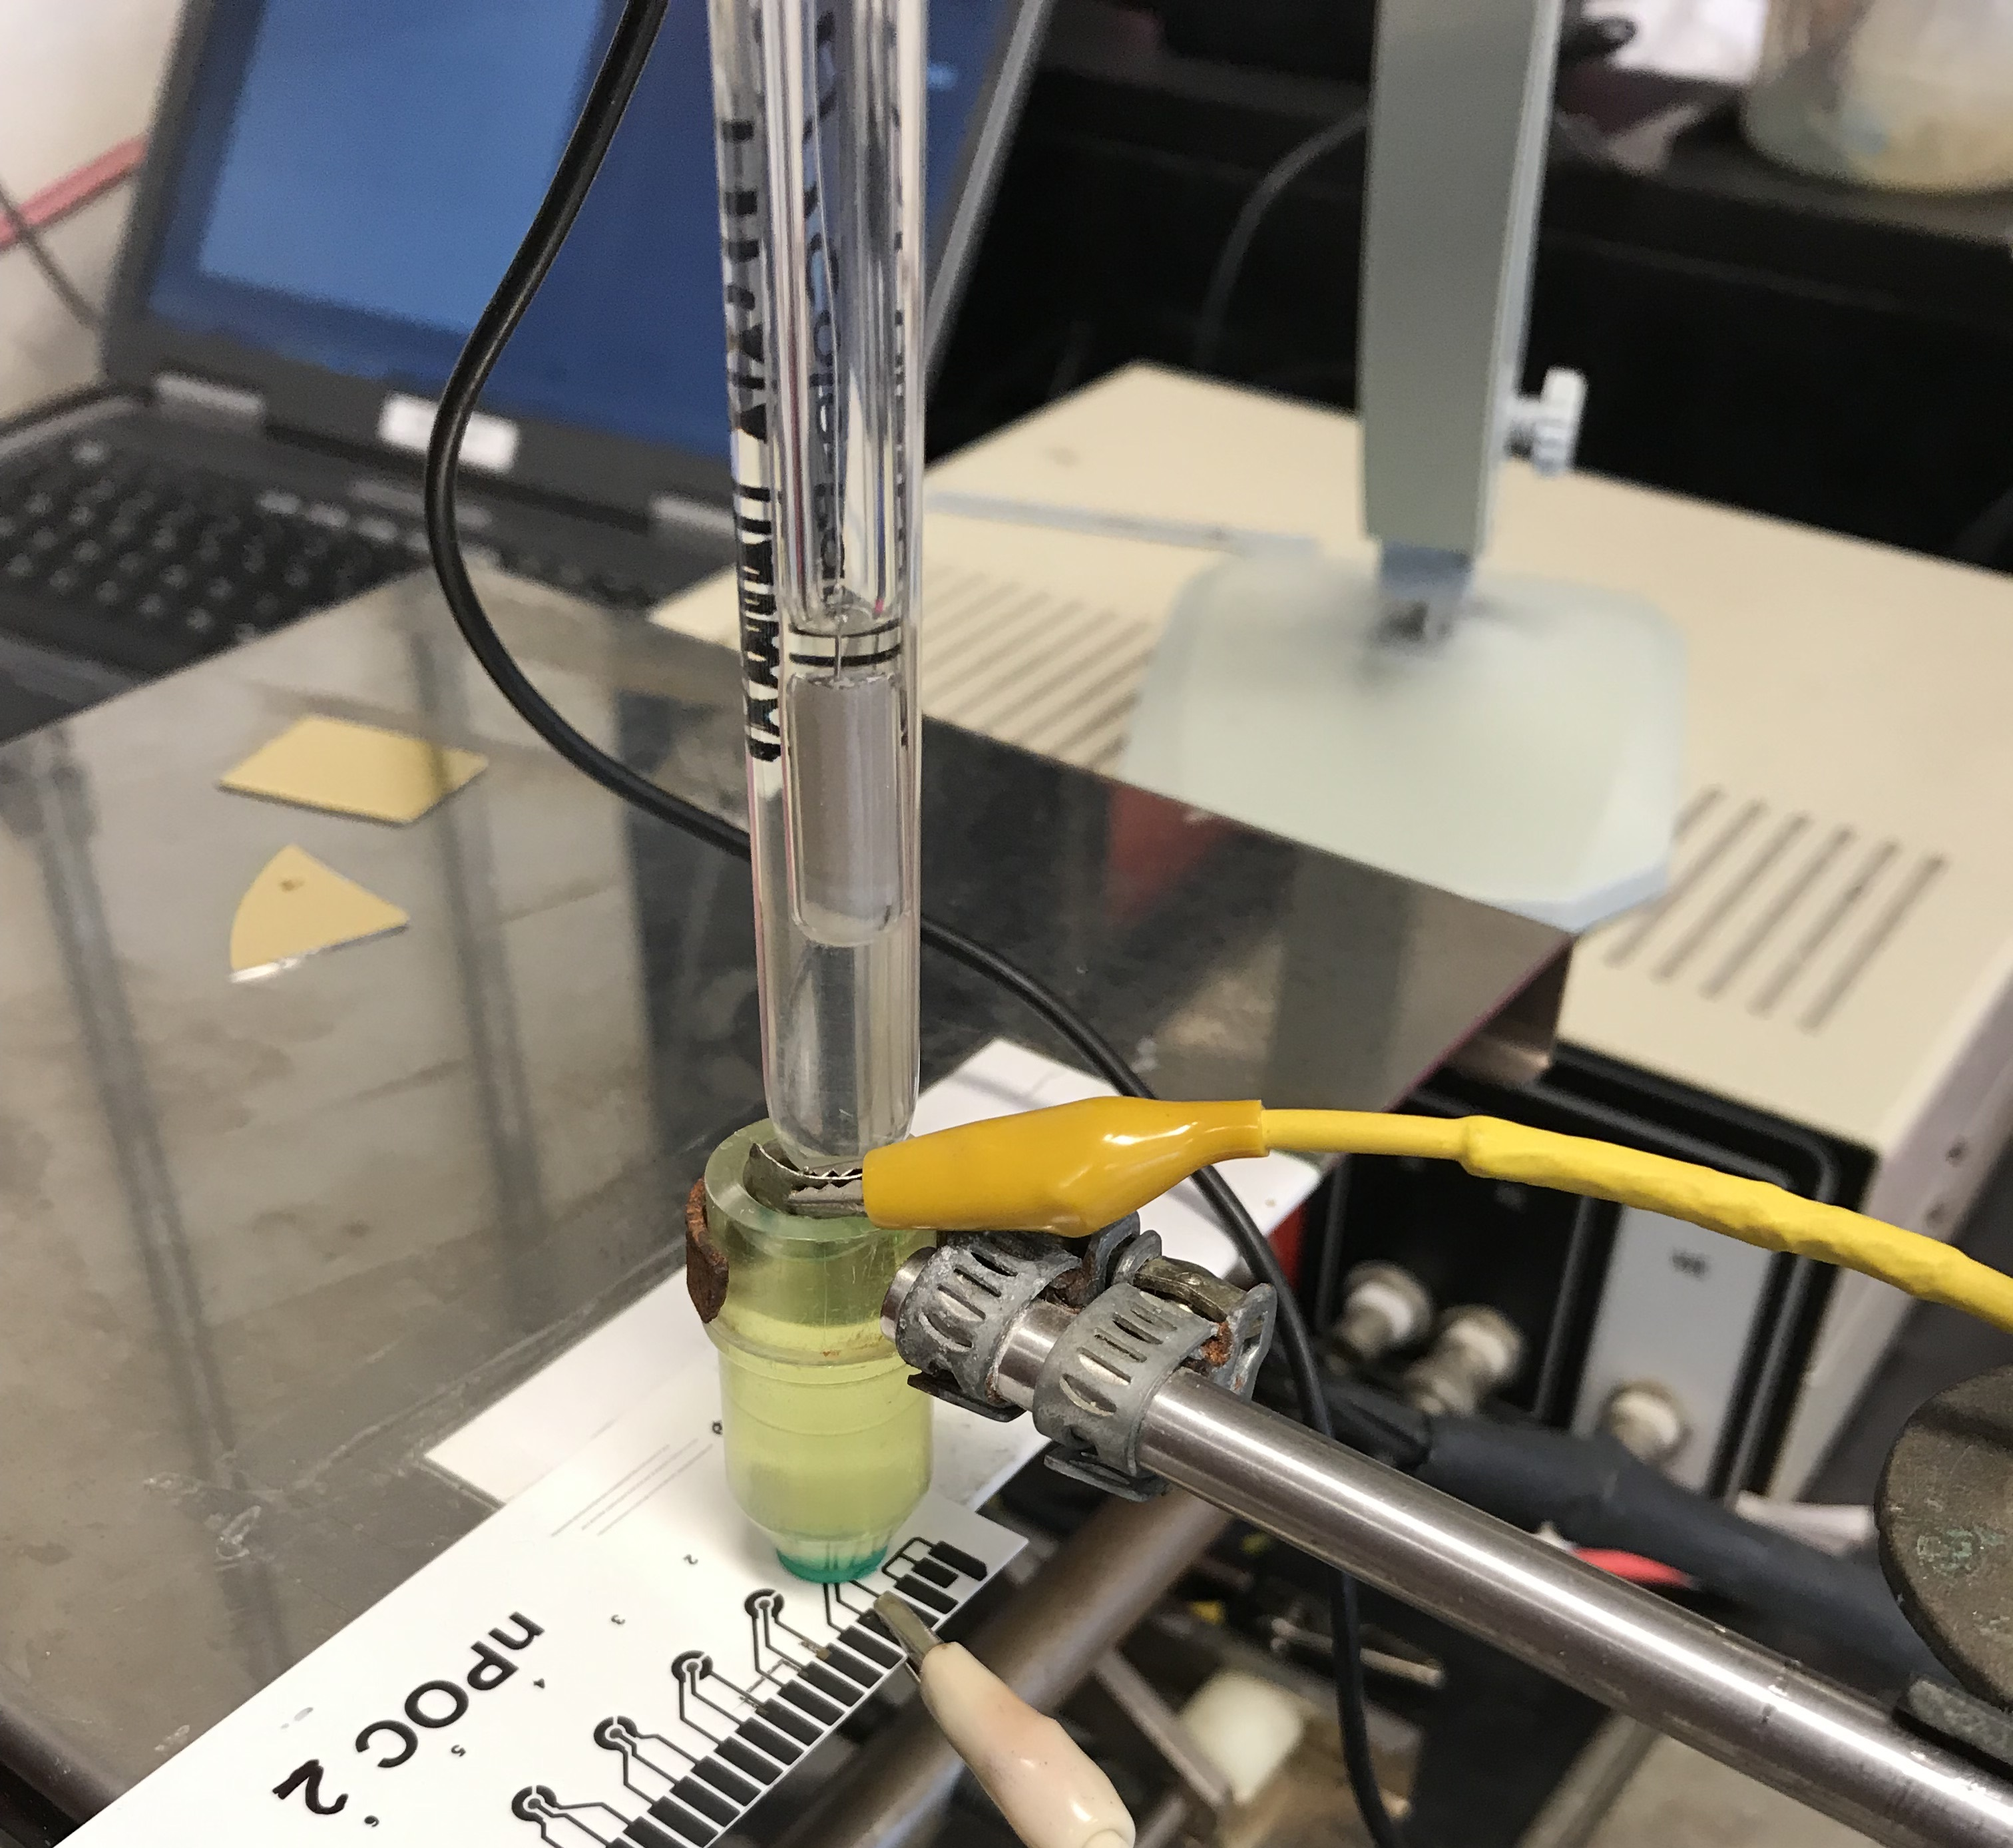
\includegraphics[width=0.5\textwidth]{Figures/Figura_prueba_electroquimica}
  \caption{Experimental setup for electrochemical measurements.}
  \label{fig:Figura_prueba_electroquimica}
\end{figure}

Special care must be taken so that the seal does not obstruct part of the working electrode, otherwise it will not be completely covered by the probe solution (Figure ~\ref{fig:Figura_electrodo_sonda}). In addition, it must be verified that when filling the cuvette no bubbles are formed, since the working electrode would not be completely covered either.

\begin{figure}[H]
  \centering
    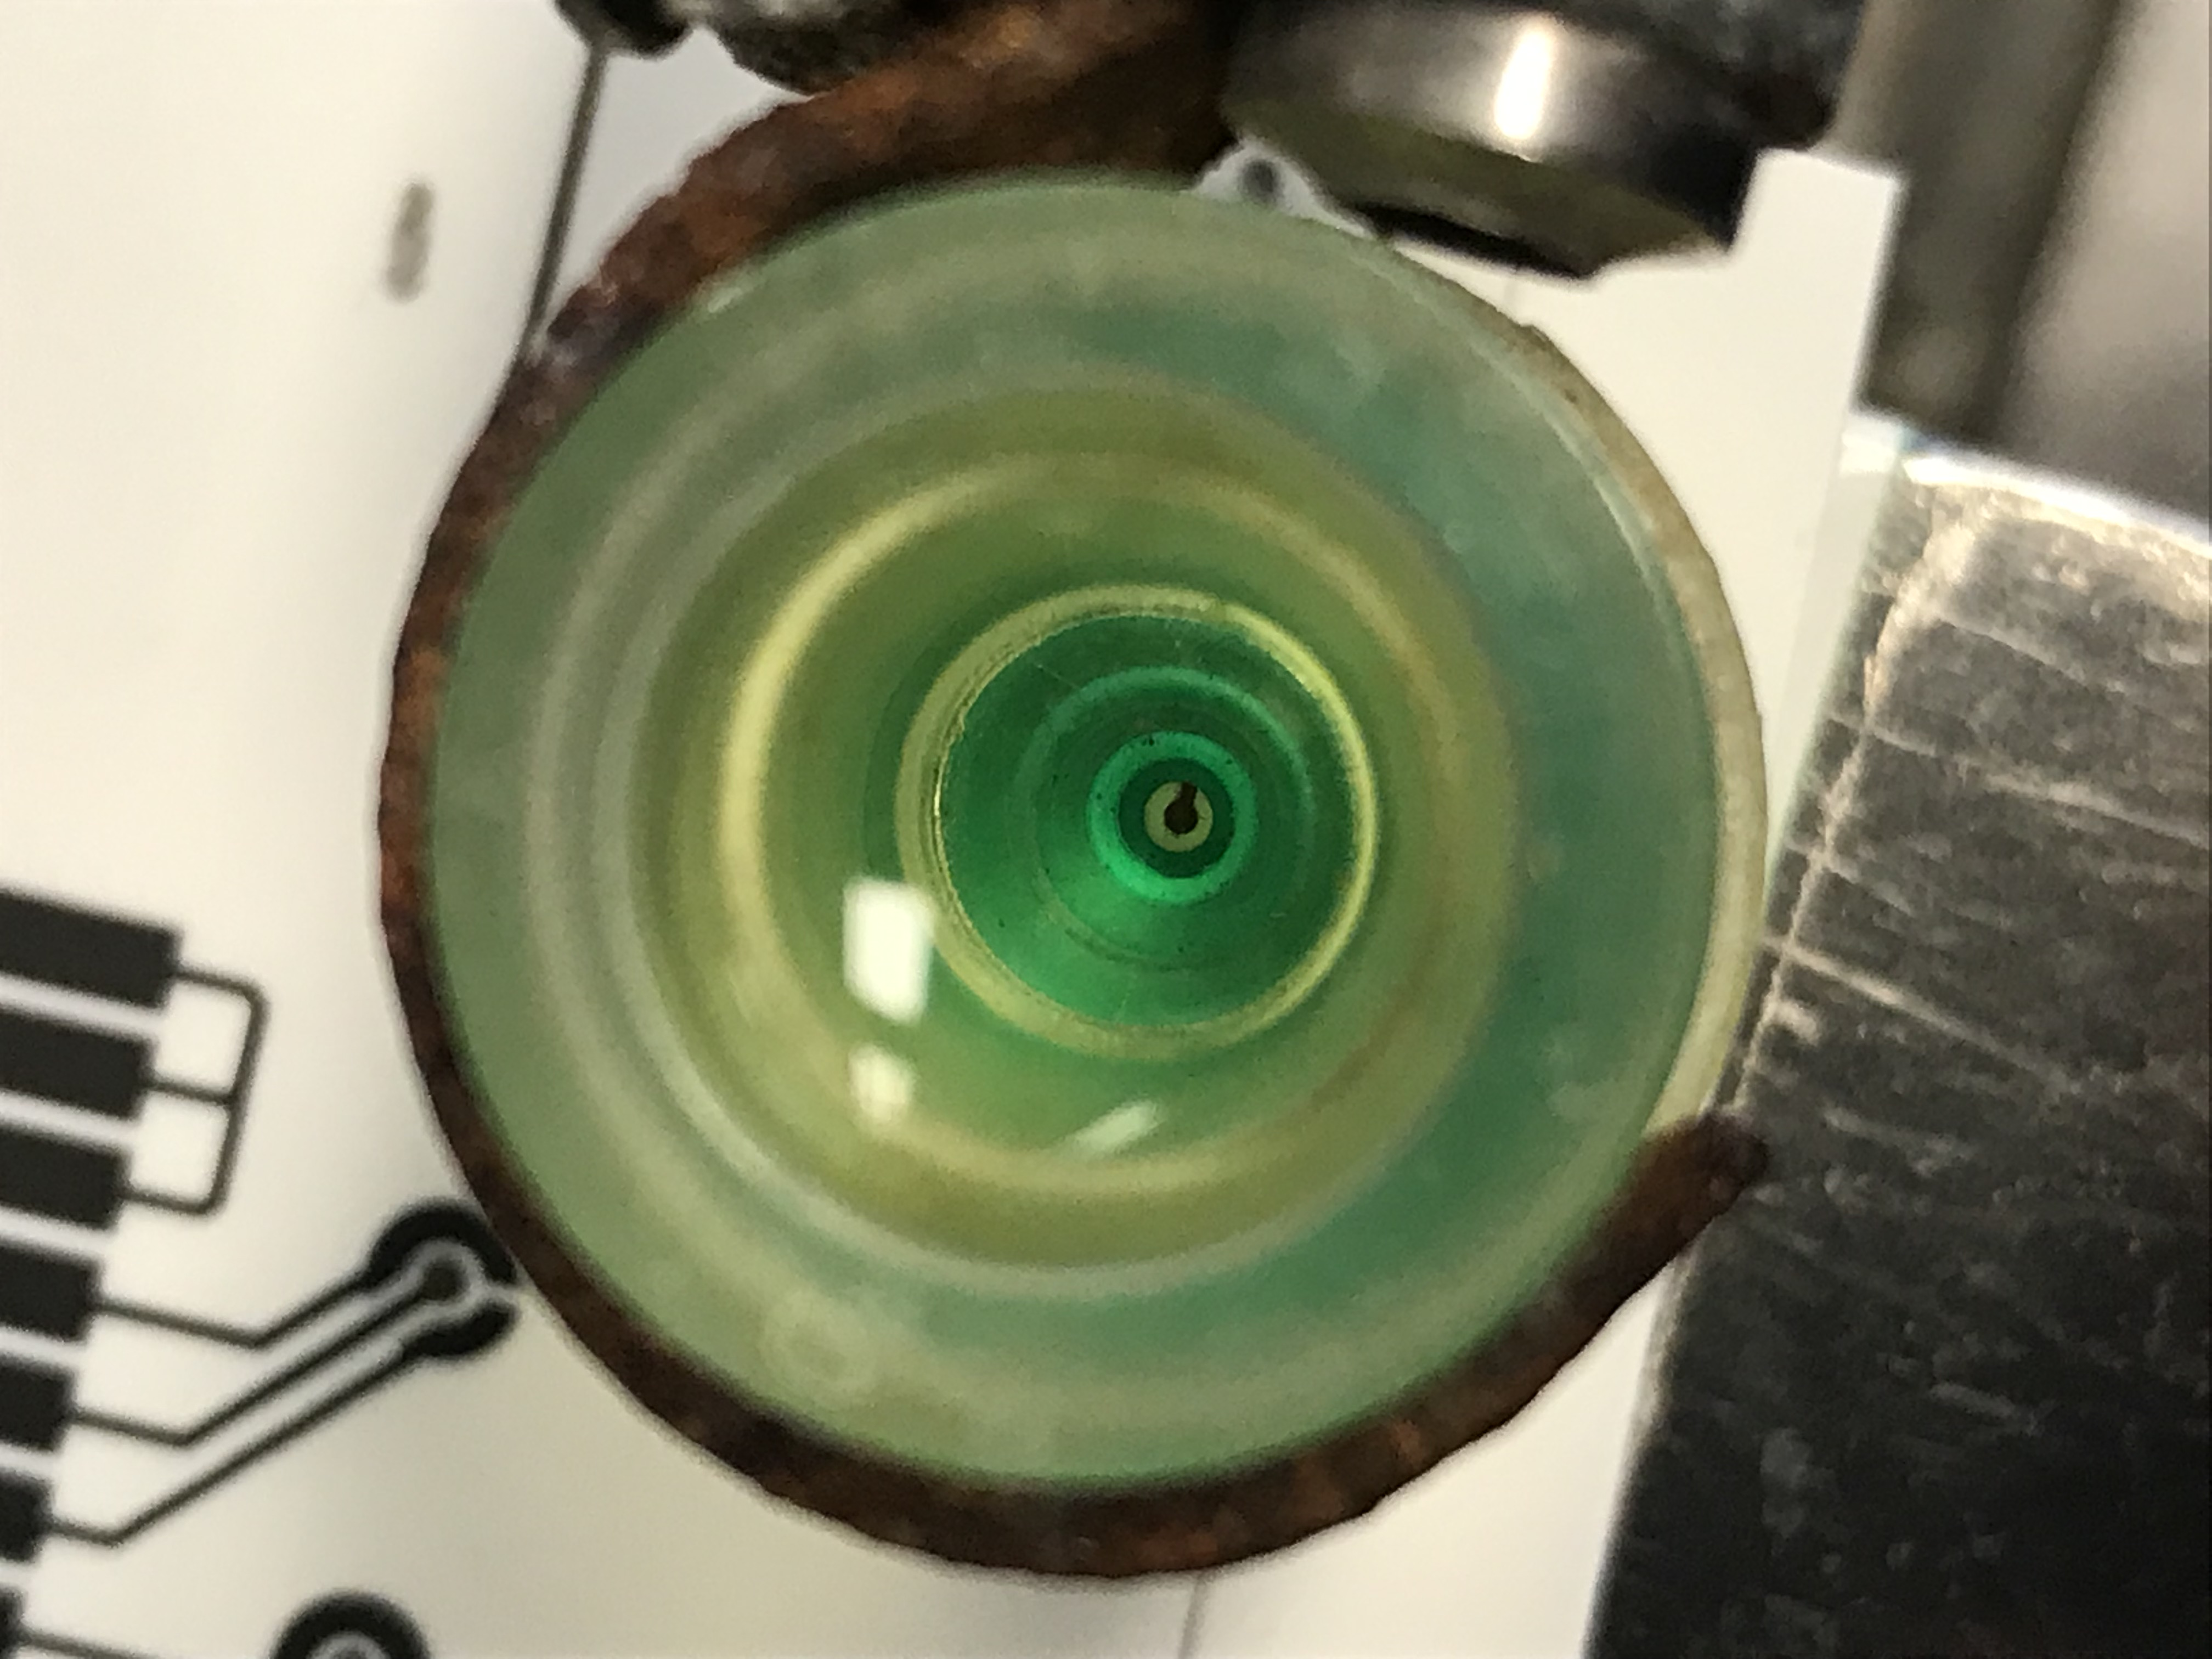
\includegraphics[width=0.5\textwidth]{Figures/Figura_electrodo_sonda}
  \caption{View of the Electrode in the acrylic cell.}
  \label{fig:Figura_electrodo_sonda}
\end{figure}

Measurements were taken with a \textit{Teq4} potentiostat. The excitation signal is a linear potential sweep with a triangular waveform of minimum potential E1 (-200 mV) and a maximum potential E2 (500 mV), with a sweep speed of 50 mV·s\textsuperscript{-1}. Using the potentiostat software, voltages and currents data were taken and exported in \textit{comma separated values} (CSV) format to be further processed in open source software \textit{GNUplot}. In addition, the graphics made by the potentiostat software were saved in PNG format as reference (Figure ~\ref{fig:Figura_software_potenciostato}).

\begin{figure}[H]
  \centering
    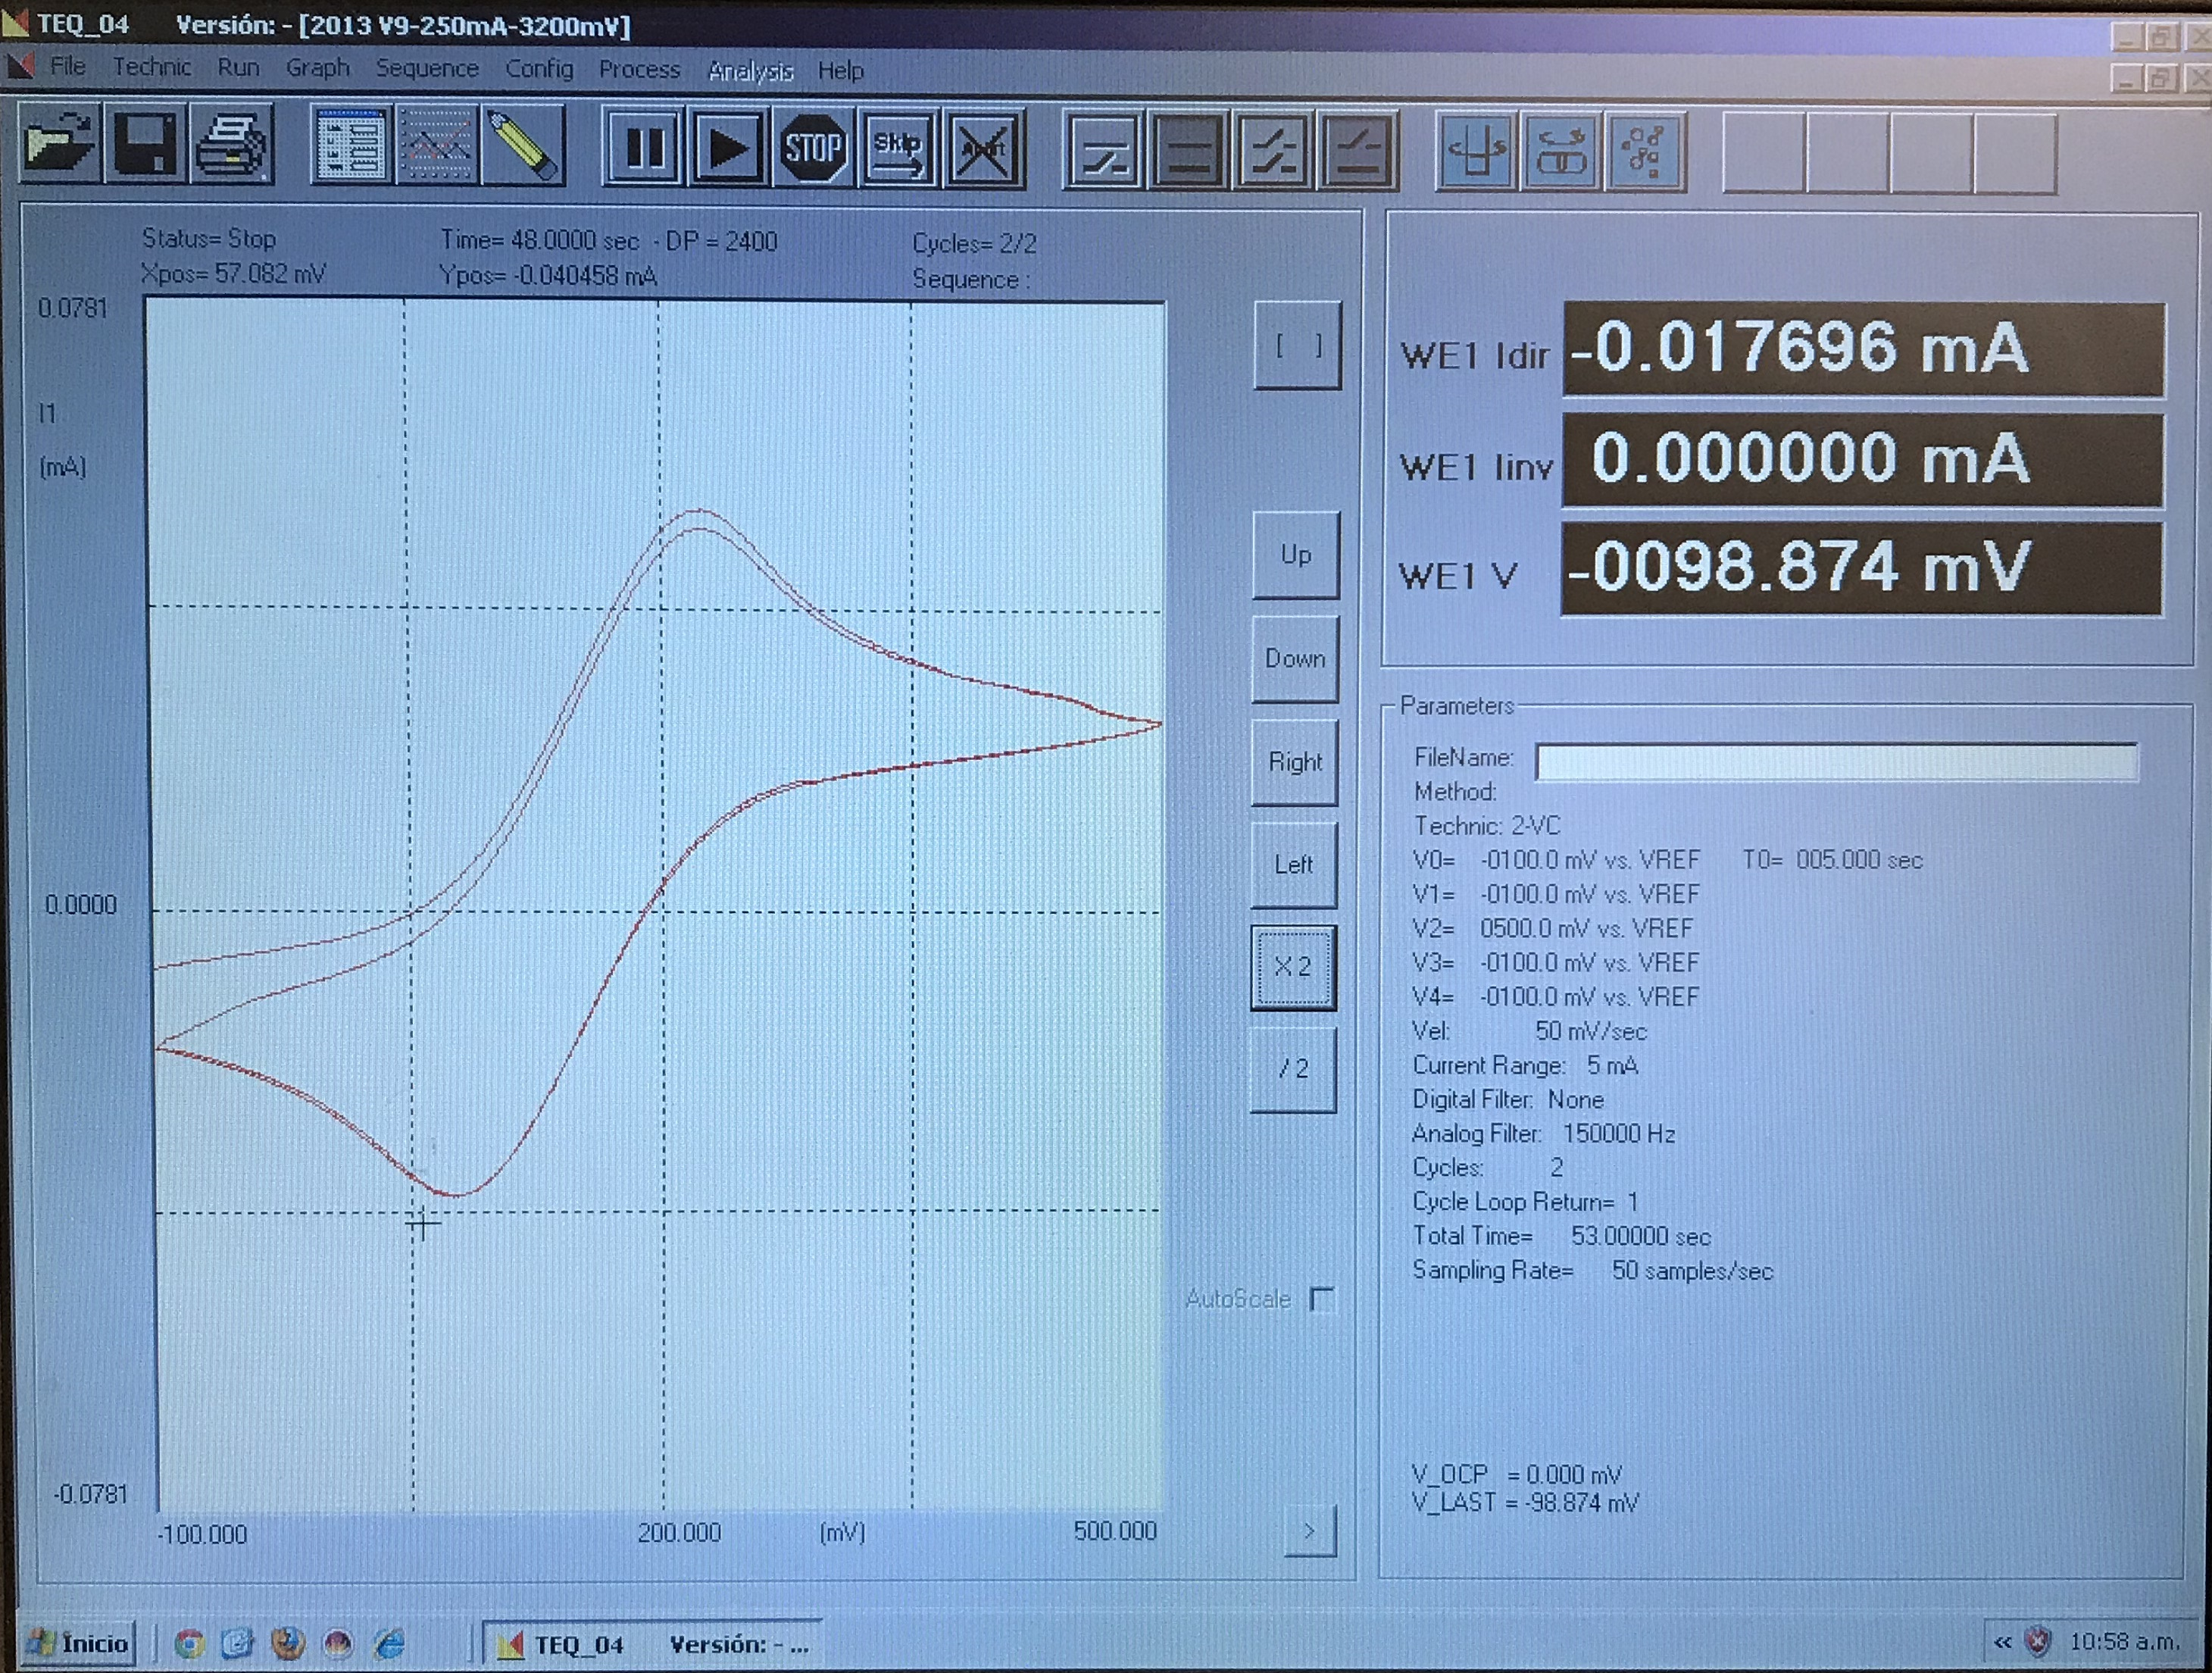
\includegraphics[width=0.5\textwidth]{Figures/Figura_software_potenciostato}
  \caption{\textit{Teq4} potentiostat software with measurement graph.}
  \label{fig:Figura_software_potenciostato}
\end{figure}

Once the experiments were carried out on all the samples, the data was processed to know the results and conclusions of the project.

\section{Photo-definable dielectric ink}
\label{sec:tinta_dielec}
This section will set out a project to continue, as a next step to the printing of gold nanoparticles on the working electrodes. Using the photo-definable dielectric ink, micro cuvettes will be made around the \emph{WE}. To generate these 3D structures by \textit{Inkjet} printing, several layers must be printed with their respective cures, forming a cylinder centered on each of the eight \emph{WE}. In this way, it is sought to form a container for each electrochemical cell, where the samples to be analyzed will be deposited. The main advantage for which this project is proposed is to use the \textit{Inkjet} printer for the complete manufacture of the biosensor, without the need to use other processes.

\subsection{Design}
Taking the dimensions of the working electrodes, 3 rings of different sizes were designed as a first approximation. These figures, printed in several layers, will form the microcuvette that will keep the sample contained on the electrochemical cell. The dimensions of the designs were 1050, 1100 and 1150 $\mu$m internal radius and 1350, 1300 and 1250 $\mu$m external radius, respectively. (Figure ~\ref{fig:Figura_anillos_SU8}).

\begin{figure}[H]
  \centering
    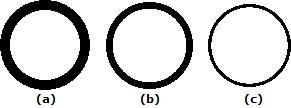
\includegraphics[width=0.5\textwidth]{Figures/Figura_anillos_SU8}
  \caption{(a) Ring from 1050 to 1350 $\mu$m. (b) Ring from 1100 to 1300 $\mu$m. (c) Ring from 1150 to 1250 $\mu$m.}
  \label{fig:Figura_anillos_SU8}
\end{figure}

In this way rings of 100, 200 and 300 $\mu$m thick are obtained, with which the optimal values for the printing of several successive layers will be determined, forming the microcuvette.

\subsection{Ink cartridge preparation}
For the formulation of the ink, a resin called \textit{SU-8 2007} was used as the solute and Cyclohexanone as the solvent (Figure ~\ref{fig:Figura_SU8_Ciclohexanona}). To obtain the proper viscosity to form and eject the ink droplets, the necessary proportion of each compound was calculated. It was determined that 2 ml of Cyclohexanone is necessary for every 3 ml of \textit{SU-8 2007}.

\begin{figure}[H]
  \centering
    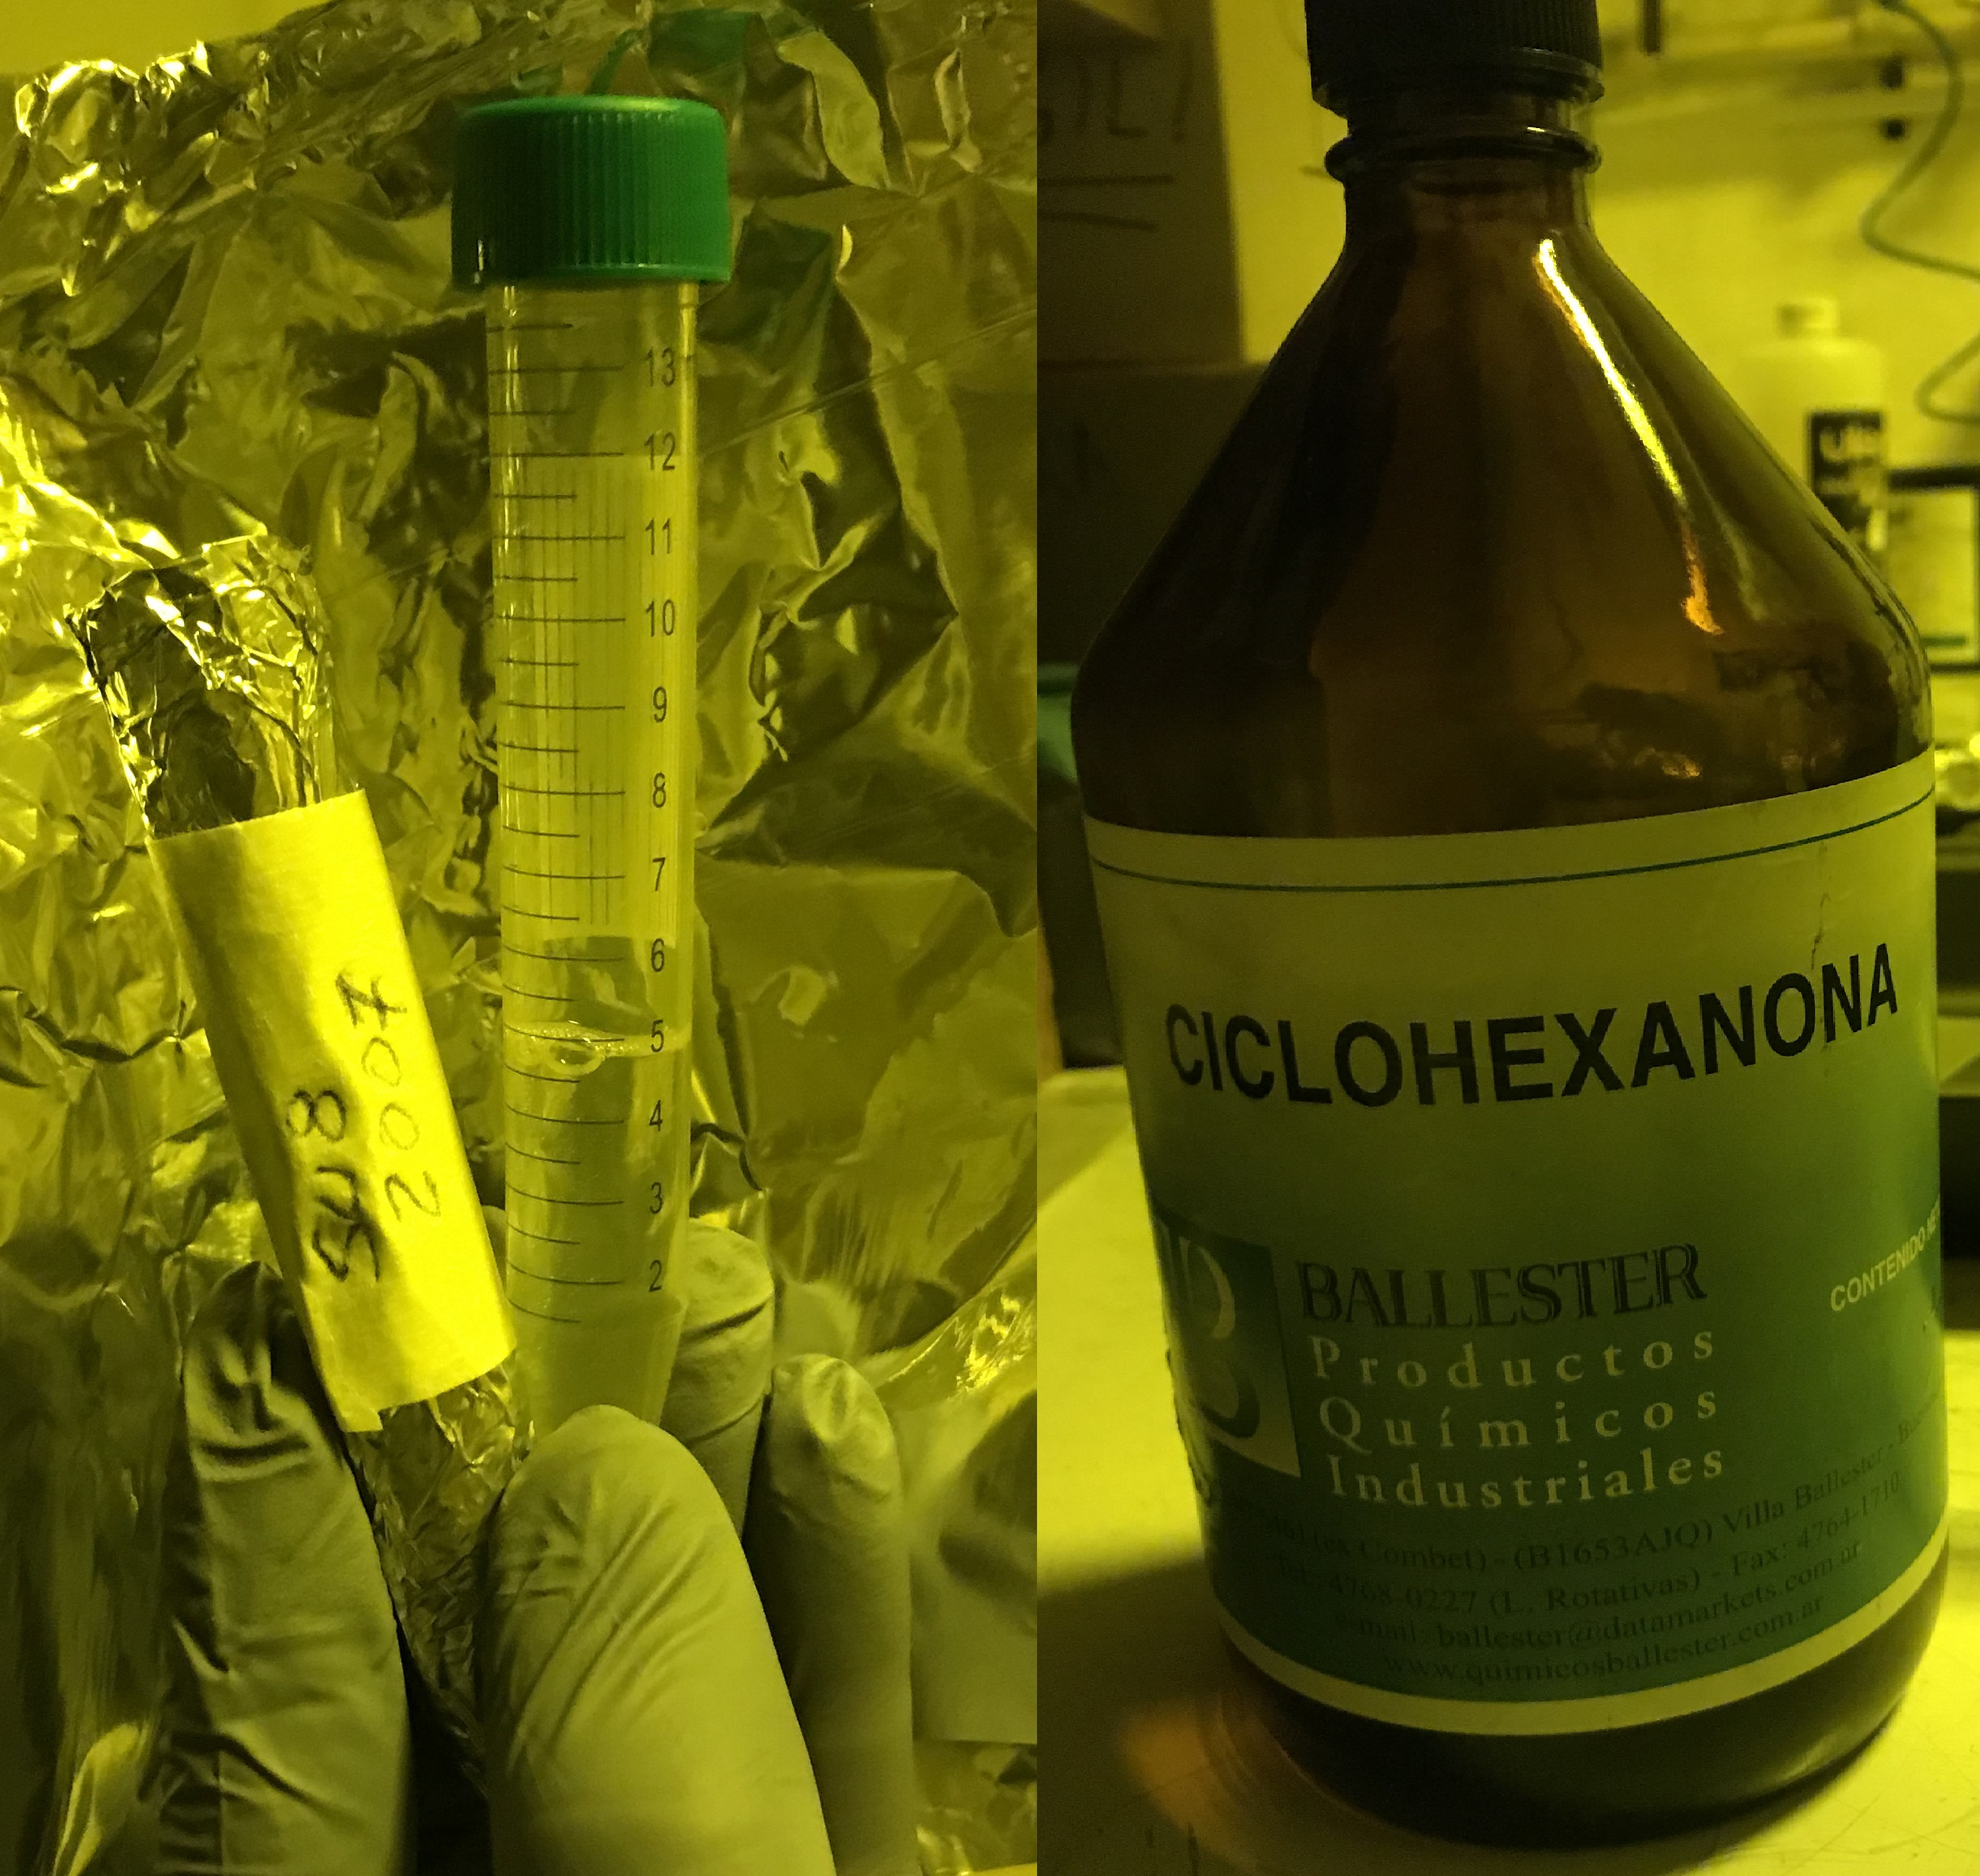
\includegraphics[width=0.5\textwidth]{Figures/Figura_SU8_Ciclohexanona}
  \caption{Solute and solvent to formulate the photo-definable dielectric ink.}
  \label{fig:Figura_SU8_Ciclohexanona}
\end{figure}

Since said solute is photosensitive, the preparation had to be done in a dark room with UV filters. The cartridge reservoir had to be protected from UV rays because the printer is not in a dark room with the appropriate filters, which would dry the ink inside the reservoir. For this, aluminum foil was used, forming a cover, without blocking the head and its connections with the reel (Figure ~\ref{fig:Figura_cartucho_SU8}).

\begin{figure}[H]
  \centering
    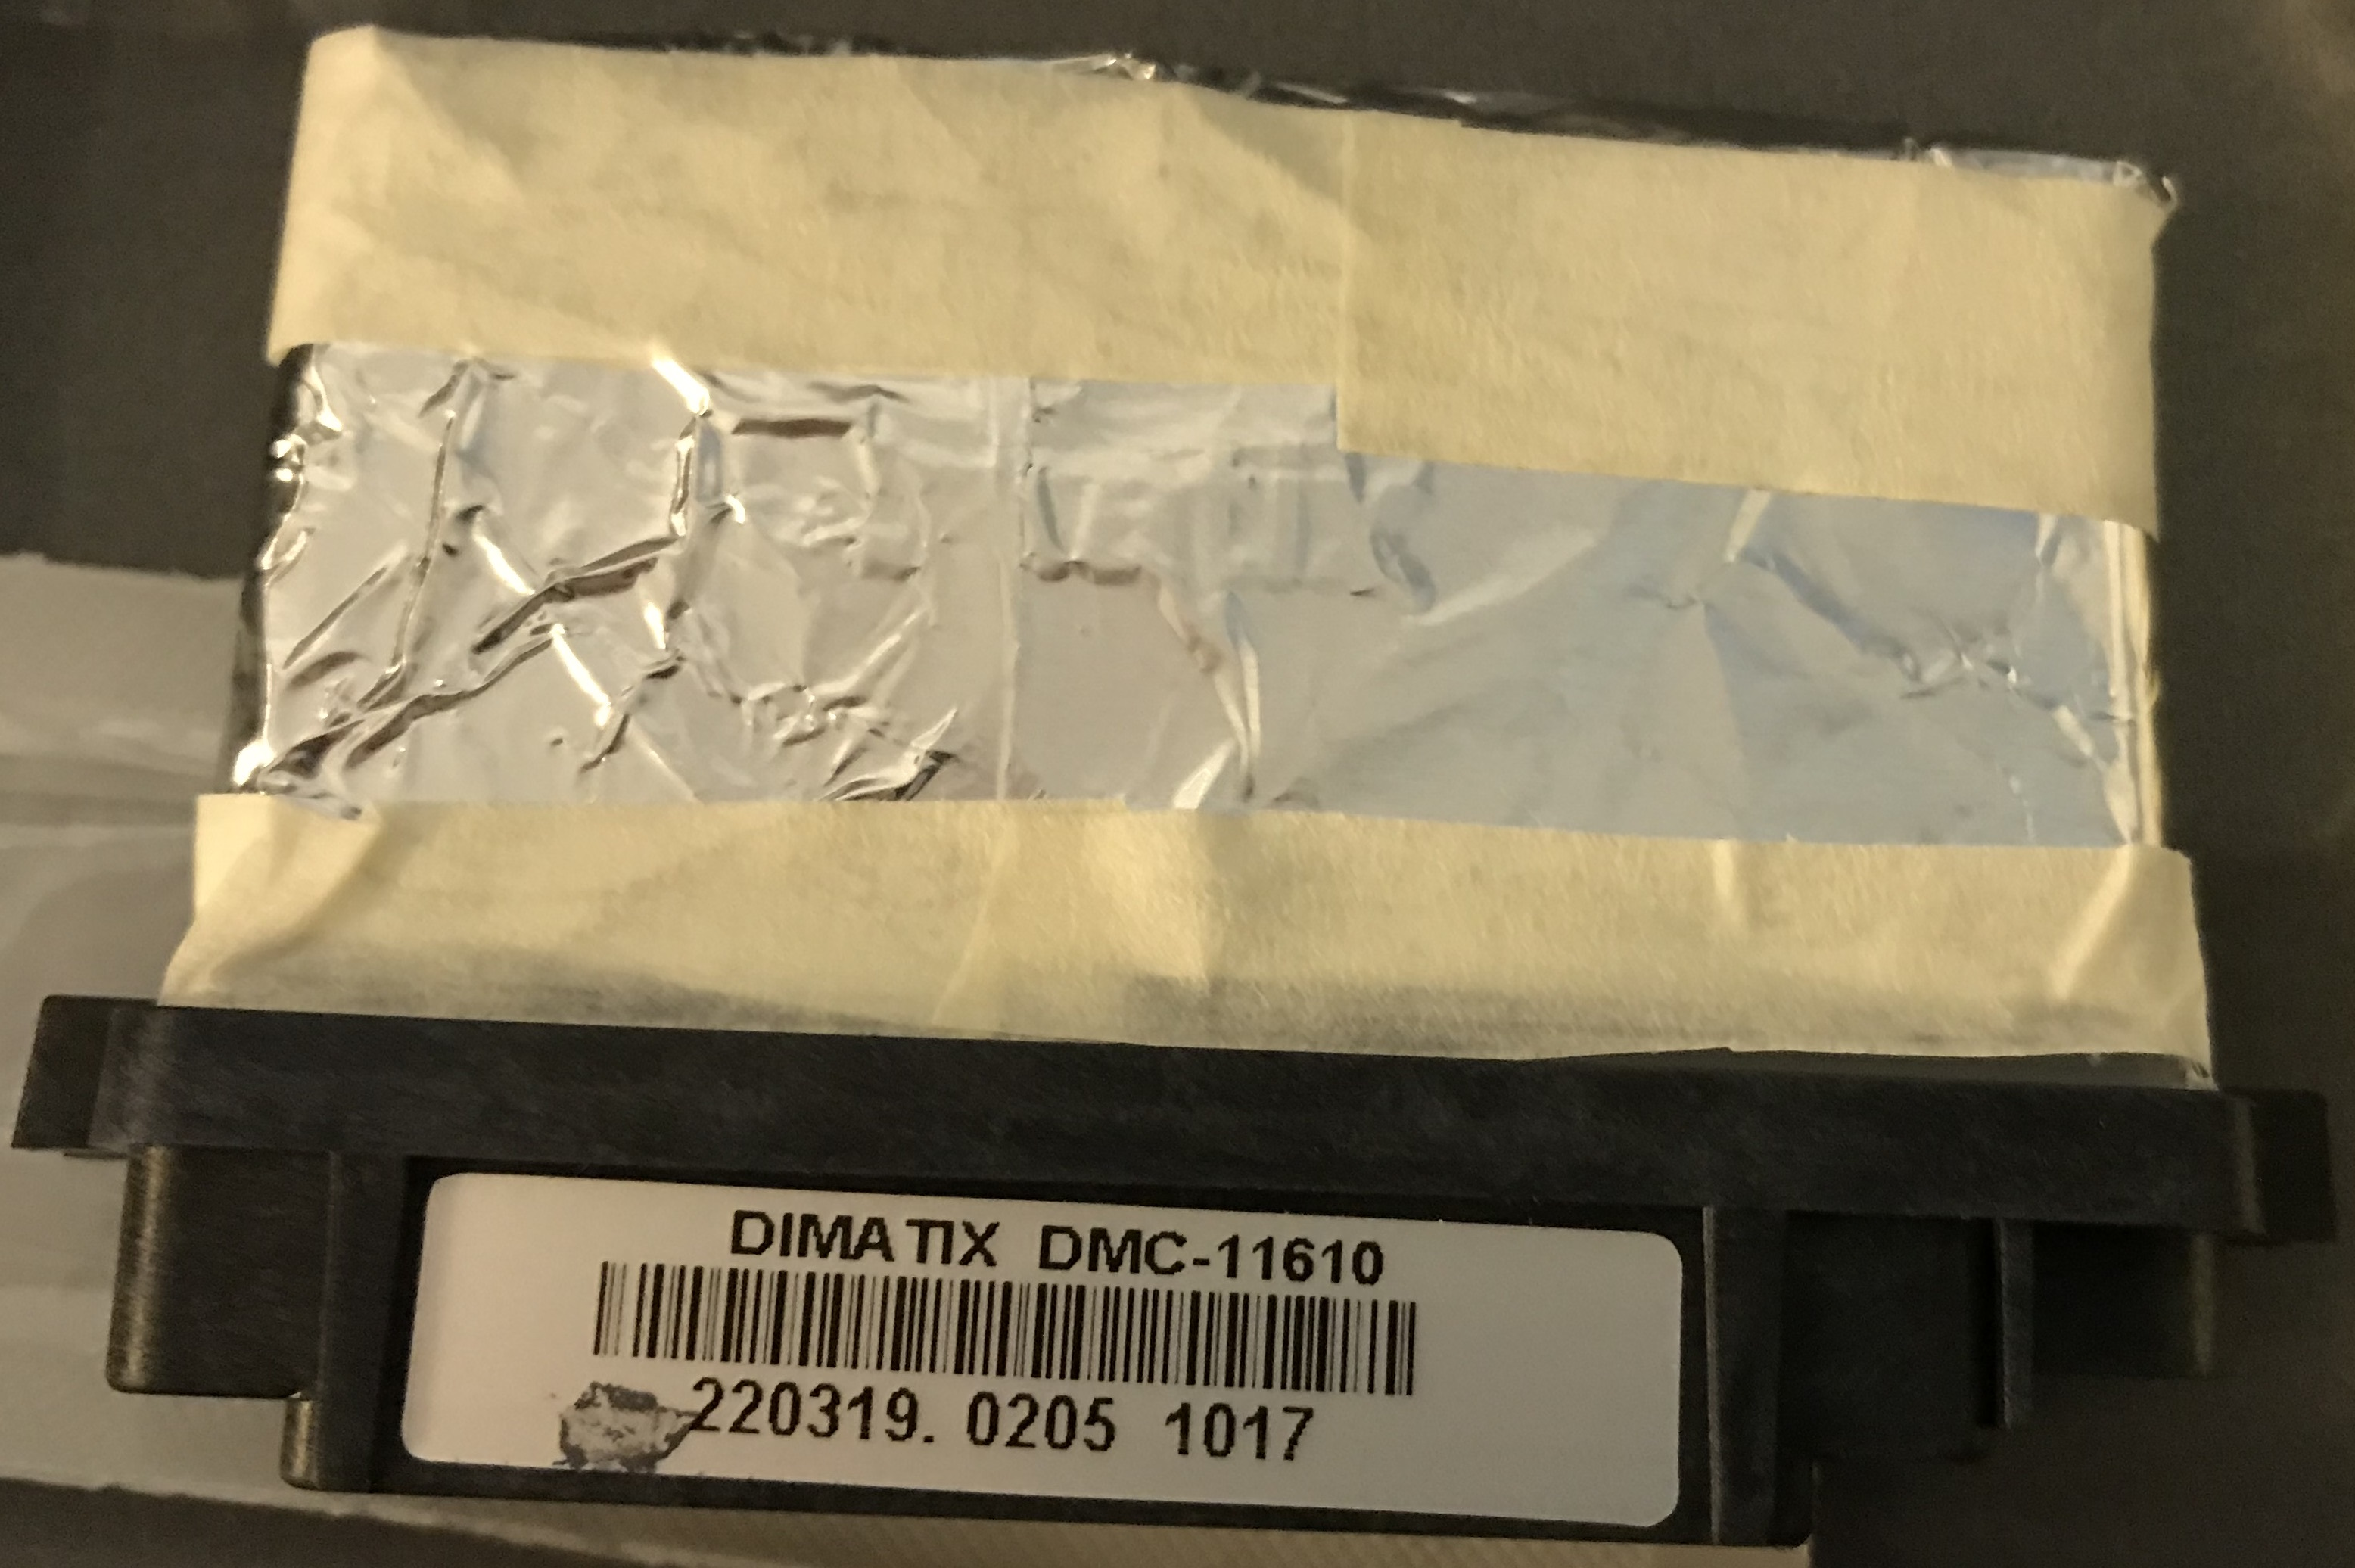
\includegraphics[width=0.5\textwidth]{Figures/Figura_cartucho_SU8}
  \caption{SU-8 ink cartridge protected from UV rays.}
  \label{fig:Figura_cartucho_SU8}
\end{figure}

\subsection{Printer setup and calibration}
When installing the ink cartridge in the printer, the parameters of the ink cartridge were configured using the information provided by the manufacturer \textit{Microchem} \cite{PriElexSU8}, and the first ink ejection tests were carried out on the \textit{Drop Watcher} (Figure ~\ref{fig:Figura_Drop_Watcher_SU8}).

\begin{figure}[H]
  \centering
    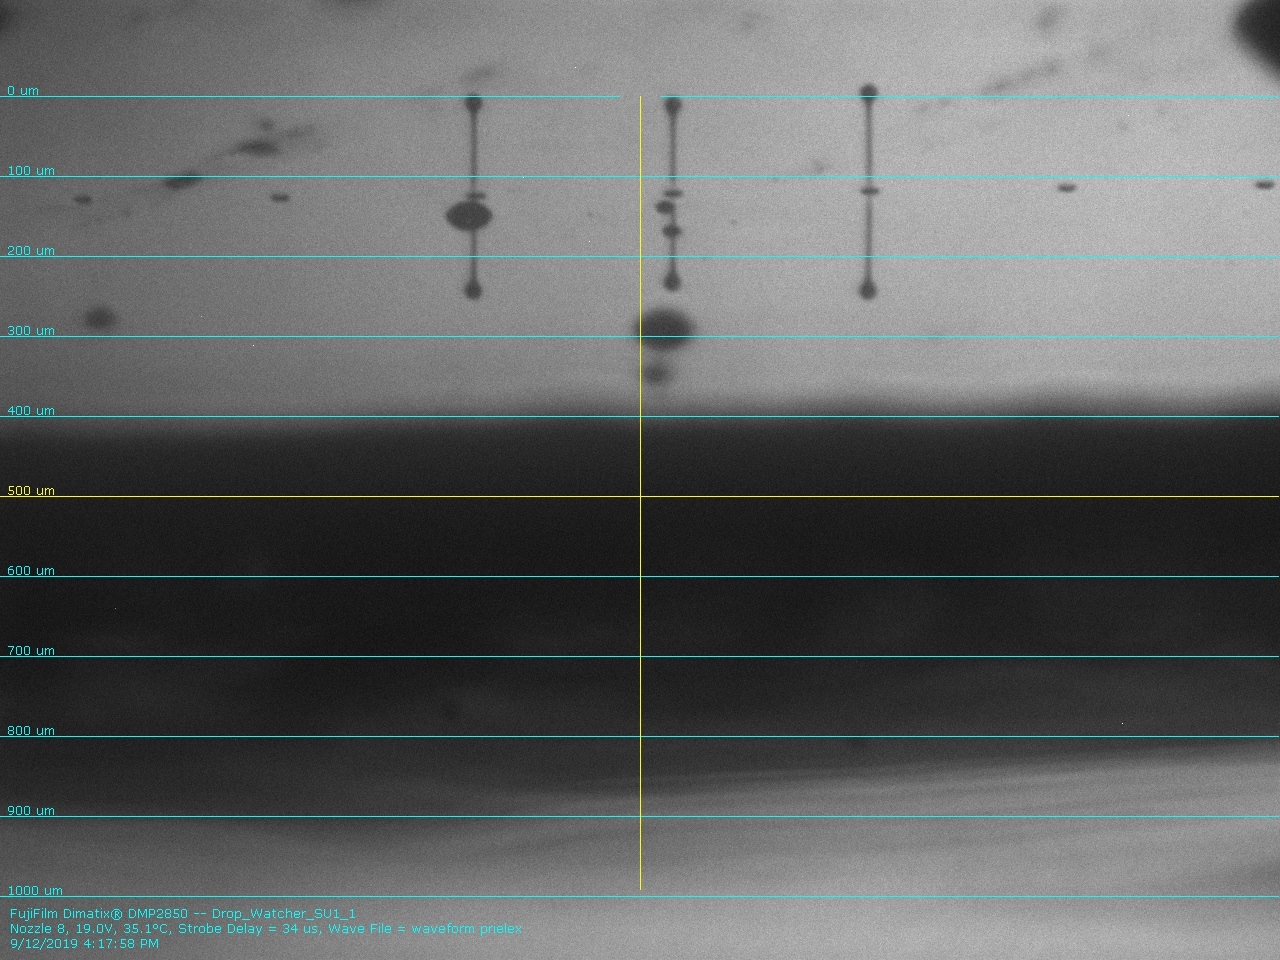
\includegraphics[width=0.5\textwidth]{Figures/Figura_Drop_Watcher_SU8}
  \caption{SU-8 drops seen from the \textit{Drop Watcher} camera.}
  \label{fig:Figura_Drop_Watcher_SU8}
\end{figure}

Several purge cycles were necessary to obtain droplet ejection. The voltages of the nozzles were calibrated to have the same flight time between the 3 ejectors to be used.

\subsection{Prints}
The $``$\textit{Line Pattern}$"$ file was printed in order to define the spacing between drops necessary to obtain a continuous line with \textit{SU-8} ink on \textit{Valox} substrate. The optimal \textit{Drop Spacing}was defined to be 15 $\mu$m (Figure ~\ref{fig:Figura_LinePattern_SU8}).

\begin{figure}[H]
  \centering
    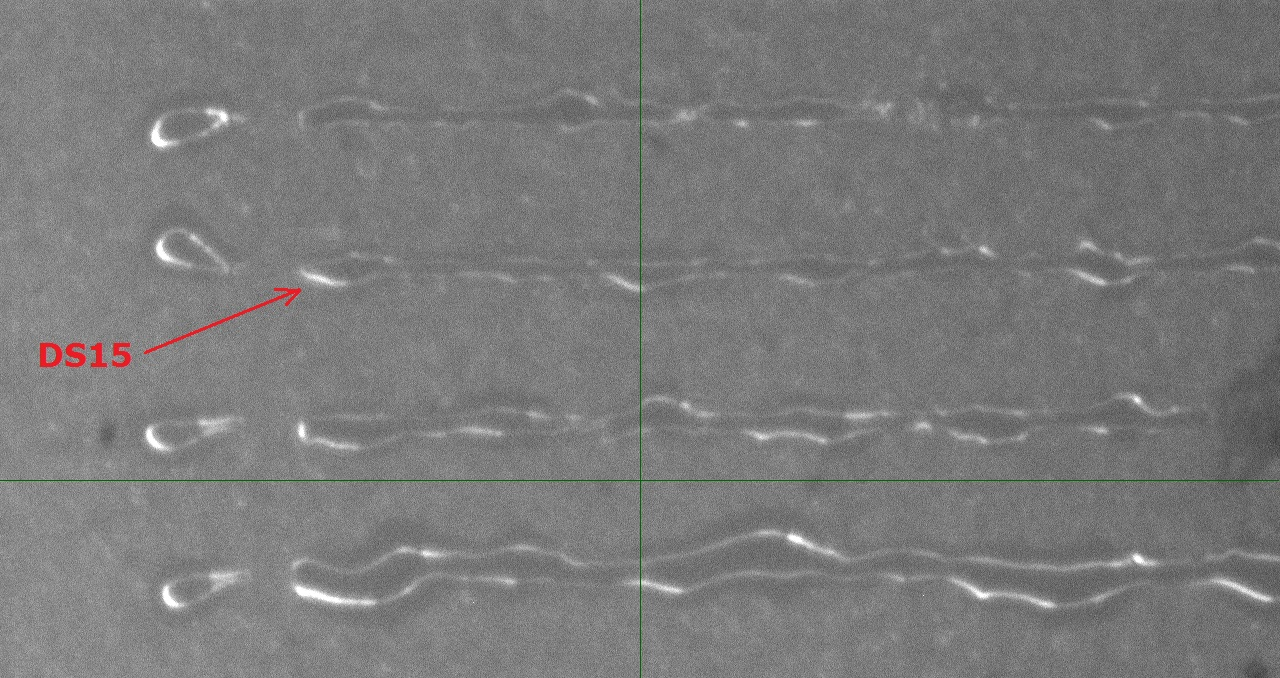
\includegraphics[width=0.5\textwidth]{Figures/Figura_LinePattern_SU8}
  \caption{Enlarged image of $``$\textit{Line Pattern}$"$ print.}
  \label{fig:Figura_LinePattern_SU8}
\end{figure}

For this \emph{DS}, the files to be printed must have a resolution of 1693.33 dpi as previously seen in Chapter 3, \hyperref[sec:calib_impresora]{section 3.2}.

Once the imported files were configured using the \textit{DMP} software, the first ring of radii 1050 $\mu$m inside and 1350 $\mu$m outside was printed (Figure ~\ref{fig:Figura_Anillo105a135_SU8}).

\begin{figure}[H]
  \centering
    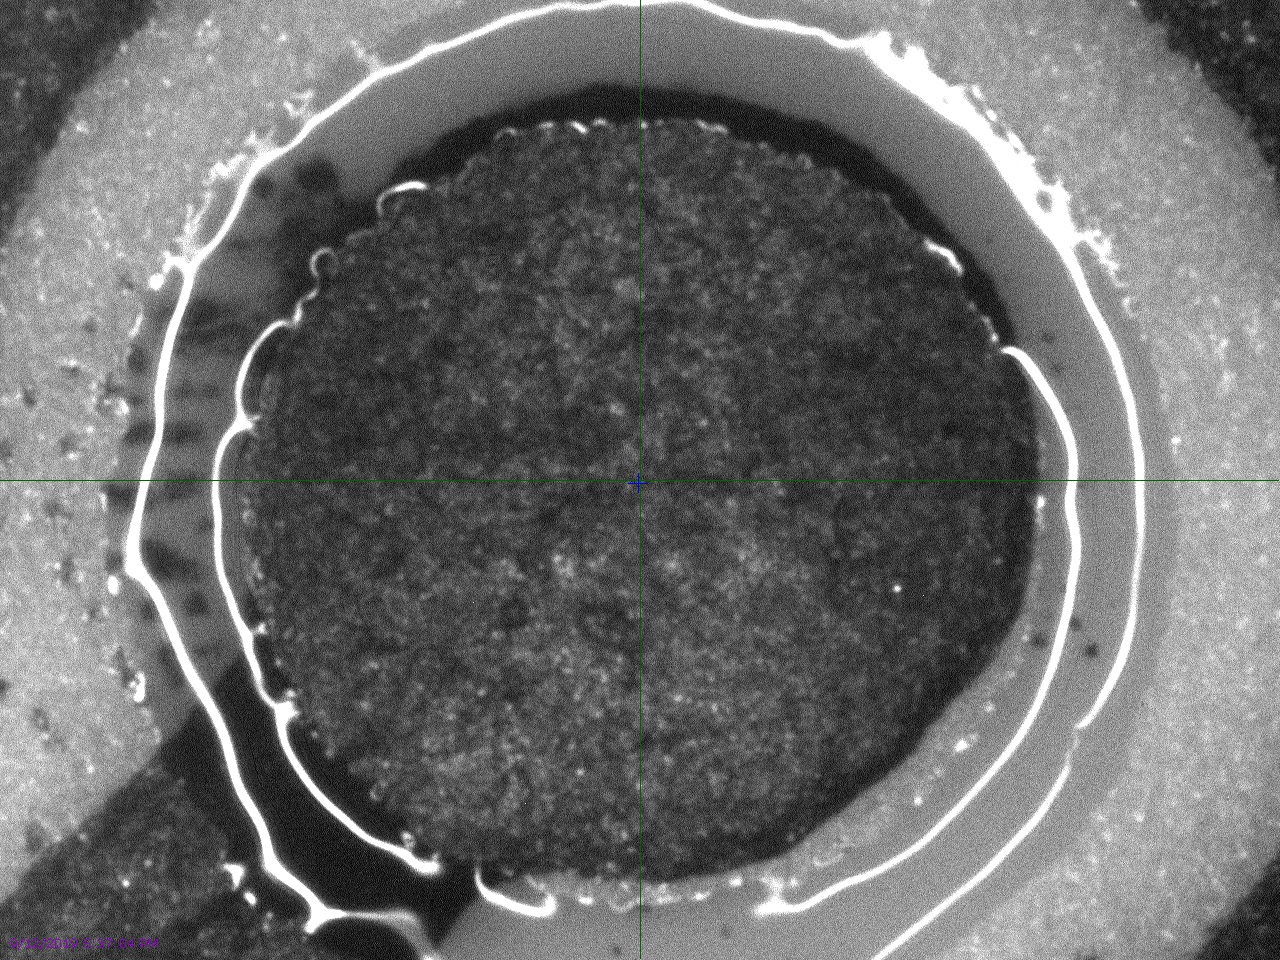
\includegraphics[width=0.5\textwidth]{Figures/Figura_Anillo105a135_SU8}
  \caption{Printing ring of radii 1050 $\mu$m inside and 1350 $\mu$m outside.}
  \label{fig:Figura_Anillo105a135_SU8}
\end{figure}

Subsequently, a ring with 1100 $\mu$m of internal and 1300 $\mu$m of external radio was printed (Figure ~\ref{fig:Figura_Anillo110a130_SU8}).

\begin{figure}[H]
  \centering
    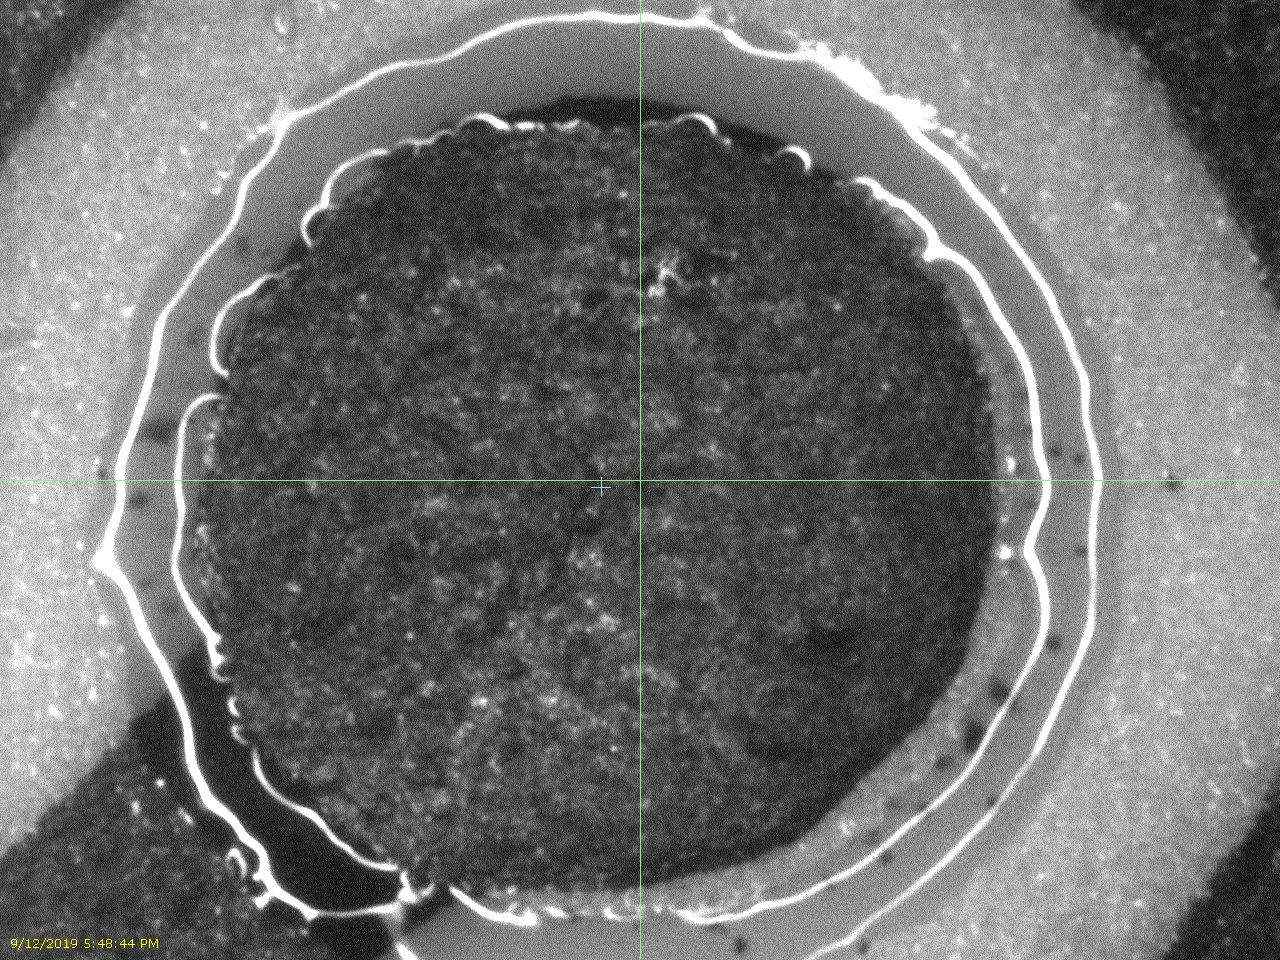
\includegraphics[width=0.5\textwidth]{Figures/Figura_Anillo110a130_SU8}
  \caption{Print of a ring with 1100 $\mu$m interior and 1300 $\mu$m exterior radio.}
  \label{fig:Figura_Anillo110a130_SU8}
\end{figure}

Finally, the 1150 $\mu$m interio and 1250 $\mu$m exterior radius ring was printed (Figure ~\ref{fig:Figura_Anillo115a125_SU8}).

\begin{figure}[H]
  \centering
    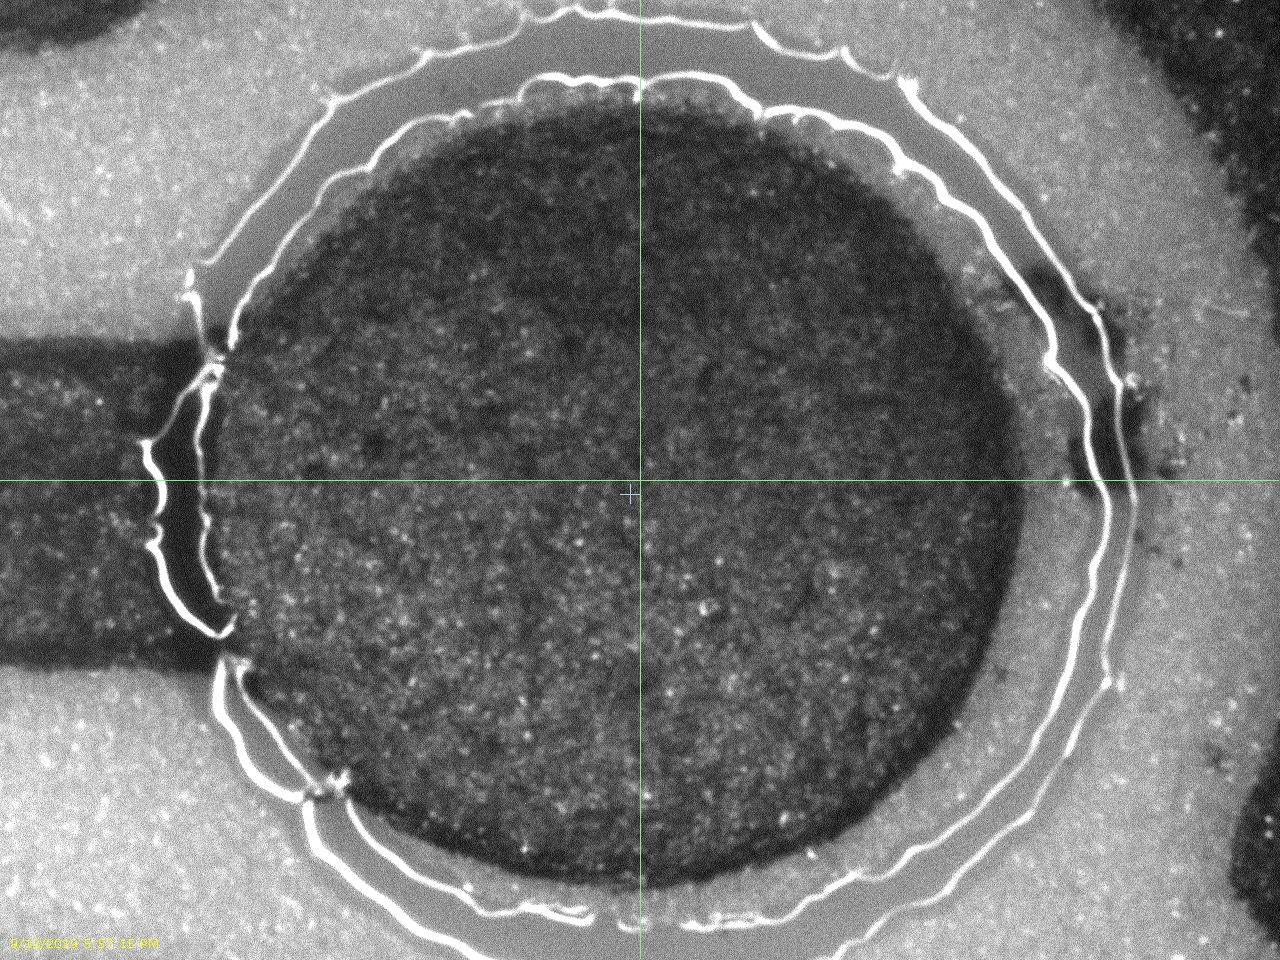
\includegraphics[width=0.5\textwidth]{Figures/Figura_Anillo115a125_SU8}
  \caption{Print of a ring with 1150 $\mu$m interior and 1250 $\mu$m exterior radio.}
  \label{fig:Figura_Anillo115a125_SU8}
\end{figure}

\subsection{Characterizations}
All new micro-cuvette electrochemical cell configurations, obtained by \textit{inkjet} printing with \textit{ad hoc} inks, will be characterized in future work.